% !TeX document-id = {6d0ae1f9-9569-4d0b-bd40-c08220393731}
% !TEX TS-program = XeLaTeX
% Command for running this example (needs latexmkrc file):
%    latexmk -bibtex -pdf main.tex

%	نمونه پایان‌نامه آماده شده با استفاده از کلاس tehran-thesis، نگارش 1
%	سینا ممکن، دانشگاه تهران 
%	https://github.com/sinamomken/tehran-thesis
%	گروه پارسی‌لاتک
%	http://www.parsilatex.com
%	این نسخه، بر اساس نسخه‌ 0.1 از کلاس IUST-Thesis آقای محمود امین‌طوسی آماده شده است.
%        http://profsite.sttu.ac.ir/mamintoosi

%----------------------------------------------------------------------------------------------
% اگر قصد نوشتن پروژه کارشناسی را دارید، در خط زیر به جای msc، کلمه bsc و اگر قصد نوشتن رساله دکترا را دارید، کلمه phd را قرار دهید. کلیه تنظیمات لازم، به طور خودکار، اعمال می‌شود.

% اگر مایلید پایان‌نامه شما دورو باشد به جای oneside در خط زیر از twoside استفاده کنید.

% برای حاشیه‌نویسی و کم کردن صفحات ابتدایی، گزینه draft را وارد و برای نسخه نهایی آن را حذف کنید.

% برای استفاده از قلم‌های سری IR Series گزینه irfonts را وارد و برای استفاده از قلم‌های X Series 2 آن را حذف کنید.

\documentclass[
twoside
% ,openany
,msc
,irfonts
% ,draft
]{./tex/tehran-thesis}

% فایل commands.tex را مطالعه کنید؛ چون دستورات مربوط به فراخوانی بسته‌ها، فونت و دستورات خاص در این فایل قرار دارد.

% در این فایل، دستورها و تنظیمات مورد نیاز، آورده شده است.
%-------------------------------------------------------------------------------------------------------------------
% دستوراتی که پوشه پیش‌فرض زیرفایل‌های tex را مشخص می‌کند.
%\makeatletter
%\def\input@path{{./tex/}}
%\makeatother
% در ورژن جدید زی‌پرشین برای تایپ متن‌های ریاضی، این سه بسته، حتماً باید فراخوانی شود
\usepackage{amsthm,amssymb,amsmath}
\DeclareMathOperator*{\argmin}{arg\,min}
% بسته‌ای برای تنطیم حاشیه‌های بالا، پایین، چپ و راست صفحه
\usepackage[a4paper, top=40mm, bottom=40mm, outer=25mm, inner=35mm]{geometry}
% بسته‌‌ای برای ظاهر شدن شکل‌ها و تعیین آدرس تصاویر
\usepackage[final]{graphicx}
\graphicspath{{./img/}}
% بسته‌های مورد نیاز برای نوشتن کدها، رنگ‌آمیزی آنها و تعیین پوشهٔ کدها
\usepackage[final]{listings}
\usepackage[usenames,dvipsnames,svgnames,table]{xcolor}
\lstset{inputpath=./code/}
% بسته‌ای برای رسم کادر
\usepackage{framed} 
% بسته‌‌ای برای چاپ شدن خودکار تعداد صفحات در صفحه «معرفی پایان‌نامه»
\usepackage{lastpage}
% بسته‌ٔ لازم برای: ۱. تغییر شماره‌گذاری صفحات پیوست. ۲. تصحیح باگ آدرس وب حاوی '%' در مراجع
\usepackage{etoolbox}

%%%%%%%%%%%%%%%%%%%%%%%%%%%%%%%%%%%%
%%% دستورات وابسته به استیل مراجع:
%% اگر از استیل‌های natbib (plainnat-fa، asa-fa، chicago-fa) استفاده می‌کنید، خط زیر را فعال و بعدی‌اش را غیرفعال کنید.
%\usepackage{natbib}
%\newcommand{\citelatin}[1]{\cite{#1}\LTRfootnote{\citeauthor*{#1}}}
%\newcommand{\citeplatin}[1]{\citep{#1}\LTRfootnote{\citeauthor*{#1}}}
%% اگر از سایر استیل‌ها استفاده می‌کنید، خط بالا را غیرفعال و خط‌های زیر را فعال کنید.
\let\citep\cite
\let\citelatin\cite
\let\citeplatin\cite
%%%%%%%%%%%%
% بررسی حالت پیش نویس
\usepackage{ifdraft}
\ifdraft
{%
	% بسته‌ٔ ایجاد لینک‌های رنگی با امکان جهش
	\usepackage[unicode=true,pagebackref=true,
colorlinks,linkcolor=blue,citecolor=blue,final]{hyperref}
	%\usepackage{todonotes}
	\usepackage[firstpage]{draftwatermark}
	\SetWatermarkText{\ \ \ پیش‌نویس}
	\SetWatermarkScale{1.2}
}
{ 
	\usepackage[pagebackref=false]{hyperref}
	%\usepackage[disable]{todonotes} % final without TODOs
}

\usepackage[obeyDraft]{todonotes}
\setlength{\marginparwidth}{2cm}

%%%%%%%%%%%%
%%% تصحیح باگ: اگر در مراجع، آدرس وب حاوی '%' بوده و pagebackref فعال باشد، دستورات زیر باید بیایند:
%% برای استیل‌های natbib مثل plainnat-fa، asa-fa، chicago-fa
\makeatletter
\let\ORIG@BR@@lbibitem\BR@@lbibitem
\apptocmd\ORIG@BR@@lbibitem{\endgroup}{}{}
\def\BR@@lbibitem{\begingroup\catcode`\%=12 \ORIG@BR@@lbibitem}
\makeatother
%% برای سایر استیل‌ها
\makeatletter
\let\ORIG@BR@@bibitem\BR@@bibitem
\apptocmd\ORIG@BR@@bibitem{\endgroup}{}{}
\def\BR@@bibitem{\begingroup\catcode`\%=12 \ORIG@BR@@bibitem}
\makeatother
%%%%%%%%%%%%%%%%%%%%%%%%%%%%%%%%%%%%

% بسته‌ لازم برای تنظیم سربرگ‌ها
\usepackage{fancyhdr}
%\usepackage{enumitem}
\usepackage{setspace}
% بسته‌های لازم برای نوشتن الگوریتم
\usepackage{algorithm}
\usepackage{algorithmic}
% بسته‌های لازم برای رسم بهتر جداول
\usepackage{tabulary}
\usepackage{tabularx}
\usepackage{rotating}
% بسته‌های لازم برای رسم تنظیم بهتر شکل‌ها و زیرشکل‌ها
\usepackage[export]{adjustbox}
\usepackage{subfig}
\usepackage[subfigure]{tocloft}
% بسته‌ای برای رسم نمودارها و نیز صفحه مالکیت اثر

\usepackage{tikz}
\usetikzlibrary{quotes,arrows.meta}









\usepackage{sidecap}
\usetikzlibrary{decorations.pathreplacing}
\usetikzlibrary{positioning}
\usetikzlibrary{3d} %for including external image 
\usetikzlibrary{shapes.geometric}
\usetikzlibrary{automata}





% \def\SumColor{rgb:blue,5;green,15}



% بسته‌ای برای ظاهر شدن «مراجع» و «نمایه» در فهرست مطالب
\usepackage[nottoc]{tocbibind}
% دستورات مربوط به ایجاد نمایه
\usepackage{makeidx}
\makeindex
%%% بسته ایجاد واژه‌نامه با xindy
\usepackage[xindy,toc,acronym,nonumberlist=true]{glossaries}

% بسته‌ای برای افزودن تورفتگی به ابتدای اولین پاراگراف هر بخش
\usepackage{indentfirst}

% بسته زیر باگ ناشی از فراخوانی بسته‌های زیاد را برطرف می‌کند.
\usepackage{morewrites}
%%%%%%%%%%%%%%%%%%%%%%%%%%
% فراخوانی بسته زی‌پرشین (باید آخرین بسته باشد)
\usepackage[extrafootnotefeatures, localise=on, displaymathdigits=persian]{xepersian}
\DefaultMathsDigits




\makeatletter
% تعریف قلم فارسی و انگلیسی و مکان قلم‌ها
\if@irfonts
\settextfont[Path={./font/}, BoldFont={IRLotusICEE_Bold.ttf}, BoldItalicFont={IRLotusICEE_BoldIranic.ttf}, ItalicFont={IRLotusICEE_Iranic.ttf},Scale=1.2]{IRLotusICEE.ttf}
% LiberationSerif or FreeSerif as free equivalents of Times New Roman
\setlatintextfont[Path={./font/}, BoldFont={LiberationSerif-Bold.ttf}, BoldItalicFont={LiberationSerif-BoldItalic.ttf}, ItalicFont={LiberationSerif-Italic.ttf},Scale=1]{LiberationSerif-Regular.ttf}
% چنانچه می‌خواهید اعداد در فرمول‌ها، انگلیسی باشد، خط زیر را غیرفعال کنید
% و گزینهٔ displaymathdigits=persian را از خط ۱۰۹ حذف کنید.
\setdigitfont[Path={./font/}, Scale=1.2]{IRLotusICEE.ttf}
% تعریف قلم‌های فارسی و انگلیسی اضافی برای استفاده در بعضی از قسمت‌های متن
\setiranicfont[Path={./font/}, Scale=1.3]{IRLotusICEE_Iranic.ttf}				% ایرانیک، خوابیده به چپ
\setmathsfdigitfont[Path={./font/}]{IRTitr.ttf}
\defpersianfont\titlefont[Path={./font/}, Scale=1]{IRTitr.ttf}
% برای تعریف یک قلم خاص عنوان لاتین، خط بعد را فعال و ویرایش کنید و خط بعد از آن را غیرفعال کنید.
% \deflatinfont\latintitlefont[Scale=1]{LiberationSerif}
\font\latintitlefont=cmssbx10 scaled 2300 %cmssbx10 scaled 2300
\else
\settextfont{XB Niloofar}
\setlatintextfont{Junicode}
% چنانچه می‌خواهید اعداد در فرمول‌ها، انگلیسی باشد، خط زیر را غیرفعال کنید
% و گزینهٔ displaymathdigits=persian را از خط ۱۰۹ حذف کنید.
\setdigitfont{XB Niloofar}
% تعریف قلم‌های فارسی و انگلیسی اضافی برای استفاده در بعضی از قسمت‌های متن
% \setmathsfdigitfont{XB Titre}
\defpersianfont\titlefont{XB Titre}
\deflatinfont\latintitlefont[Scale=1.1]{Junicode}
\fi
\makeatother

% برای استفاده از قلم نستعلیق خط بعد را فعال کنید.
% \defpersianfont\nastaliq[Scale=1.2]{IranNastaliq}


%%%%%%%%%%%%%%%%%%%%%%%%%%
% راستچین شدن todonotes
\presetkeys{todonotes}{align=right,textdirection=righttoleft}{}
\makeatletter
\providecommand\@dotsep{5}
\def\listtodoname{فهرست کارهای باقیمانده}
\def\listoftodos{\noindent{\Large\vspace{10mm}\textbf{\listtodoname}}\@starttoc{tdo}}
\renewcommand{\@todonotes@MissingFigureText}{شکل}
\renewcommand{\@todonotes@MissingFigureUp}{شکل}
\renewcommand{\@todonotes@MissingFigureDown}{جاافتاده}
\makeatother
% دستوری برای حذف کلمه «چکیده»
\renewcommand{\abstractname}{}
% دستوری برای حذف کلمه «abstract»
%\renewcommand{\latinabstract}{}
% دستوری برای تغییر نام کلمه «اثبات» به «برهان»
\renewcommand\proofname{\textbf{برهان}}
% دستوری برای تغییر نام کلمه «کتاب‌نامه» به «مراجع»
%\renewcommand{\bibname}{\ مراجع }
\renewcommand{\bibname}{مراجع}
% دستوری برای تعریف واژه‌نامه انگلیسی به فارسی
\newcommand\persiangloss[2]{#1\dotfill\lr{#2}\\}
% دستوری برای تعریف واژه‌نامه فارسی به انگلیسی 
\newcommand\englishgloss[2]{#2\dotfill\lr{#1}\\}
% تعریف دستور جدید «\پ» برای خلاصه‌نویسی جهت نوشتن عبارت «پروژه/پایان‌نامه/رساله»
\newcommand{\پ}{پروژه/پایان‌نامه/رساله }

%\newcommand\BackSlash{\char`\\}

%%%%%%%%%%%%%%%%%%%%%%%%%%
% \SepMark{-}

% تعریف و نحوه ظاهر شدن عنوان قضیه‌ها، تعریف‌ها، مثال‌ها و ...
\theoremstyle{definition}
\newtheorem{definition}{تعریف}[section]
\theoremstyle{theorem}
\newtheorem{theorem}[definition]{قضیه}
\newtheorem{lemma}[definition]{لم}
\newtheorem{proposition}[definition]{گزاره}
\newtheorem{corollary}[definition]{نتیجه}
\newtheorem{remark}[definition]{ملاحظه}
\theoremstyle{definition}
\newtheorem{example}[definition]{مثال}

%\renewcommand{\theequation}{\thechapter-\arabic{equation}}
%\def\bibname{مراجع}
\numberwithin{algorithm}{chapter}
\def\listalgorithmname{فهرست الگوریتم‌ها}
\def\listfigurename{فهرست تصاویر}
\def\listtablename{فهرست جداول}

% دستور های لازم برای تعریف ترجمهٔ دستورات الگوریتم
\makeatletter
\renewcommand{\algorithmicrequire}{\if@RTL\textbf{ورودی:}\else\textbf{Require:}\fi}
\renewcommand{\algorithmicensure}{\if@RTL\textbf{خروجی:}\else\textbf{Ensure:}\fi}
\renewcommand{\algorithmicend}{\if@RTL\textbf{پایان}\else\textbf{end}\fi}
\renewcommand{\algorithmicif}{\if@RTL\textbf{اگر}\else\textbf{if}\fi}
\renewcommand{\algorithmicthen}{\if@RTL\textbf{آنگاه}\else\textbf{then}\fi}
\renewcommand{\algorithmicelse}{\if@RTL\textbf{وگرنه}\else\textbf{else}\fi}
\renewcommand{\algorithmicfor}{\if@RTL\textbf{برای}\else\textbf{for}\fi}
\renewcommand{\algorithmicforall}{\if@RTL\textbf{برای هر}\else\textbf{for all}\fi}
\renewcommand{\algorithmicdo}{\if@RTL\textbf{انجام بده}\else\textbf{do}\fi}
\renewcommand{\algorithmicwhile}{\if@RTL\textbf{تا زمانی که}\else\textbf{while}\fi}
\renewcommand{\algorithmicloop}{\if@RTL\textbf{تکرار کن}\else\textbf{loop}\fi}
\renewcommand{\algorithmicrepeat}{\if@RTL\textbf{تکرار کن}\else\textbf{repeat}\fi}
\renewcommand{\algorithmicuntil}{\if@RTL\textbf{تا زمانی که}\else\textbf{until}\fi}
\renewcommand{\algorithmicprint}{\if@RTL\textbf{چاپ کن}\else\textbf{print}\fi}
\renewcommand{\algorithmicreturn}{\if@RTL\textbf{بازگردان}\else\textbf{return}\fi}
\renewcommand{\algorithmicand}{\if@RTL\textbf{و}\else\textbf{and}\fi}
\renewcommand{\algorithmicor}{\if@RTL\textbf{و یا}\else\textbf{or}\fi} % TODO add better translate
\renewcommand{\algorithmicxor}{\if@RTL\textbf{یا}\else\textbf{xor}\fi} % TODO add better translate
\renewcommand{\algorithmicnot}{\if@RTL\textbf{نقیض}\else\textbf{not}\fi}
\renewcommand{\algorithmicto}{\if@RTL\textbf{تا}\else\textbf{to}\fi}
\renewcommand{\algorithmicinputs}{\if@RTL\textbf{ورودی‌ها}\else\textbf{inputs}\fi}
\renewcommand{\algorithmicoutputs}{\if@RTL\textbf{خروجی‌ها}\else\textbf{outputs}\fi}
\renewcommand{\algorithmicglobals}{\if@RTL\textbf{متغیرهای عمومی}\else\textbf{globals}\fi}
\renewcommand{\algorithmicbody}{\if@RTL\textbf{انجام بده}\else\textbf{do}\fi}
\renewcommand{\algorithmictrue}{\if@RTL\textbf{درست}\else\textbf{true}\fi}
\renewcommand{\algorithmicfalse}{\if@RTL\textbf{نادرست}\else\textbf{false}\fi}
\renewcommand{\algorithmicendif}{\algorithmicend\textbf{ شرط }\algorithmicif}
\renewcommand{\algorithmicendfor}{\algorithmicend\textbf{ حلقهٔ }\algorithmicfor}
\renewcommand{\algorithmicendwhile}{\algorithmicend\textbf{ حلقهٔ }\algorithmicwhile}
\renewcommand{\algorithmicendloop}{\algorithmicend\textbf{ حلقهٔ }\algorithmicloop}
\renewcommand{\algorithmiccomment}[1]{\{{\itshape #1}\}}
\makeatletter

%%%%%%%%%%%%%%%%%%%%%%%%%%%%
%%% دستورهایی برای سفارشی کردن سربرگ صفحات:
%\newcommand{\SetHeader}[1]{
% دستور زیر معادل با گزینه twoside است.
%\csname@twosidetrue\endcsname
\pagestyle{fancy}
%% دستورات زیر سبک صفحات fancy را تغییر می‌دهد:
% O=Odd, E=Even, L=Left, R=Right
% در صورت oneside بودن، عنوان فصل، سمت چپ ظاهر می‌شود.
\fancyhead{}
\fancyhead[OL]{\small\leftmark}
\fancyhead[ER]{\small\leftmark}
\fancyhead[OR]{\footnotesize\rightmark}
\fancyhead[EL]{\footnotesize\rightmark}
\renewcommand{\headrulewidth}{0.75pt}
% شکل‌دهی شماره و عنوان فصل در سربرگ
\renewcommand{\chaptermark}[1]{\markboth{فصل~\thechapter:\ #1}{}}
\makeatletter
\renewcommand{\rightmark}[1]{\@title}
\makeatother
%}
%%%%%%%%%%%%%%%%%%%%%%%%%%%%
%\def\MATtextbaseline{1.5}
%\renewcommand{\baselinestretch}{\MATtextbaseline}
\doublespacing
%%%%%%%%%%%%%%%%%%%%%%%%%%%%%
% دستوراتی برای اضافه کردن کلمه «فصل» در فهرست مطالب

\newlength\mylenprt
\newlength\mylenchp
\newlength\mylenapp

\renewcommand\cftpartpresnum{\partname~}
\renewcommand\cftchappresnum{\chaptername~}
\renewcommand\cftchapaftersnum{:}

\settowidth\mylenprt{\cftpartfont\cftpartpresnum\cftpartaftersnum}
\settowidth\mylenchp{\cftchapfont\cftchappresnum\cftchapaftersnum}
\settowidth\mylenapp{\cftchapfont\appendixname~\cftchapaftersnum}
\addtolength\mylenprt{\cftpartnumwidth}
\addtolength\mylenchp{\cftchapnumwidth}
\addtolength\mylenapp{\cftchapnumwidth}

\setlength\cftpartnumwidth{\mylenprt}
\setlength\cftchapnumwidth{\mylenchp}	

\makeatletter
{\def\thebibliography#1{\chapter*{\refname\@mkboth
   {\uppercase{\refname}}{\uppercase{\refname}}}\list
   {[\arabic{enumi}]}{\settowidth\labelwidth{[#1]}
   \rightmargin\labelwidth
   \advance\rightmargin\labelsep
   \advance\rightmargin\bibindent
   \itemindent -\bibindent

   \listparindent \itemindent
   \parsep \z@
   \usecounter{enumi}}
   \def\newblock{}
   \sloppy
   \sfcode`\.=1000\relax}}
   
%اگر مایلید در شماره گذاری حرفی و ابجد به جای آ از الف استفاده شود دستورات زیر را فعال کنید.   
%\def\@Abjad#1{%
%  \ifcase#1\or الف\or ب\or ج\or د%
%           \or هـ\or و\or ز\or ح\or ط%
%           \or ی\or ک\or ل\or م\or ن%
%           \or س\or ع\or ف\or ص%
%           \or ق\or ر\or ش\or ت\or ث%
%            \or خ\or ذ\or ض\or ظ\or غ%
%            \else\@ctrerr\fi}
%
% \def\abj@num@i#1{%
%   \ifcase#1\or الف\or ب\or ج\or د%
%            \or هـ‍\or و\or ز\or ح\or ط\fi

%   \ifnum#1=\z@\abjad@zero\fi}   
%  
%   \def\@harfi#1{\ifcase#1\or الف\or ب\or پ\or ت\or ث\or

% ج\or چ\or ح\or خ\or د\or ذ\or ر\or ز\or ژ\or س\or ش\or ص\or ض\or ط\or ظ\or ع\or غ\or

% ف\or ق\or ک\or گ\or ل\or م\or ن\or و\or ه\or ی\else\@ctrerr\fi}

%
\makeatother

%%% امکان درج کد در سند
% در این قسمت رنگ، قلم و قالب‌بندی قسمت‌های مختلف یک کد تعیین می‌شود. 
\lstdefinestyle{myStyle}{
	basicstyle=\ttfamily, % whole listing /w verbatim font
	keywordstyle=\color{blue}\bfseries, % bold black keywords
	identifierstyle=, % nothing happens
	commentstyle=\color{LimeGreen}, % green comments
	stringstyle=\ttfamily\color{red}, % red typewriter font for strings
	showstringspaces=false % no special string spaces
	breaklines=true,
	breakatwhitespace=false,
	numbers=right, % line number formats
	numberstyle=\footnotesize\lr,
	numbersep=-10pt,
	frame=single,
	captionpos=b,
	captiondirection=RTL
}
\lstset{style=myStyle} % command to set default style
\def\lstlistingname{\rl{برنامهٔ}}
\def\lstlistlistingname{\rl{فهرست برنامه‌ها}}


% for numbering subsubsections
\setcounter{secnumdepth}{3}
%to include subsubsections in the table of contents
\setcounter{tocdepth}{3}

\makeatletter
\renewcommand{\p@subfigure}{\thefigure.}
\makeatother



% مشخصات پایان‌نامه را در فایلهای faTitle و enTitle وارد نمایید.
% !TeX root=../main.tex
% در این فایل، عنوان پایان‌نامه، مشخصات خود، متن تقدیمی‌، ستایش، سپاس‌گزاری و چکیده پایان‌نامه را به فارسی، وارد کنید.
% توجه داشته باشید که جدول حاوی مشخصات پروژه/پایان‌نامه/رساله و همچنین، مشخصات داخل آن، به طور خودکار، درج می‌شود.
%%%%%%%%%%%%%%%%%%%%%%%%%%%%%%%%%%%%
% دانشگاه خود را وارد کنید
\university{دانشگاه تهران}
% پردیس دانشگاهی خود را اگر نیاز است وارد کنید (مثال: فنی، علوم پایه، علوم انسانی و ...)
\college{پردیس دانشکده‌های فنی}
% دانشکده، آموزشکده و یا پژوهشکده  خود را وارد کنید
\faculty{دانشکده برق و کامپیوتر}
% گروه آموزشی خود را وارد کنید (در صورت نیاز)
\department{}
% رشته تحصیلی خود را وارد کنید
\subject{مهندسی برق}
% گرایش خود را وارد کنید
\field{مخابرات امن و رمزنگاری}
% عنوان پایان‌نامه را وارد کنید
\title{جلوگیری از تقلب برای احراز هویت مبتنی بر تشخیص چهره}
% نام استاد(ان) راهنما را وارد کنید
\firstsupervisor{دکتر محمد علی اخایی}
\firstsupervisorrank{استادیار}
%\secondsupervisor{دکتر راهنمای دوم}
%\secondsupervisorrank{استادیار}
% نام استاد(دان) مشاور را وارد کنید. چنانچه استاد مشاور ندارید، دستورات پایین را غیرفعال کنید.
%\firstadvisor{دکتر مشاور اول}
%\firstadvisorrank{استادیار}
%\secondadvisor{دکتر مشاور دوم}
% نام داوران داخلی و خارجی خود را وارد نمایید.
\internaljudge{دکتر داور داخلی}
\internaljudgerank{دانشیار}
\externaljudge{دکتر داور خارجی}
\externaljudgerank{دانشیار}
\externaljudgeuniversity{دانشگاه داور خارجی}
% نام نماینده کمیته تحصیلات تکمیلی در دانشکده \ گروه
\graduatedeputy{دکتر نماینده}
\graduatedeputyrank{دانشیار}
% نام دانشجو را وارد کنید
\name{میثم}
% نام خانوادگی دانشجو را وارد کنید
\surname{شهبازی دستجرده}
% شماره دانشجویی دانشجو را وارد کنید
\studentID{810197289}
% تاریخ پایان‌نامه را وارد کنید
\thesisdate{اردیبهشت 1401}
% به صورت پیش‌فرض برای پایان‌نامه‌های کارشناسی تا دکترا به ترتیب از عبارات «پروژه»، «پایان‌نامه» و «رساله» استفاده می‌شود؛ اگر  نمی‌پسندید هر عنوانی را که مایلید در دستور زیر قرار داده و آنرا از حالت توضیح خارج کنید.
%\projectLabel{پایان‌نامه}

% به صورت پیش‌فرض برای عناوین مقاطع تحصیلی کارشناسی تا دکترا به ترتیب از عبارت «کارشناسی»، «کارشناسی ارشد» و «دکتری» استفاده می‌شود؛ اگر نمی‌پسندید هر عنوانی را که مایلید در دستور زیر قرار داده و آنرا از حالت توضیح خارج کنید.
%\degree{}
%%%%%%%%%%%%%%%%%%%%%%%%%%%%%%%%%%%%%%%%%%%%%%%%%%%%
%% پایان‌نامه خود را تقدیم کنید! %%
\dedication
{
{\Large این اثر ناچیز تقدیم می‌شود به :}\\
\begin{flushleft}{
	\huge
	176 امید \\
	\vspace{7mm}
	و\\
	\vspace{7mm}
	آرزوی پرپر شده ...
}
\end{flushleft}
}
%% متن قدردانی %%
%% ترجیحا با توجه به ذوق و سلیقه خود متن قدردانی را تغییر دهید.
\acknowledgement{
	
این پایان‌نامه در زمان همه‌گیری ویروس کرونا، انجام شده است. در زمانی که محدودیت‌های کرونایی موجب غیرحضوری شدن آموزش‌های دانشگاهی شده است. در این شرایط دشوار، حمایت‌های بی‌دریغ جناب آقای دکتر محمدعلی اخایی، پیش از پیش به چشم آمد. بر خود لازم می‌دانم از ایشان به‌دلیل پی‌گیری‌های مرتب جهت پیشبرد پایان‌نامه در این شرایط کرونایی تشکر و قدردانی کنم.
همچنین از آقایان رامین طوسی و سید امین حبیبی به‌علت مشاوره و راهنمایی‌های ارزنده تشکر می‌کنم. همچنین از آقای پویا نریمانی به‌علت مساعدت در اتصال از راه دور به رایانه‌های موجود در آزمایشگاه مخابرات امن و رمزنگاری، تشکر می‌کنم
%از همکاری و مساعدت‌های دکتر ... مسئول تحصیلات تکمیلی و سایر کارکنان دانشکده بویژه سرکار خانم ... کمال تشکر را دارم.

و در پایان، بوسه می‌زنم بر دستان خداوندگاران مهر و مهربانی، پدر و مادر عزیزم و بعد از خدا، ستایش می‌کنم وجود مقدس‌شان را و تشکر می‌کنم از خانواده عزیزم به پاس عاطفه سرشار و گرمای امیدبخش وجودشان، که بهترین پشتیبان من بودند.
}
%%%%%%%%%%%%%%%%%%%%%%%%%%%%%%%%%%%%
%چکیده پایان‌نامه را وارد کنید
\fa-abstract{
یکی از روش‌های احراز هویت خودکار، استفاده از چهره کاربر است. با توجه به پیشرفت‌های چشم‌گیر در حوزه تشخیص چهره، استفاده از چهره محبویت خاصی پیدا کرده است. در عین حال، استفاده از چهره برای احراز هویت، روشی به‌طور کامل امن نیست و فرد مهاجم می‌تواند با استفاده از چاپ کردن چهره فرد هدف، یا بازپخش ویدیویی از او، به‌جای فرد هدف، احراز هویت انجام دهد. از این رو روش‌ها و الگوریتم‌هایی در این حوزه برای بهبود امنیت سیستم‌های احراز هویت با چهره، در تحقیقات دانشگاهی و صنعتی توسعه داده شده است. هدف از این پژوهش­ها تشخیص و تمییز تصویر چهره واقعی از تصویر چهره تقلبی ارائه شده توسط فرد مهاجم است. با رشد استفاده از روش‌های یادگیری عمیق در مسائل بینایی ماشین، در این حوزه نیز از الگوریتم‌های یادگیری عمیق برای طبقه‌بندی تصویر واقعی در مقابل تصاویر تقلبی ارائه شده توسط فرد مهاجم، استفاده شده است. در این پایان‌نامه با ترکیب روش کلاسیک بینایی ماشین و روش‌های یادگیری عمیق، یک عملگر جدید برای جایگزین کردن در یکی از لایه‌های کانولوشن ارائه شده است. همچنین برای افزایش دقت طبقه بندی بین دو دسته تصویر واقعی و تقلبی تابع هزینه­ای برای دسته­بندی دودویی با حاشیه ارائه شده است که افزودن این حاشیه باعث می­شود نمونه­های دو کلاس از یک­دیگر فاصله داشته باشند. علاوه بر این برای افزایش  قابلیت تعمیم‌پذیری شبکه، تابع هزینه­ی متریک اختصاصی برای مسئله کشف تقلب در چهره، با کمک گرفتن از شناسه اشخاص پیشنهاد شده است. همچنین نتایج روی برخی از دیتاست‌های معروف در این حوزه، گزارش شده و عملکرد کلی الگوریتم پیشنهادی به همراه سرعت اجرا بحث شده است.
}
% کلمات کلیدی پایان‌نامه را وارد کنید
\keywords{ احراز هویت، استفاده از چهره، امینت سیستم‌های احراز هویت، ترکیب روش‌های بینایی ماشین با یادگیری عمیق، تابع هزینه با حاشیه، بایومتریک، تابع هزینه متریک اختصاصی}
% انتهای وارد کردن فیلد‌ها
%%%%%%%%%%%%%%%%%%%%%%%%%%%%%%%%%%%%%%%%%%%%%%%%%%%%%%

% مشخصات انگلیسی پایان‌نامه
% !TeX root=../main.tex
% در این فایل، عنوان پایان‌نامه، مشخصات خود و چکیده پایان‌نامه را به انگلیسی، وارد کنید.

%%%%%%%%%%%%%%%%%%%%%%%%%%%%%%%%%%%%
\latinuniversity{University of Tehran}
\latincollege{College of Engineering}
\latinfaculty{Faculty of Electrical and Computer Engineering}
\latindepartment{ Faculty of Electrical and Computer Engineering}
\latinsubject{Electrical Engineering}
\latinfield{Cryptography and Secure Communication}
\latintitle{Anti-spoofing for authentication based on face recognition}
\firstlatinsupervisor{Dr Mohammad Ali Akhaee}
%\secondlatinsupervisor{}
%\firstlatinadvisor{}
%\secondlatinadvisor{}
\latinname{Meysam}

\latinsurname{Shahbazi}
\latinthesisdate{May 2022}
\latinkeywords{Authentication, face use, security of authentication systems, combination of machine vision methods with deep learning, marginal cost function, biometric, proprietary metric cost function}

\en-abstract{
An automated authentication method that makes use of the user's face is one option. Because of substantial advancements in face recognition technology, facial recognition has become increasingly common. Face authentication is not totally safe, however, and an attacker can authenticate by printing the target person's face or replaying a video of him / her instead of the target person, which is a known vulnerability. Academic and industrial research have therefore developed methods and algorithms in this field to increase the security of face authentication systems, which have been tested and proven to work. The goal of this investigation is to determine the difference between the real face image and the phony face image supplied by the attacker. Deep learning algorithms have been used to classify the real image against the fake images provided by the attacker as a result of the increased use of deep learning methods in machine vision problems. Deep learning algorithms have been used to classify the real image against the fake images provided by the attacker. In this dissertation, a novel operator is presented to replace one of the convolution layers in a machine vision system by integrating the classical way of machine vision with deep learning methods. Additionally, in order to improve the classification accuracy between the two categories of real and counterfeit images, a cost function for binary classification with a margin has been proposed, which adds a margin to the samples of the two classes in order to space the samples of the two classes apart. In addition, in order to improve the network's scalability, a specific metric cost function for the problem of face fraud detection has been presented, which makes use of the identities of persons to do this. Furthermore, on certain well-known datasets in this sector, the results are presented, and the overall performance of the suggested approach is reviewed, as well as the execution speed of the algorithm under consideration.
}


% تنظیمات و تعاریف واژه‌نامه و اختصارات
%%% تنظیمات مربوط به بسته  glossaries
%%% تعریف استایل برای واژه‌نامه فارسی به انگلیسی، در این استایل واژه‌های فارسی در سمت راست و واژه‌های انگلیسی در سمت چپ خواهند آمد. از حالت گروه ‌بندی استفاده می‌کنیم، 
%%% یعنی واژه‌ها در گروه‌هایی به ترتیب حروف الفبا مرتب می‌شوند، مثلا:
%%% الف
%%% افتصاد ................................... Economy
%%% اشکال ........................................ Failure
%%% ش
%%% شبکه ...................................... Network
\newglossarystyle{myFaToEn}{%
	\renewenvironment{theglossary}{}{}
	\renewcommand*{\glsgroupskip}{\vskip 10mm}
	\renewcommand*{\glsgroupheading}[1]{\subsection*{\glsgetgrouptitle{##1}}}
	\renewcommand*{\glossentry}[2]{\noindent\glsentryname{##1}\dotfill\space \glsentrytext{##1}
		
	}
}

%% % تعریف استایل برای واژه‌نامه انگلیسی به فارسی، در این استایل واژه‌های فارسی در سمت راست و واژه‌های انگلیسی در سمت چپ خواهند آمد. از حالت گروه ‌بندی استفاده می‌کنیم، 
%% % یعنی واژه‌ها در گروه‌هایی به ترتیب حروف الفبا مرتب می‌شوند، مثلا:
%% % E
%%% Economy ............................... اقتصاد
%% % F
%% % Failure................................... اشکال
%% %N
%% % Network ................................. شبکه

\newglossarystyle{myEntoFa}{%
	%%% این دستور در حقیقت عملیات گروه‌بندی را انجام می‌دهد. بدین صورت که واژه‌ها در بخش‌های جداگانه گروه‌بندی می‌شوند، 
	%%% عنوان بخش همان نام حرفی است که هر واژه در آن گروه با آن شروع شده است. 
	\renewenvironment{theglossary}{}{}
	\renewcommand*{\glsgroupskip}{\vskip 10mm}
	\renewcommand*{\glsgroupheading}[1]{\begin{LTR} \subsection*{\glsgetgrouptitle{##1}} \end{LTR}}
	%%% در این دستور نحوه نمایش واژه‌ها می‌آید. در این جا واژه فارسی در سمت راست و واژه انگلیسی در سمت چپ قرار داده شده است، و بین آن با نقطه پر می‌شود. 
	\renewcommand*{\glossentry}[2]{\noindent\glsentrytext{##1}\dotfill\space \glsentryname{##1}
		
	}
}

%%% تعیین استایل برای فهرست اختصارات
\newglossarystyle{myAbbrlist}{%
	%%% این دستور در حقیقت عملیات گروه‌بندی را انجام می‌دهد. بدین صورت که اختصارات‌ در بخش‌های جداگانه گروه‌بندی می‌شوند، 
	%%% عنوان بخش همان نام حرفی است که هر اختصار در آن گروه با آن شروع شده است. 
	\renewenvironment{theglossary}{}{}
	\renewcommand*{\glsgroupskip}{\vskip 10mm}
	\renewcommand*{\glsgroupheading}[1]{\begin{LTR} \subsection*{\glsgetgrouptitle{##1}} \end{LTR}}
	%%% در این دستور نحوه نمایش اختصارات می‌آید. در این جا حالت کوچک اختصار در سمت چپ و حالت بزرگ در سمت راست قرار داده شده است، و بین آن با نقطه پر می‌شود. 
	\renewcommand*{\glossentry}[2]{\noindent\Glsentrylong{##1}\dotfill\space \glsentrytext{##1} 
		
	}
	%%% تغییر نام محیط abbreviation به فهرست اختصارات
	\renewcommand*{\acronymname}{\rl{فهرست اختصارات}}
}

%%% برای اجرا xindy بر روی فایل .tex و تولید واژه‌نامه‌ها و فهرست اختصارات و فهرست نمادها یکسری  فایل تعریف شده است.‌ Latex داده های مربوط به واژه‌نامه و .. را در این 
%%%  فایل‌ها نگهداری می‌کند. مهم‌ترین option‌ این قسمت این است که 
%%% عنوان واژه‌نامه‌ها و یا فهرست اختصارات و یا فهرست نمادها را می‌توانید در این‌جا مشخص کنید. 
%%% در این جا عباراتی مثل glg، gls، glo و ... پسوند فایل‌هایی است که برای xindy بکار می‌روند. 
\newglossary[glg]{english}{gls}{glo}{واژه‌نامهٔ انگلیسی به فارسی}
\newglossary[blg]{persian}{bls}{blo}{واژه‌نامهٔ فارسی به انگلیسی}
\makeglossaries
\glsdisablehyper
%%% تعاریف مربوط به تولید واژه‌نامه و فهرست اختصارات و فهرست نمادها
%%%  در این فایل یکسری دستورات عمومی برای وارد کردن واژه‌نامه آمده است.
%%%  به دلیل این‌که قرار است این دستورات پایه‌ای را بازنویسی کنیم در این‌جا تعریف می‌کنیم. 
\let\oldgls\gls
\let\oldglspl\glspl

\makeatletter

\renewrobustcmd*{\gls}{\@ifstar\@msgls\@mgls}
\newcommand*{\@mgls}[1] {\ifthenelse{\equal{\glsentrytype{#1}}{english}}{\oldgls{#1}\glsuseri{f-#1}}{\lr{\oldgls{#1}}}}
\newcommand*{\@msgls}[1]{\ifthenelse{\equal{\glsentrytype{#1}}{english}}{\glstext{#1}\glsuseri{f-#1}}{\lr{\glsentryname{#1}}}}

\renewrobustcmd*{\glspl}{\@ifstar\@msglspl\@mglspl}
\newcommand*{\@mglspl}[1] {\ifthenelse{\equal{\glsentrytype{#1}}{english}}{\oldglspl{#1}\glsuseri{f-#1}}{\oldglspl{#1}}}
\newcommand*{\@msglspl}[1]{\ifthenelse{\equal{\glsentrytype{#1}}{english}}{\glsplural{#1}\glsuseri{f-#1}}{\glsentryplural{#1}}}

\makeatother

\newcommand{\newword}[4]{
	\newglossaryentry{#1}     {type={english},name={\lr{#2}},plural={#4},text={#3},description={}}
	\newglossaryentry{f-#1} {type={persian},name={#3},text={\lr{#2}},description={}}
}

%%% بر طبق این دستور، در اولین باری که واژه مورد نظر از واژه‌نامه وارد شود، پاورقی زده می‌شود. 
\defglsentryfmt[english]{\glsgenentryfmt\ifglsused{\glslabel}{}{\LTRfootnote{\glsentryname{\glslabel}}}}

%%% بر طبق این دستور، در اولین باری که واژه مورد نظر از فهرست اختصارات وارد شود، پاورقی زده می‌شود. 
\defglsentryfmt[acronym]{\glsentryname{\glslabel}\ifglsused{\glslabel}{}{\footnote{\glsentrydesc{\glslabel}}}}


%%%%%% ============================================================================================================

%%============================ دستور برای قرار دادن فهرست اختصارات 
\newcommand{\printabbreviation}{
	%\cleardoublepage
	%\phantomsection
	\baselineskip=.75cm
	\setglossarystyle{myAbbrlist}
	%\begin{LTR}
		\Oldprintglossary[type=acronym]	
	%\end{LTR}
	\clearpage
}%

\newcommand{\printacronyms}{\printabbreviation}
%%% در این جا محیط هر دو واژه‌نامه را باز تعریف کرده ایم، تا اولا مشکل قرار دادن صفحه اضافی را حل کنیم، ثانیا عنوان واژه‌نامه ها را با دستور addcontentlist وارد فهرست مطالب کرده ایم.
\let\Oldprintglossary\printglossary
\renewcommand{\printglossary}{
	\let\appendix\relax
	%% تنظیم کننده فاصله بین خطوط در این قسمت
	\clearpage
	%\phantomsection
	%% این دستور موجب این می‌شود که واژه‌نامه‌ها در  حالت دو ستونی نوشته شود. 
	\twocolumn{}
	\setglossarystyle{myFaToEn}
	\Oldprintglossary[type=persian]
	\clearpage
	%\phantomsection
	\setglossarystyle{myEntoFa}
	\Oldprintglossary[type=english]	
	\onecolumn{}
}%
%%%%%%

%%%% A
\newword{Gloss}{Glossary}{واژه‌نامه}{واژه‌نامه‌ها}

\newword{Acronym}{Acronym}{اختصار}{اختصارات}

\newword{Description}{Description}{توصیف}{توصیف‌ها}

\newword{Draft}{Draft}{پیش‌نویس}{پیش‌نویس‌ها}

\newword{Absorption}{Absorption}{جذب}{جذب‌ها}

\newword{RandomVariable}{Random Variable}
{متغیر تصادفی}{متغیرهای تصادفی}

\newword{Action}{Action}
{کنش}{کنش‌ها}

\newword{Optimization}{Optimization}{بهینه‌سازی}{}

\newword{Lossfunction}{Loss function}{تابع هزینه}{تابع هزینه}




\newacronym{a}{$a$}{شتاب (m/s$^2$)}
\newacronym{F}{$F$}{نیرو (N)}


\begin{document}

\pagenumbering{adadi} % یک، دو، ...
% ابتدای درج صفحات مختلف
\coverPage
% بررسی حالت پیش‌نویس
\ifoptiondraft{}{% 
    \besmPage
    \titlePage
    \davaranPage
%%%%%%%%%%%%%%%%%%%%%%%%%%%
    \esalatPage
    \mojavezPage
% چنانچه مایل به چاپ صفحات «تقدیم»، «نیایش» و «سپاس‌گزاری» در خروجی نیستید، خط‌های زیر را با گذاشتن ٪  در ابتدای آنها غیرفعال کنید.
    \taghdimPage
    \ghadrdaniPage
} % end ifoptiondraft
\abstractPage
% شروع درج فهرست‌ها
\newpage\cleardoublepage
\pagenumbering{harfi} % آ، ب، ...
\tableofcontents \clearpage
% بررسی حالت پیش‌نویس برای بقیه فهرست‌ها
\ifoptiondraft{
    \listoftodos
}{%
    \listoffigures \clearpage
    \listoftables  \clearpage
    \addcontentsline{toc}{chapter}{\listalgorithmname}
    \listofalgorithms \clearpage
    \addcontentsline{toc}{chapter}{\lstlistlistingname}
    \lstlistoflistings \clearpage
    \printacronyms
} % end ifoptiondraft

\pagestyle{fancy}
\pagenumbering{arabic} % 1, 2, ...

% !TeX root=../main.tex

\chapter{مقدمه}
% دستور زیر باعث عدم‌نمایش شماره صفحه در اولین صفحهٔ این فصل می‌شود.
\thispagestyle{empty}
\section{پیشگفتار}
یک سیستمِ احراز هویت به‌وسیله چهره را در نظر بگیرید که کاربر در مقابل دوربین قرار گرفته و سیستم از طریق تایید مشخصات چهره، به او اجازه دسترسی می‌دهد. حال فرض کنید کاربر غیر مجاز تصویر کاربرِ قبلاً تایید شده در سیستم را روی کاغذ چاپ کند و کاغذ را در مقابلِ دوربینِ سیستم قرار دهد. در این صورت کاربر غیر مجاز می‌تواند خود را به‌جای کاربر مجاز به سیستم بشناساند و به اطلاعات محرمانه فرد دیگری، به کمک تنها یک تصویر چاپ شده، دسترسی پیدا کند. این یک مثال ساده برای تداعی مشکل امنیتی سیستم‌های احراز اصالت با چهره است.

هر چه محرمانگی و اهمیت اطلاعات ذخیره شده درون سیستم بیشتر باشد، مشکل امنیتی ذکر شده توجه بیشتری می‌طلبد. برای مثال فرض کنید سیستم مذبور با اطلاعات حساب بانکی یا اوراق بهادار یا داده‌های محرمانه یک شرکت تجاری مرتبط باشد؛ در این صورت تمامی این اطلاعات حیاتی در معرض خطر آسیب پذیری فرآیند تشخیص و تایید چهره خواهد بود.

این چالش در ادبیات موضوع «جلوگیری از تقلب برای احراز هویت مبتنی بر تشخیص چهره
\LTRfootnote{Anti-spoofing for authentication based on face recognition}
» نام دارد. در این عنوان، قسمت احراز هویت مبتنی بر تشخیص چهره در واقع شاخه از بایومتریک
%\href{Biometric}{}
\LTRfootnote{Biometric}
   است و قسمت جلوگیری از تقلب، به مسائل امنیتی کار می‌پردازد.
هدف از بایومتریک، تشخیص خودکارِ افراد بر اساس ویژگی‌های زیست‌شناختی و یا رفتار اشخاص است. برای مثال چهره، عنبیه، اثر انگشت، صدا و طرز راه رفتن نمونه از ویژگی‌هایی است که هر فرد را به‌صورت منحصراً از فرد دیگر تمیز می‌دهد.  تأکید بایومتریک بر «خودکار بودن» فرآیند تشخیص فرد است؛ به همین دلیل لازم است که دخالت انسان در این فرآیند حداقل شود و سیستم به‌صورت غیر نظارتی
\LTRfootnote{Unsupervised}
 فرد را تشخیص دهد.
در میان شاخصه‌های ذکر شده برای کاربرد بایومتریک، استفاده از چهره اهمیت خاصی دارد. روش‌های بینایی ماشین برای تشخیص چهره سابقه طولانی دارند و به‌تازگی راه حل‌های استفاده از هوش مصنوعی، تشخیص چهره را دقیق‌تر و متداول‌تر کرده است. از طرفی چهره در مقایسه با اثر انگشت یا صدا و... نمایان‌گر آشناتر برای شناسایی یک فرد است. این ویژگی‌های چهره چه در ابزار شناسایی چه در قرابت استفاده، موجب شده است تشخیص چهره، کاربردهای دیگری نظیر پزشکی قانونی، دوربین‌های مدار بسته، اجازه کنترل و دسترسی به سیستم، و دولت و تجارت الکترونیک داشته باشد.


این کاربرد گسترده و رشد استفاده از چهره در سیستم‌ها، مسائل امنیتی را نیز به همراه دارد. مهاجم براحتی و با هزینه‌ی کمی می‌تواند تصویر فرد مورد نظر خود را از طریق شبکه‌های اجتماعی یا تصویر برداری از فاصله دور به‌دست آورد و اقدامات لازم برای حمله را به عمل آورد.
این نوع حمله با ابزارهای مختلفی می‌تواند صورت بگیرد. برای مثال مهاجم می‌تواند تصویر فرد هدف را روی کاغذ چاپ کند، یا از یک فیلم یا تصویر ذخیره شده در نمایشگر دیجیتال استفاده کند. همچنین با استفاده از گریم یا ماسک می‌تواند چهره خود را شبیه به چهره فرد هدف کند. در میان انواع حمله ذکر شده استفاده از چاپ تصویر و استفاده از نمایشگر دیجیتال متداول‌تر است. استفاده از ماسک به‌دلیل هزینه بالا و سختی اجرا، چندان متداول نیست. با توجه به اهمیت موضوع و نگرانی در مورد امنیت سیستم‌های احراز هویت مبتنی بر تشخیص چهره، تحقیقات فراوانی در دانشگاه برای فائق آمدن بر این چالش انجام شده است. که دامنه وسیعی از روش‌های مبتنی بر بینایی ماشین کلاسیک و روش‌های جدیدتر مبتنی بر هوش مصنوعی و یادگیری عمیق را شامل می‌شود.


این مسئله می‌تواند از دید یک مسئله‌ی بینایی ماشین تعریف شود به‌گونه‌ای که ورودی مسئله تصویر از چهره یک فرد است و خروجی سیستم یک برچسب چهره واقعی یا تقلبی است. دقت الگوریتم برای اعلام این برچسب‌گذاری، سهم مهمی در امینت کلی سیستم خواهد داشت. در برخی از روش‌ها از اطلاعات بیشتری نظیر سنسور حرارتی و یا مادون قرمز در کنار تصویر استفاده می‌شود اما این امر موجب افزایش هزینه خواهد شد. همچنین الگوریتم‌ها بر اساس استفاده از تنها یک تصویر یا یک دنباله ویدیویی نیز قابل تقسیم هستند.


با وجود تلاش‌های تحقیقاتی در این زمینه که بیش از یک دهه قدمت دارد همچنان مسئله کشف تقلب در تشخیص چهره یک مسئله چالشی می‌باشد. یکی از دلایل چالشی بودن آن، خلاقیت فرد مهاجم برای اعمال حمله جدید است به‌گونه‌ای که این نوع حمله قبلاً در داده‌های آموزشی شبکه وجود نداشته است. یک چالش دیگر تفاوت کیفیت و رزولوشن ابزارهای حمله، نظیر صفحه نمایش و کاغذ چاپ است. این مسئله زمانی بغرنج‌تر می‌شود که حتی برای کاربر انسانی نیز تمیز چهره واقعی و تقلبی دشوار خواهد شد. برای مثال در شکل 
\ref{fig:realandfake}
یکی از تصاویر تقلبی و دیگری واقعی است. همانطور که مشاهده می‌شود تشخیص چهره واقعی از تقلبی به آسانی میسر نیست.


\begin{figure}[ht]
	\centerline{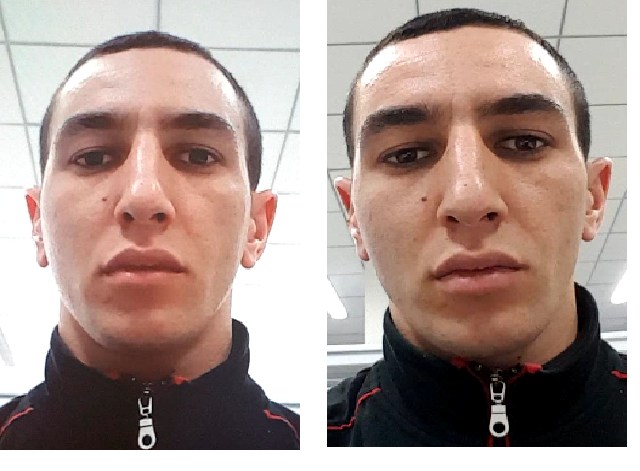
\includegraphics[width=\linewidth]{realAndFakeEx}}
	\caption{نمونه‌ای از تصاویر واقعی و تقلبی در حوزه چهره \cite{boulkenafet2017oulu}}
	\label{fig:realandfake}
\end{figure}

\section{اهداف}
در این پایان‌نامه برای کشف تقلب در تصویر چهره، تمرکز بر روش‌هایی است که تنها از تصویر رنگی به‌عنوان ورودی استفاده می‌شود. این رویکرد موجب کاهش هزینه سیستم و قابل استفاده بودن بیشتر خواهد شد. همچنین از انواع حمله‌های مختلف موجود، تنها موارد چاپ روی کاغذ و بازپخش ویدیو بررسی می‌گردد. با آن‌که حمله‌های دیگری نظیر استفاده از ماسک سه بعدی نیز وجود دارد اما اعمال چنین حمله‌هایی هزینه‌بر و دشوارتر از نظر اجرا است. بنابرین توجه پایان‌نامه روی حملاتی است که متداول‌تر و بیشتر قابل اجرا است. در این پایان‌نامه با ترکیب روش کلاسیک بینایی ماشین و روش‌های جدید یادگیری عمیق ساختاری برای طبقه‌بندی دقیق‌تر ارائه شده است. این ساختار شامل یک عملگر جدید است که از عملگر LBP کلاسیک الهام گرفته شده است، با این تفاوت که این عملگر همانند عملگر کانولوشن در شبکه‌های عمیق دارای پارامتر برای یادگیری عملگر بهینه با توجه به داده‌های ورودی است. همچنین دو تابع هزینه جدیدی ارائه شده است که هدف آن افزایش دقت و تعمیم‌پذیری شبکه روی داده‌های آزمون دیده نشده است.
\section{دستاورد‌های پژوهش}
در این پایان‌نامه نشان داده می‌شود روش ارائه شده شامل عملگر تحلیل ریزبافت و تابع هزینه جدید موجب افزایش دقت طبقه‌بندی و تعمیم پذیری آن می‌شود. همچنین برای پیاده‌سازی، برنامه‌نویسی به زبان پایتون انجام شده است و ملاحظات پیاده‌سازی و چالش‌های مربوط به آن، توضیح و تفسیر شده است. علاوه بر این، برای کار کردن با داده‌های ویدیویی و استفاده از آن، الگوریتمی ارائه شده است که روند آموزش شبکه را تسریع ببخشد. کدهای مرتبط با برنامه در یک مخزن گیت‌هاب
\LTRfootnote{\href{https://github.com/meysamshahbazi/fas}{https://github.com/meysamshahbazi/fas}}
 به‌صورت متن‌باز منتشر شده است. برنامه به‌گونه‌ای نوشته شده است که نتایج آن قابل بازتولید باشد.
\section{ساختار پایان‌نامه}
در فصل دو، ابتدا مروری بر پژوهش‌های انجام شده در حوزه کشف تقلب انجام می‌شود. تحقیقات انجام شده در این حوزه بسیار وسیع است و تنها به مرور روش‌هایی که اهمیت بیشتر در ادبیات موضوع و روش‌هایی که رویکرد مشابهی با این پایان‌نامه داشته‌اند پرداخته می‌شود. در فصل سه، روش پیشنهادی به‌صورت مبانی نظری گفته می‌شود و در فصل چهار، ابتدا ملاحظات پیاده‌سازی روش ارائه شده بیان می‌گردد و سپس با استفاده از معیارهای ارزیابی متداول در این حوزه، به بررسی دقت روش پیشنهادی پرداخته می‌شود. فصل آخر به نتیجه گیری و بحث در مورد روش پیشنهادی می‌پردازد.


		% فصل اول: مقدمه
% !TeX root=../main.tex

\chapter{مروری بر مطالعات انجام شده}
%\thispagestyle{empty} 
\section{مقدمه}
این فصل به مروری بر برخی از مهم‌ترین روش‌های موجود در حوزه کشف تقلب می‌پردازد. در ابتدا دسته‌بندی کلی برای حل مسئله کشف تقلب ارائه می‌شود و سپس دامنه تمرکز روی یک شاخه از این روش‌ها محدود می‌گردد. هرچند که امروزه استفاده از روش‌های یادگیری عمیق گسترش فراوان یافته است و در بسیاری از مسائل بینایی ماشین، روش‌های کلاسیک منسوخ شده‌اند؛ اما این از اهمیت روش‌های کلاسیک نمی‌کاهد.
روش‌های کلاسیک بینایی ماشین در مقایسه با روش‌های مبتنی بر یادگیری عمیق، از آنجا که تمرکز بیشتری روی الگوریتم تا تمرکز روی استفاده از داده داشته‌اند، می‌توانند دید میدانی خوبی از نزدیک شدن به مسئله بدهند.


در این پایان‌نامه سعی شده است که از این دید کلاسیک برای حل مسئله با بهره گرفتن از ابزارهای یادگیری عمیق استفاده شود. پس در این فصل ابتدا روش‌های کلاسیک مورد بررسی قرار می‌گیرند و سپس مروری بر روش‌های مبتنی بر یادگیری عمیق انجام می‌گیرد. 
همانطور که در شکل 
\ref{fig:algs}
مشخص است روش کلی الگوریتم‌های کشف تقلب و به‌طور کلی بسیاری از مسائل بینایی ماشین ابتدا استخراج ویژگی از تصویر یا ویدیوی ورودی است و سپس طبقه‌بندی ویژگی‌های به‌دست آمده است. استخراج ویژگی نقش مهمی در دقت طبقه‌بندی خواهد داشت. یک استخراج ویژگی، یک تابع از تصویر ورودی به یک بردار است و زمانی استخراج ویژگی به‌درستی انجام گرفته است که بردار خروجی شامل اطلاعات اساسی و مهم برای طبقه‌بندی صحیح باشد.

تفاوت عمده الگوریتم‌های کلاسیک و یادگیری عمیق در قسمت استخراج ویژگی است. بدین صورت که در روش‌های کلاسیک، ویژگی‌ها با استفاده از یک روش ایستا انتخاب می‌شوند ولی در روش‌های شبکه عصبی عمیق با استفاده از بهینه‌سازی یک تابع هزینه، روی داده‌های آموزش، استخراج ویژگی‌های مد نظر یاد گرفته می‌شوند.

\begin{figure}[ht]
\begin{tikzpicture}
	\tikzstyle{connection}=[ultra thick,every node/.style={sloped,allow upside down},draw=\edgecolor,opacity=0.7]
	\node[canvas is zy plane at x=0] (temp) at (-3,0,0)
	{
\includegraphics[width=2cm,height=2cm]{1_1_09_2f_37.png}};
	
	\draw [color=black]
	(temp) node[anchor=south] at (-3,-2){\texttt{Input Face}};
	%\draw[connection] 
	\draw[->,thick] (-2.5,0) -- (-2,0);
	
	\node[trapezium,
	draw = blue!80,
	text = black,
	fill = teal!20,
	rotate=270,
	trapezium stretches = true,
	minimum width = 2cm, 
	minimum height = 3cm] (t) at (-.5,0) {Feature Extraction};
	
	\draw[->,thick] (1.2,0) -- (1.7,0);
	
	\node[rectangle,
	draw = magenta!80,
	text = black,
	fill = magenta!20,
	rotate=270,
	trapezium stretches = true,
	minimum width = 2cm, 
	minimum height = 2cm] (t) at (3,0) {Classification};
	
	%\pic[shift={(1.5,0,0)}] at (4,0) {Ball={name=elt1,%
	%		fill=\SumColor,opacity=0.6,%
	%		radius=3,logo=1/0?}};
	
\end{tikzpicture}
\caption{ساختار کلی الگوریتم‌های کشف تقلب در چهره}
\label{fig:algs}
\end{figure}

در روش‌های کلاسیک، با استفاده از الگوریتم‌های بینایی ماشین، سعی در یافتن یک مؤلفه‌ی مفید از تصویر است که به یافتن علائم مربوط به تقلب در تصویر کمک کند. روش‌های کلاسیک به دو دسته سخت‌افزاری و نرم‌افزاری تقسیم می‌شوند.
\cite{ramachandra2017presentation}


در روش‌های سخت‌افزاری یا از یک سخت افزار خاص استفاده می‌شود، یا از یک تعامل فیزیکی با کاربر نظیر چشمک زدن و یا پاسخ به یک چالش استفاده می‌گردد.
در حالت استفاده از سخت افزار خاص، یک دوربین حرارتی یا چند طیفی به کار برده می‌شود. در این حالت تمایز بین تصویر صورت واقعی و یک کاغذ از طریق بررسی طیف نوری یا حرارت مشخص می‌گردد. در حالت‌های دیگر از کاربر خواسته می‌شود یک سری کلمات را ادا کرده1 یا با دست خود حرکت خاصی را انجام دهد.
لازم به ذکر است که در روش‌های سخت افزاری، قسمت نرم‌افزار حذف نمی‌شود و پردازش‌ها به‌صورت خاص متناسب با سخت‌افزار در خواهند آمد. این بدین معنی است که استفاده از سخت‌افزار، طراحی الگوریتم را حذف نخواهد کرد، بلکه نوع الگوریتم، خاص منظوره بر اساس سخت‌افزار مورد استفاده خواهد شد.
مشکل روش‌های سخت‌افزاری این است که هزینه اضافی دارد و تعامل بیشتر کاربر با سیستم را تحمیل می‌کند. تعامل بیشتر، زمان احراز هویت را طولانی‌تر می‌کند که مطلوب نیست.


در روش‌های نرم‌افزاری از سخت افزار اضافه‌ای استفاده نمی‌شود؛ و تنها از همان دوربین معمولی، تصویربرداری صورت می‌گیرد؛ اما از یک الگوریتم هوشمند بر پایه‌ی بینایی ماشین استفاده خواهد شد. روش‌های نرم‌افزاری به دو دسته ایستان و پویا تقسیم می‌شود.
در روش‌های ایستان، پردازش تنها روی یک فریم تصویر انجام می‌شود و تقلب را با اطلاعات تک تصویر بررسی می‌کند؛ هر چند که این روش‌ها را در دنباله ویدیویی نیز می‌توان به کار برد و روی هر فریم، این پردازش صورت بگیرد. این روش‌ها هزینه محاسباتی کمتری در مقایسه با روش‌های پویا دارند. روش‌های ایستان به سه دسته تحلیل ریزبافت1، تحلیل فرکانس و روش ترکیبی تقسیم می‌شود.
در تحلیل ریزبافت از الگوهای بافت تصویر استفاده می‌شود. این الگوها در مقیاس ذره بینی بررسی می‌گردند. معروف‌ترین عملگر برای این تحلیل عملگر الگوهای دودویی محلی2 (LBP) است که با جزئیات در ادامه توضیح خواهد داده شد.
در روش تحلیل فرکانسی بر اساس تبدیل فوریه و تحلیل مولفه‌های فرکانسی صورت می‌گیرد و شامل استفاده از فیلتر تفاضلی گوسی و تبدیل کسینوسی می‌شود.
در روش‌های پویا از اطلاعات فریم‌های متوالی نیز در کنار هم استفاده می‌شود و برای تحلیل، وابستگی فریم‌های متوالی بررسی می‌شود. در مقایسه با روش‌های ایستان زمان پردازش بیشتری دارند اما دقت بهتری را ارائه می‌کنند. روش‌های پویا به سه دسته تحلیل حرکت، تحلیل بافت و روش‌های ترکیبی تقسیم می‌شود.
در روش پویا از حرکت عضلات صورت به‌وسیله حرکت سر، دهان و چشم بهره برده می‌شود. الگوریتم‌های مورد استفاده در این در بیشتر موارد بر مبنای الگوریتم optical flow است. همچنین روش‌های جداسازی صورت از پس‌زمینه و اطلاعات فرکانسی متحرک نیز مورد استفاده قرار می‌گیرد. همچنین از تغییرات بافت در بین فریم‌های متوالی استفاده می‌شود.
\section{تحلیل ریز بافت و عملگر LBP}
در میان روش‌های نرم‌افزاری ذکر شده، تحلیل ریزبافت در این پایان‌نامه اهمیت بسزایی دارد. یکی از تفاوت‌های بین تصویر واقعی و تقلبی در بررسی بافت اجزای صورت در مقیاس ذره‌بینی1 است. در این مقیاس اثر دانه دانه‌ای چاپ تصویر روی کاغذ منجر به تفاوت با بافت طبیعی چهره انسان نمایان می‌شود. همچنین صورت انسان در مقایسه با تصویر نمایش داده شده روی نمایشگر دیجیتال از نظر بافت پیکسلی متفاوت خواهد بود. همچنین صورت واقعی در مقایسه با تصویر چاپ شده یا نشان داده شده روی نمایشگر دیجیتال از نظر انعکاس نور و بازتاب و تشکیل سایه تفاوت دارد. علاوه بر این‌ها تصاویر تقلبی در مجموع کمی تاری در کیفیت خود دارند. از این رو مسئله کشف تقلب، شباهت‌هایی با مسائل تحلیل کیفیت تصاویر و نهان‌کاوی دارد.

در 
\cite{maatta2011face}
برای اولین بار از عملگر الگوهای دودویی محلی یا به اختصار LBP، در حوزه کشف تقلب در چهره استفاده شده است. این عملگر از تعریف بافت از در یک همسایگی در مقیاس محلی الهام گرفته است و یک توصیف‌گر قوی بافت است. به‌منظور آشنایی اولیه، این عملگر ابتدا در یک پنجره سه در سه تعریف می‌شود و سپس رابطه محاسبه آن به‌صورت کلی تعریف می‌شود. در شکل 
\ref{fig:lbpexm}
مثالی از محاسبه این عملگر در پنجره سه در سه نشان داده شده است.
\begin{figure}[ht]
	\centerline{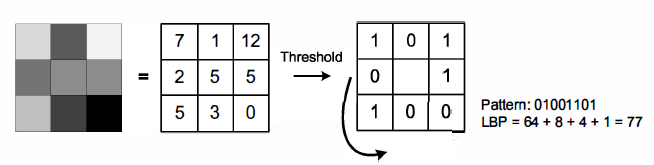
\includegraphics[width=\linewidth]{lbpexm}}
	\caption{مثالی از محاسبه LBP }
	\label{fig:lbpexm}
\end{figure}
ابتدا پیکسل‌های کناری با پیکسل میانی مقایسه می‌شوند، سپس بر مبنای بزرگ‌تر یا کوچک‌تر بودن مقادیر از پیکسل میانی مقدار یک یا صفر به آنها اختصاص داده می‌شود و سپس این دنباله دودویی در یک جهت دایره‌ای خوانده و یک عدد هشت بیتی می‌دهد. در پنجره سه در سه 8 پیکسل مجاور موجود هست و تعداد حالت‌هایی که خروجی عملگر می‌تواند داشته باشد برابر با
$2^8=256$
است.





تعریف رسمی این عملگر به‌صورت کلی برای شعاع R و تعداد نقاط نمونه برداری P در محیط دایره به‌صورت رابطه
\ref{eq:lbpDef}
است.
\begin{equation}\label{eq:lbpDef}
			LBP_{P,R}=\sum_{p=0}^{P-1}s(I_p-I_c)2^p 
\end{equation}

که در آن
$s(.)$
یک تابع غیر خطی است.

\[ s(x) = 
\begin{cases} 1  & \text{$x \geq 0 $}\,; \\
	0  & \text{otherwise}\,.
\end{cases} \]

این رابطه بیان می‌کند برای محاسبه ریزبافت هر پیکسل در هر نقطه ابتدا یک دایره به شعاع R در نظر گرفته و روی محیط آن P نقطه به فواصل مساوی باید انتخاب شود. در صورتی که برخی نقاط انتخاب شده روی پیکسل خاصی قرار نگیرد باید با استفاده از درون‌یابی دو خطی1، مقدار پیکسلی به آن تخصیص داده شود. سپس مقدار این پیکسل‌های روی دایره با پیکسل مرکز دایره مقایسه شده و دنباله دودویی ایجاد می‌گردد. این عمل بدین صورت ادامه می‌یابد که مرکز دایره لغزانده شده و هر بار برای هر پیکسل تصویر ورودی، مقدار LBP محاسبه می‌گردد.

یکی از ویژگی‌های مهم این عملگر، مقاوم بودن در برابر تغییرات یکسان پیکسل‌های تصویر ورودی است. فرض کنید تمامی پیکسل‌ها در یک عدد ثابت ضرب شده یا با یک مقدار ثابت جمع شوند در این صورت به‌علت اینکه خروجی تابع غیرخطی تغییر نخواهد کرد مقدار نهایی خروجی LBP تغییری نمی‌کند.
همچنین این عملگر بار محاسباتی کمی دارد پس سریع است. تفاضل گیریی و اعمال تابع غیر خطی   
$s(.)$
ساده است و اعمال ضریب
$2^p$
به کمک شیفت، قابل انجام است.
\begin{align}\label{eq:lbpfeature}
	&I \to \alpha I \to s(\alpha I_p -\alpha I_c) = s(I_p - I_c) \\
	&I \to I+\beta \to s((I_p + \beta)-(I_c + \beta)) = s(I_p - I_c ) 
\end{align}

یک نسخه تکامل یافته از LBP، نسخه‌ی یکنواخت این عملگر است که با  نشان داده می‌شود. این عملگر از این رو معرفی شده است که برخی از الگوهای دودویی بیشتر از سایرین در تصویر متداول‌اند. یک LBP را یکنواخت گویند اگر حداکثر دو تغییر از صفر به یک یا برعکس در نمایش دودویی آن به‌صورت چرخشی وجود داشته باشد. برای محاسبه برچسب خروجی در حالت یکنواخت، هر الگوی یکنواخت با یک مقدار مجزا نشان داده می‌شود و تمامی حالت‌های غیر یکنواخت به یک مقدار متناظر می‌شوند.

هر خروجی LBP می‌تواند نمایانگر وجود یک نوع الگوی ریزبافت باشد. برای مثال یک LBP با مقدار خاص می‌تواند نشانگر نقطه، گوشه، مسطح و... باشد. پس فراوانی این الگوها در تصویر اهمیت دارد. پس از محاسبه LBP به ازای هر پیکسل تصویر، هیستوگرام آن محاسبه می‌شود و از طریق توزیع فراوانی الگوهای ریزبافت‌های متفاوت موجود در تصویر، در مورد واقعی یا غیر واقعی بودن آن تصمیم گیری می‌شود.
\begin{figure}[hb]
	\centerline{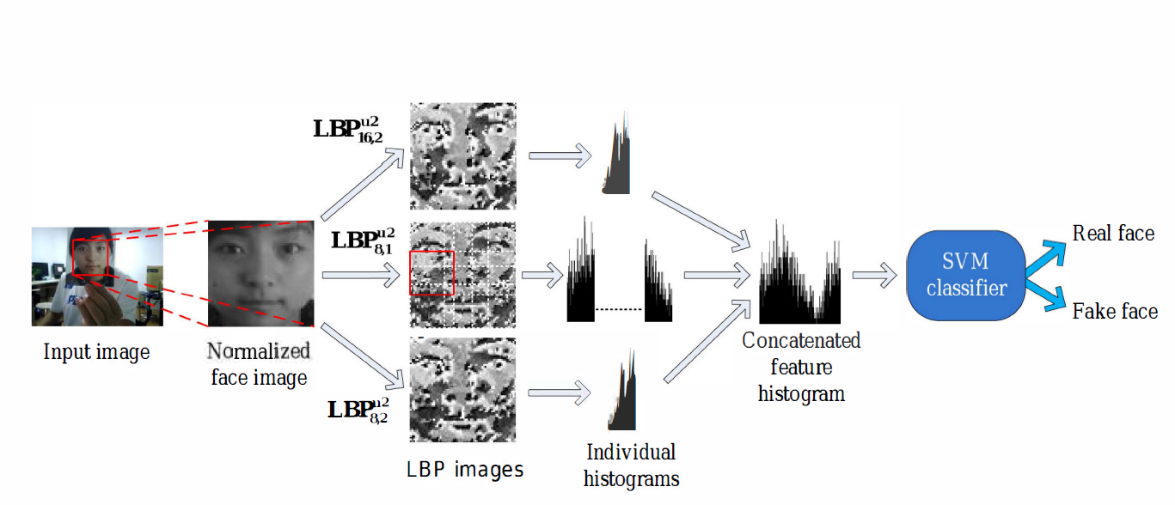
\includegraphics[width=\linewidth]{lbpmatta}}
	\caption{روش تصمیم‌گیری بر اساس استفاده از LBP \cite{maatta2011face}}
	\label{fig:lbpmatta}
\end{figure}

روش محاسبه و تصمیم گیری ارائه شده در 
\cite{maatta2011face}
در مورد واقعی یا تقلبی بودن تصویر چهره با استفاده از تحلیل ریزبافت به‌صورت شکل
\ref{fig:lbpmatta}
است.
ابتدا با استفاده از الگوریتم تشخیص چهره، مختصات صورت انتخاب شده و مقادیر پیکسلی چهره به‌صورت نرمالیزه می‌شود. سپس عملگر LBP با شعاع‌های متفاوت اعمال شده و هیستوگرام آنها محاسبه می‌شود، سپس این هیستوگرام‌ها کنار هم گذاشته می‌شود و با الگوریتم SVM طبقه بندی صورت می‌گیرد.

در 
\cite{chingovska2012effectiveness}
بر خلاف روش قبلی تنها از عملگر LBP یکنواخت در پنجره سه در سه به‌صورت نرمالیزه شده استفاده شده است و از عملگر LBP با شعاع‌های متنوع 
\cite{maatta2011face}
استفاده نشده است. همچنین در 
\cite{chingovska2012effectiveness}
به این نکته پرداخته شده است که باید به ریزبافت در نواحی مختلف صورت توجه داشت و توزیع فراوانی ریزبافت‌ها را نباید صرفاً در کل ناحیه صورت بررسی کرد.
\begin{figure}[t]
	\centerline{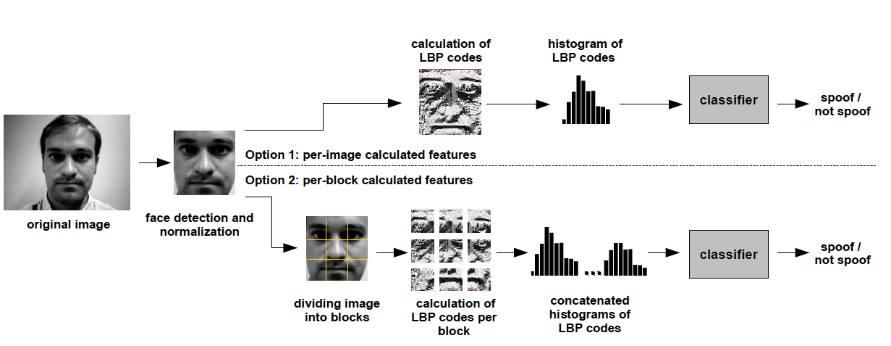
\includegraphics[width=\linewidth]{lbpchin}}
	\caption{روش تحلیل ریزبافت در نواحی مختلف تصویر \cite{chingovska2012effectiveness}}
	\label{fig:lbpchin}
\end{figure}
در این روش در یک حالت هیستوگرام LBP صورت در کل تصویر محاسبه می‌شود؛ در حالت دیگر ناحیه صورت به 9 ناحیه تقسیم شده و در هر کدام به‌صورت جداگانه هیستوگرام LBP محاسبه می‌شود و این هیستوگرام‌ها در کنار هم قرار داده می‌شود. سپس هیستوگرام‌ها به‌عنوان یک بردار ویژگی به طبقه‌بند داده می‌شود. در این روش توزیع هر تصویر با توزیع هیستوگرام تصویر چهره واقعی مقایسه می‌شود این مقایسه به روش X2 histogram comparison انجام می‌گیرد.

دو روش گفته شده از LBP به‌صورت ایستا استفاده کرده‌اند. یعنی ورودی سیستم تنها یک تصویر از چهره فرد است. از آنجا که اطلاعات بین فریم‌ها یعنی تحلیل یک دنباله ویدیویی، می‌تواند به دقت تشخیص کمک کند، پریریا و همکاران عملگر LBP را در فضای سه‌بعدی گسترش داده‌اند تا از اطلاعات بافت در حوزه مکانی تصویر و حوزه زمانی بین فریم‌های متوالی در تصمیم‌گیری استفاده شود
\cite{freitas2012lbp}.
\section{روش‌های مبتنی بر یادگیری عمیق}
 در عملگر LBP انتخاب ویژگی به‌صورت دستی انجام می‌گیرد. انگیزه انتخاب ویژگی به‌صورت هوشمند موجب استفاده از روش‌های یادگیری عمیق برای این کار شده است. ایده استفاده از یادگیری عمیق در حوزه کشف تقلب در تشخیص چهره برای اولین بار توسط ینگ و همکاران مطرح شد 
\cite{yang2014learn}
.
 روش ارائه شده در این کار بدین صورت است که ابتدا صورت تشخیص داده می‌شود و پنجره انتخاب شده برای صورت، به‌گونه‌ای در مقیاس‌های مختلف بزرگ می‌شود که شامل پس زمینه صورت نیز باشد. چرا که اطلاعات پس زمینه نیز می‌تواند به کشف تقلب کمک کند. سپس این تصاویر به یک شبکه ALEXNET
\cite{krizhevsky2012imagenet}
  داده می‌شود و این شبکه کانولوشن ویژگی‌های مد نظر را استخراج می‌کند و در انتها به‌وسیله SVM طبقه‌بندی صورت می‌گیرد.با اینکه این کار در سال 2014 انجام شده است، اما کاشف به عمل آمده است که استفاده خام از شبکه عصبی عمیق به تنهایی نمی‌تواند به دقت مطلوب برسد. به همین دلیل تاکنون پژوهش‌ها در این حوزه ادامه داشته است و ایده‌های مختلفی برای بهبود عملکرد و افزایش دقت طبقه‌بندی مطرح شده است. 
 
 روش گفته شده روی یک فریم کار می‌کند. برای بهره بردن از اطلاعات بین فریم‌های مختلف استفاده از کانولوشن سه بعدی پیشنهاد شده است 
\cite{gan20173d,li2018learning}
 . شیوه دیگر برای کمک گرفتن اطلاعات فریم‌های متوالی استفاده از ساختار
LSTM \cite{hochreiter1997long}
  پس از شبکه کانولوشن است که کارهای
\cite{xu2015learning,yang2019face}
از این ساختار استفاده کرده‌اند.
 

\subsection{ترکیب روش‌های یادگیری عمیق و ویژگی‌های دستی}
یک ایده برای افزایش دقت شبکه عصبی پیشنهاد ترکیب ویژگی‌های لایه‌های کانولوشن با ویژگی‌های دستی1 است. نمای کلی حالت مختلفی که می‌توان برای این کار، ساختار ارائه کرد در شکل 
\ref{fig:cnn-hand}
نشان داده شده است 
\cite{yu2021deep}
 حالت‌های مخلتف این روش بدین صورت است که می‌توان ابتدا ویژگی دستی را استخراج کرد و این ویژگی‌ها را به یک شبکه عمیق داد. یا می‌توان ابتدا از شبکه عمیق برای استخراج ویژگی استفاده کرد و سپس روی ویژگی‌های عمیق به‌دست آمده از روش‌های استخراج ویژگی دستی استفاده کرد یا آنکه ویژگی‌های عمیق و ویژگی‌های دستی را با هم ادغام کرده و سپس به طبقه‌بند داده شود.

\begin{figure}[t]
	\centerline{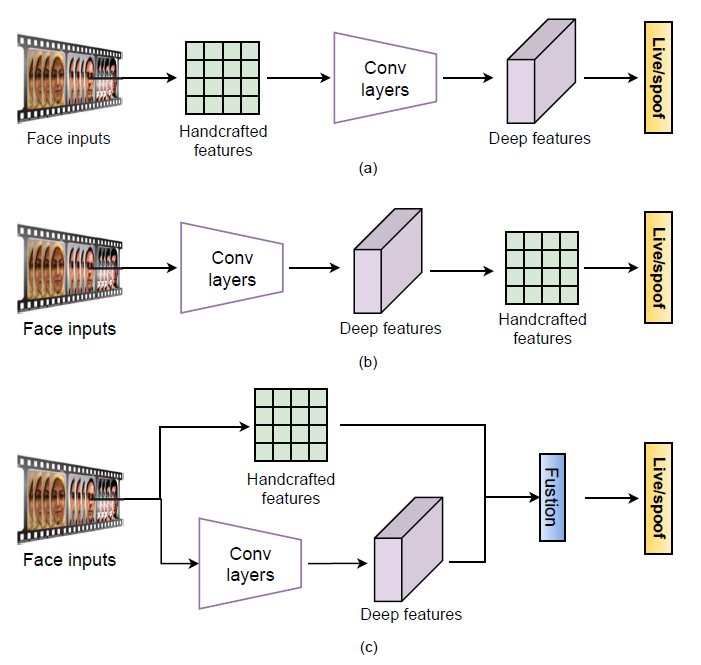
\includegraphics[width=0.5\linewidth]{cnn-hand}}
	\caption{حالت‌های مختلف ترکیب ویژگی‌های دستی و ویژگی‌های یادگیری عمیق \cite{yu2021deep}}
	\label{fig:cnn-hand}
\end{figure}

برای مثال فنگ و همکاران 
\cite{li2016original} 
پیشنهاد داده‌اند که از شبکه‌ی از قبل آموزش داده شده استفاده شود. بدین صورت که از شبکه
 VGG-face \cite{parkhi2015deep}
 که برای تشخیص چهره، روی حجم زیادی داده آموزش داده شده است، استفاده می‌شود و این شبکه روی داده‌های مربوط به کشف تقلب، تنظیم دقیق1 می‌گردد. در مرحله بعد از وزن‌های بهبود یافته استفاده می‌شود و تصاویر نمونه به شبکه داده می‌شود و سپس مقادیر لایه‌های میانی شبکه، به‌صورت ماتریسی روی هم قرار داده می‌شوند و میانگین گرفته می‌شود سپس مقادیری که مقدار زیادی دارند نگه داشته می‌شوند و بعد آن‌ها با الگوریتم PCA کاهش داده می‌شود. سپس ماتریس کاهش بعد داده شده به یک طبقه بند SVM داده می‌شود و تصمیم‌گیری انجام می‌شود. 

لی و همکاران ابتدا یک شبکه عصبی VGG-face را روی داده‌های مربوط به تشخیص تقلب تنظیم دقیق کرده‌اند و سپس روی کانال‌های مختلف در لایه‌های شبکه، عملگر LBP را اعمال کرده‌اند. با گرفتن هیستوگرام روی آن از SVM برای طبقه بندی استفاده کرده‌اند
\cite{li2019face}.
رحمان و همکاران روی تصویر ورودی عملگر LBP زده‌اند و با ترکیب ویژگی‌های لایه اول کانولوشن و خروجی LBP را به ادامه شبکه عصبی داده‌اند
\cite{rehman2020enhancing}. 
 این ایده در شکل
\ref{fig:rahman}
نشان داده شده است.

روش‌های ترکیبی بین ویژگی‌های دستی و ویژگی‌های یادگیری عمیق دارای یک قسمت ایستا هستند که حین آموزش شبکه تغییری نخواهند کرد. برای روش‌های مبتنی بر شبکه عصبی مطلوب این است که تمامی قسمت‌های شبکه به‌صورت انتها به انتها یاد گرفته شود.
\begin{figure}[hb]
	\centerline{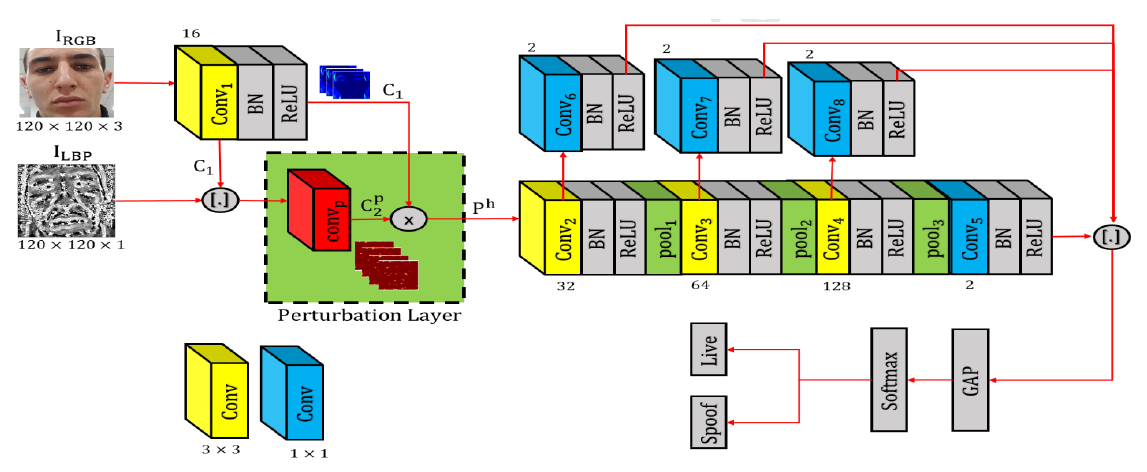
\includegraphics[width=0.5\linewidth]{rahman}}
	\caption{روش ترکیب LBP و کانولوشن \cite{rehman2020enhancing}}
	\label{fig:rahman}
\end{figure}

\subsection{استفاده از تخمین سیگنال کمکی}
در روش‌های بیان شده روال آموزش شبکه عصبی بهینه کردن تابع هزینه آنتروپی متقاطع دودویی1 است. با این رویکرد که در انتهای شبکه یک نورون برای تصمیم‌گیری وجود دارد و تابع هزینه روی این نورون اعمال می‌شود. مشکل این روش این است که شبکه ممکن است ویژگی‌های غیر مطلوبی را پیدا کند که هر چند در جداسازی داده‌های آموزش مفید است اما ممکن است مشابه این ویژگی‌ها در داده‌های آزمون وجود نداشته باشد. این مشکل با عنوان بیش‌برازش2 در علم یادگیری ماشین شناخته می‌شود.

\begin{figure}[h]
	\centerline{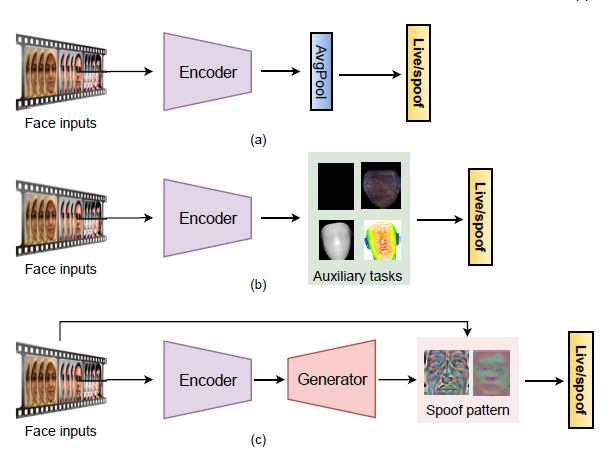
\includegraphics[width=0.7\linewidth]{cnn-aux-methods}}
	\caption{روش‌های مختلف یادگیری عمیق در حوزه‌ی کشف تقلب چهره \cite{yu2021deep}}
	\label{fig:cnn-aux-methods}
\end{figure}

برای مثال ممکن است شبکه در حین آموزش به قاب صفحه نمایشی که برای حمله استفاده شده است توجه کند، اما در داده‌های آزمون مشابه این قاب وجود نداشته باشد. بدین منظور تلاش محققان برای یافتن ویژگی‌های خوش‌ساخت1 به ایده نظارت کمکی2 رسانده است
\cite{liu2018learning}.  
در روش‌های نظارت کمکی سعی می‌شود از تخمین یک مورد کمکی برای استنتاج تقلبی یا واقعی بودن چهره استفاده شود. یکی از موارد مهم کمکی در این حوزه تخمین عمق صورت است.


به‌طور کلی روش دقیق برای محاسبه عمق، استفاده از دوربین مخصوص است که برای هر پیکسل مقدار متناظر با عمق آن پیکسل را نیز بدهد. همچنین با استفاده از روش‌های سه‌بعدی‌سازی و استفاده از حداقل دو دوربین، بازسازی مدل سه‌بعدی امکان پذیر است. اما در کشف تقلب در حالت نرم‌افزاری مطلوب این است که این کار به وسیله‌ی تنها یک دوربین ساده انجام شود. لذا در این حالت تنها می‌توان تخمینی از عمق را داشت.


استفاده از عمق از این شهود گرفته شده است که مغز انسان چهره واقعی را دارای عمق می‌بیند، برای مثال بینی نزدیک‌تر از گونه‌ها است، اما چهره تقلبی که روی صفحه نمایش یا کاغذ چاپ شده قرار دارد دارای عمقی مسطح است. در روش‌هایی که از عمق به‌عنوان یک سیگنال کمکی استفاده کرده‌اند، پیش از آموزش شبکه کشف تقلب، از یک شبکه تخمین عمق مثل 
PRNet \cite{feng2018joint} 
استفاده می‌شود. و عمق به‌دست آمده را بین صفر و یک نرمالایز می‌شود. برای تصاویر واقعی این تصویر به‌عنوان عمق ذخیره شده و برای تصاویر تقلبی، عمق مسطح صفر در نظر گرفته می‌شود. اکنون از این برچسب عمق برای آموزش ساختار شبکه عصبی توسعه داده شده استفاده می‌شود
\cite{atoum2017face,yu2020searching,shao2019multi,liu2018learning,wang2020deep,wang2018exploiting}.
\begin{figure}[h]
	\centerline{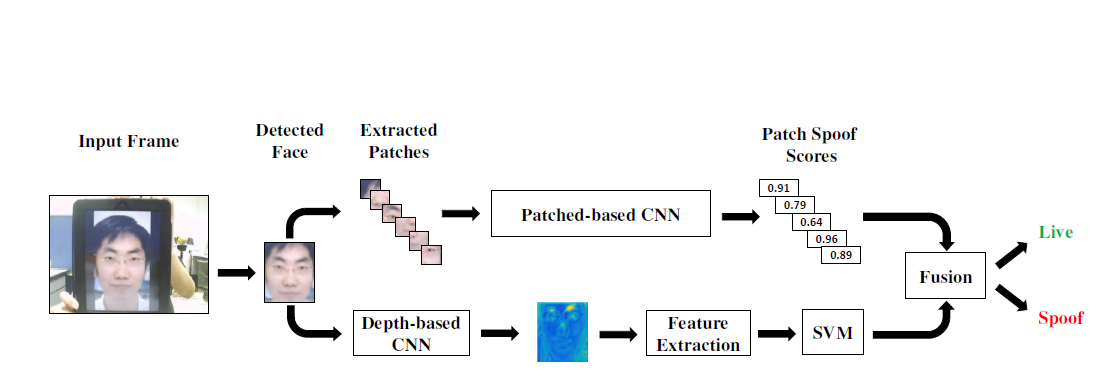
\includegraphics[width=\linewidth]{cnn-depth}}
	\caption{استفاده از عمقب برای کشف تقلب در چهره  \cite{atoum2017face}}
	\label{fig:cnn-depth}
\end{figure}

اتوم و همکاران
\cite{atoum2017face}
  برای اولین بار در این حوزه از عمق به‌عنوان سیگنال کمکی استفاده کرده‌اند. روش ارائه شده بدین صورت است که ابتدا از تصویر ورودی، صورت تشخیص داده شده و تصویر صورت به دو شبکه داده می‌شود. در مسیر بالایی شکل
\ref{fig:cnn-depth}
   قسمت‌های مختلف صورت به‌صورت تصادفی انتخاب شده و به یک شبکه عصبی کانولوشنی داده می‌شود و در مسیر پایین از طریق یک شبکه عصبی، عمق تصویر تخمین زده می‌شود. سپس اطلاعات دو مسیر با یکدیگر ترکیب شده و در مورد واقعی یا غیرواقعی بودن تصویر تصمیم‌گیری می‌شود.
   
   همچنین لیو و همکاران
\cite{liu2018learning}
   علاوه بر استفاده از سیگنال کمکی عمق از تخمین سیگنال rPPG در طول فریم‌های متوالی به‌عنوان سیگنال حیات چهره بهره برده‌اند. در قسمت عمق مشابه
\cite{atoum2017face}
   ابتدا برچسب عمق واقعی برای چهره زنده و عمق صفر برای چهره تقلبی تخمین زده شده و از تابع هزینه رابطه
\ref{eq:depthreg}
   برای بهینه سازی شبکه استفاده می‌شود. که در آن  عمق متناظر با تصویر  است.
\begin{equation}\label{eq:depthreg}
	\Theta_D = \argmin_\Theta{\sum_{i=1}^{N_d}||CNN_D(I_i;\Theta)-D_i||^2_1} 
\end{equation}

\begin{figure}[t]
	\centerline{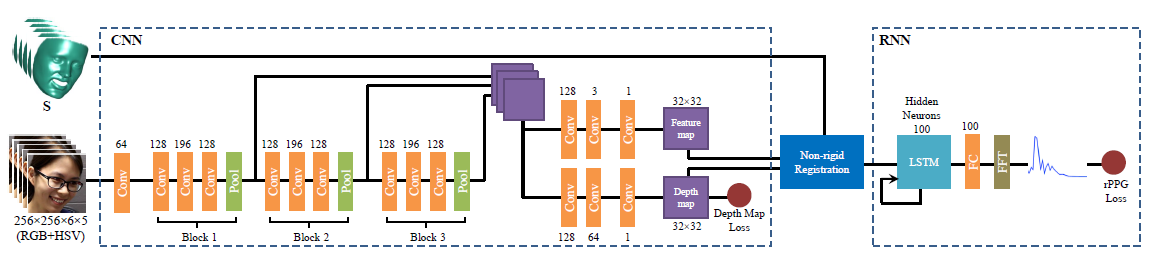
\includegraphics[width=\linewidth]{depth-rppg}}
	\caption{روش استفاده از عمق و تخمین rPPG \cite{liu2018learning}}
	\label{fig:depth-rppg}
\end{figure}

همچنین ونگ و همکاران
\cite{wang2018exploiting}
ساختاری را به کمک optical flow روی ویژگی‌های شبکه عصبی برای تخمین عمق توسعه داده‌اند، به‌گونه‌ای که اطلاعات حرکتی بین فریم‌های متوالی نیز در نظر گرفته می‌شود. همچنین از ترکیب ساختار
 GRU \cite{cho2014learning}
با کانولوشن بلوکی به نام ConvGRU معرفی کرده‌اند که در آن در رابطه GRU به‌جای ضرب‌های ماتریسی از عملگر کانولوشن استفاده شده است و کاربرد آن توجه به ویژگی‌های بلند مدت در میان فریم‌های متوالی ورودی است.

\begin{figure}[h]
	\centerline{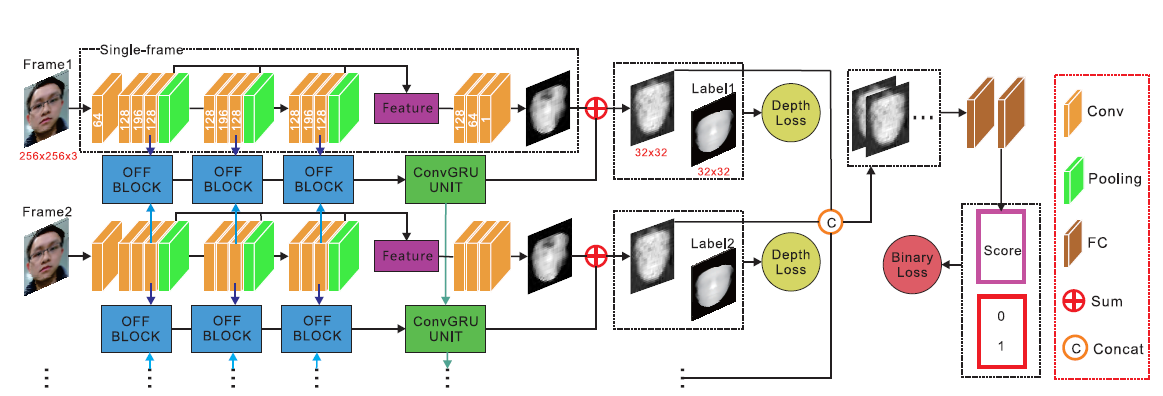
\includegraphics[width=\linewidth]{wang}}
	\caption{استفاده از ویژگی‌های عمیق در طول زمان \cite{wang2018exploiting}}
	\label{fig:wang}
\end{figure}
در استفاده از سیگنال کمکی عمق در شبکه نه تنها مقدار عمق می‌تواند مهم باشد بلکه پیوستگی عمق بین پیکسل‌های مجاور نیز اهمیت دارد. بدین منظور تابع هزینه CDL برای در نظر گرفتن این پیوستگی عمق در پیکسل‌های مجاور توسعه داده شده است
\cite{wang2020deep,wang2018exploiting}
در تابع هزینه CDL به‌جای محاسبه فاصله اقلیدسی عمق تخمینی و برچسب عمق به‌صورت پیکسل به پیکسل مشابه رابطه
\ref{eq:cdl}
، از تفاوت عمق بین پیکسل‌های مجاور نیز استفاده می‌شود.
\begin{equation}\label{eq:cdl}
	L_{CDL} = \sum_{i}||K_i^{CDL} \odot D_P-K_i^{CDL} \odot D_G||
\end{equation}
که در آن
$D_P$
عمق تخمین زده شده توسط شبکه و
$D_G$
عمق برچسب واقعی است و
$K_i^{CDL}$
هسته‌های کانولوشن دارای 0 و 1 و-1 هستند که در شکل
\ref{fig:cdl}
نشان داده شده است. و  نشانگر عملگر کانولوشن است. در شکل
\ref{fig:cdl}
مربع بنفش متناظر با عدد 1- و مربع زرد متناظر با عدد 1 و مربع‌های سفید عدد 0 را در هسته نشان می‌دهند. 
 \begin{figure}[ht]
 	\centerline{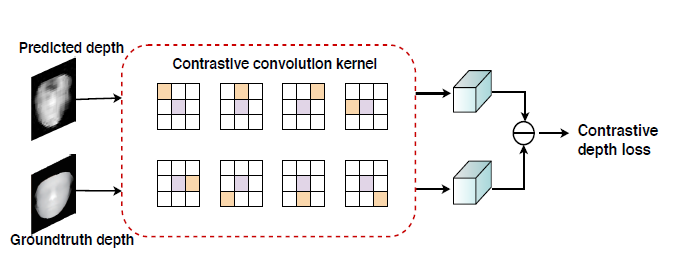
\includegraphics[width=0.5\linewidth]{cdl}}
 	\caption{نحوه محاسبه تابع هزینه CDL}
 	\label{fig:cdl}
 \end{figure}
یو و همکاران
\cite{yu2020searching}
ساختاری تغییر یافته از شبکه‌های کانولوشنی با تأکید بر پیکسل مرکزی پنجره کانولوشن توسعه داده‌اند که درشکل
\ref{fig:central-dif}
نشان داده شده است.
این ساختار با الهام از LBP ایجاد شده است، به‌گونه‌ای که در هر بار انجام عملگر کانولوشن، پیکسل مرکزی از پیکسل‌های مجاور کم خواهد شد. که رابطه
\ref{eq:central-dif1}
این عملگر را نشان می‌دهد.
\begin{equation}\label{eq:central-dif1}
	y(p_0) = \sum_{p \in R} w(p_n).(x(p_0+p_n)-x(p_0)) 
\end{equation}
برای آنکه از خاصیت کانولوشن نیز استفاده شود ترکیب خطی رابطه
\ref{eq:central-dif1}
با رابطه کانولوشن حساب می‌گردد.
\begin{equation}\label{eq:central-dif2}
	y(p_0) = \theta\sum_{p \in R} w(p_n).(x(p_0+p_n)-x(p_0)) +
	(1-\theta)\sum_{p \in R}w(p_n).(x(p_0+p_n)
\end{equation}
که در آن
$\theta$
یک هایپر پارامتر است و قسمت اول رابطه
\ref{eq:central-dif2}
کانولوشن تفاضلی مرکزی و قسمت دوم کانولوشن کلاسیک است. این رابطه در نهایت به‌صورت رابطه
\ref{eq:central-dif3}
ساده می‌گردد.
\begin{equation}\label{eq:central-dif3}
	y(p_0) = \sum_{p \in R} {w(p_n).x(p_0+p_n)} +
	\theta(-x(p_0)\sum_{p \in R}{w(p_n)}
\end{equation}
\begin{figure}[h]
	\centerline{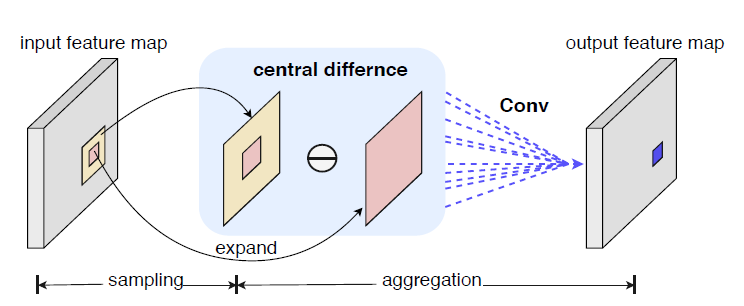
\includegraphics[width=0.5\linewidth]{central-dif}}
	\caption{عملگر کانولوشن تغییر یافته \cite{yu2020searching} }
	\label{fig:central-dif}
\end{figure}

که همانطور که مشاهده می‌شود که همان کانولوشن کلاسیک خواهد بود که پیکسل مرکزی وزن متفاوتی نسب به کانولوشن کلاسیک خواهد داشت. از این ساختار برای تخمین سیگنال کمکی عمق با نظارت تابع هزینه CDL کمک استفاده می‌شود. همچنین برای یافتن اندازه‌ی شبکه از روش جستجوی معماری شبکه1 
\cite{zoph2016neural}
استفاده شده است.

در جستجوی معماری شبکه بر خلاف روش‌های کلاسیک که طراحی معماری شبکه با مهندسی و سعی و خطا انجام می‌شود، تلاش می‌شود معماری بهینه برای کاربرد مورد نظر به‌صورت خودکار با یادگیری تقویتی و مفاهیم یادگیری ماشین پیدا شود. در حوزه کشف تقلب علاوه بر
\cite{zoph2016neural}
کارهای
\cite{yu2020fas,yu2020auto} 
متدهایی بر پایه این ابزار برای یافتن شبکه بهینه پیشنهاد داده‌اند.
 
 لی و همکاران به‌جای تخمین عمق در یک صفحه دو بعدی، از ابر نقاط در فضای سه‌بعدی به‌عنوان سیگنال کمکی استفاده کرده‌اند و ساختاری به نام 3DPC-NET پیشنهاد کرده‌اند
\cite{li20203dpc}.
 
 یو و همکاران 
\cite{yu2020face}
 مسئله تشخیص تقلب در چهره را یک مسئله تشخیص ماده فرض کرده‌اند. این فرض با توجه به این واقعیت استفاده شده است که جنس پوست صورت با جنس کاغذ چاپ‌شده و جنس صفحه‌ی نمایش متفاوت است. برای تشخیص جنس ماده با الهام از فیلتر bilateral روی ویژگی‌های شبکه عمیق از این فیلتر استفاده کرده‌اند. فیلتر bilateral میانگین وزن‌دار روی پیکسل‌های مجاور است که با افزایش فاصله تأثیر آن به‌صورتی تابعی گوسی کاسته می‌شود و روی هر پیکسل به مختصات p و تصویر I به‌صورت رابطه 
\ref{eq:bilat}  
 تعریف می‌شود.
\begin{equation}\label{eq:bilat}
	BiBase(I_p)=\frac{1}{k}\sum_{q\in I}{g_{\sigma_s}(||p-q||)g_{\sigma_r}(||I_p-I_q||)I_q}
\end{equation}
\begin{equation}\label{eq:bilat}
	k=\sum_{q\in I}{g_{\sigma_s}(||p-q||)g_{\sigma_r}(||I_p-I_q||)}
	\nonumber
\end{equation}

که در آن
$g_\sigma (x) = \exp(\frac{-x^2}{\sigma^2})$
تابع گوسی است. در این روش ساختار شبکه مشابه
\cite{liu2018learning}
 است ولی روی ویژگی‌های کانولوشن این فیلتر اعمال شده است.
 
\begin{figure}[t]
 	\centerline{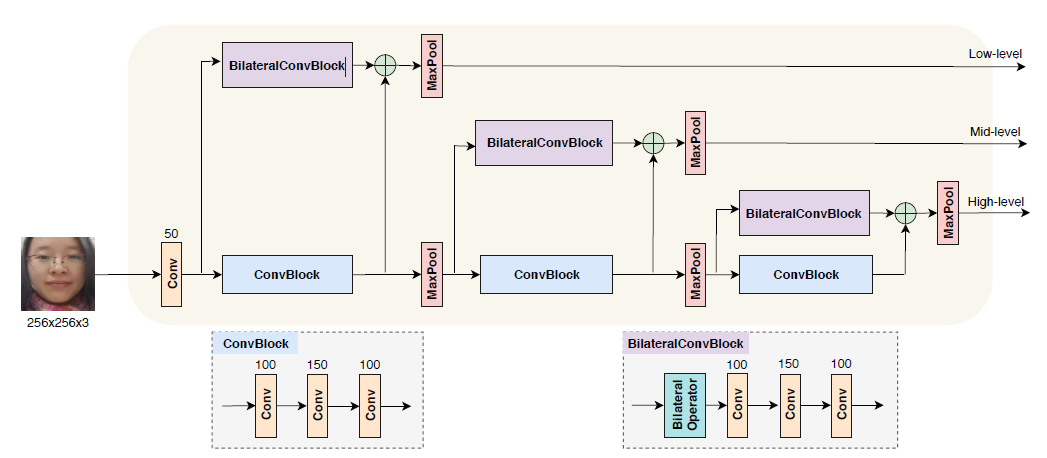
\includegraphics[width=0.7\linewidth]{bilat}}
 	\caption{روش استفاده از فیلتر bilateral در شبکه عمیق \cite{yu2020face} }
 	\label{fig:bilat}
\end{figure}

با وجود آن‌که سیگنال کمکی عمق در ادبیات موضوع به‌طور گسترده استفاده شده است اما پر هزینه است و نیاز به پردازش بیشتر برای تخمین عمق دارد. جدای از آن‌که عمق، یک سیگنال کامل برای تشخیص تقلب نیست و فرض مسطح در نظر گرفتن عمق در چهره‌های تقلبی، فرض همیشه برقرار نیست. برای مثال فرض کنید مهاجم ابزار حمله مثل صفحه نمایش یا کاغذ چاپ شده را به‌صورت مایل قرار دهد در این صورت عمق به‌صورت یکنواخت در همه‌جا صفر نخواهد بود.

 جرج و مارسل روشی را برای پیدا کردن ویژگی‌های خوش‌ساخت بدون استفاده از عمق پیشنهاد کرده‌اند
 \cite{george2019deep}.
 در این روش از چند لایه اول شبکه DENSNET
\cite{huang2017densely}
برای نشان‌کردن تصویر ورودی به یک صفحه 14*14 استفاده کرده‌اند. و قرارداد کرده‌اند که برچسب واقعی به‌جای یک عدد صفر و یک، یک ماتریس دو بعدی به طول کامل صفر یا یک است و تابع هزینه آنتروپی متقاطع دودویی را به‌جای یک نورون روی یک صفحه دو بعدی در نظر گرفته‌اند. با این روش دیگر نیازی به تخمین عمق نخواهد بود.
\begin{figure}[h]
	\centerline{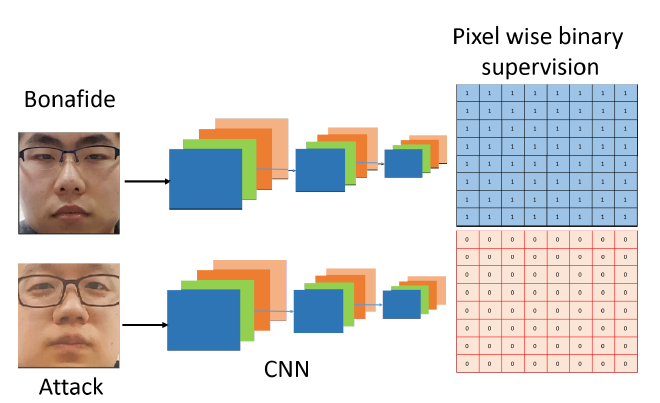
\includegraphics[width=0.5\linewidth]{pixel-wise}}
	\caption{تابع هزینه BCE روی یک صفحه مسطح به‌جای یک نورون \cite{george2019deep} }
	\label{fig:pixel-wise}
\end{figure}
\subsection{استفاده از شبکه‌های مولد تهاجمی و تابع هزینه‌های مختلف}
مسئله کشف تقلب در تشخیص چهره بیشتر شبیه مسئله یافتن یک نویز خاص در تصویر است. ابزارهای حمله نظیر کاغذ چاپ‌شده و صفحه نمایش‌گر، بافت و تفکیک‌پذیری متفاوتی با بافت صورت انسان دارند. که این تفاوت جنس را می‌توان با یک نویز جمع شونده با تصویر چهره انسان زنده مدل کرد. جورابلو و همکاران
\cite{jourabloo2018face}
برای اولین بار مسئله کشف تقلب در چهره از شبکه‌های مولد تهاجمی1 (GAN)
\cite{goodfellow2014generative}
رای مدل کردن و یافتن نویز تصاویر تقلبی استفاده کرده‌اند. با تخمین نویز مربوط به کشف تقلب، قدرت استنتاج برای تقلبی بودن تصویر بیشتر خواهد شد.

از آنجا که نویز مربوط به تقلب می‌تواند در سطوح مختلف در تصویر وجود داشته باشد لیو و همکاران
\cite{liu2020disentangling}
ساختاری بر پایه GAN که الگوهای تقلب در ابعاد مختلف تصویر را تخمین بزند پیشنهاد داده‌اند. در این روش در شبکه مولد dismantlement generator ابعاد تصویر در لایه‌های اول کاهش یافته و سپس افزایش می‌یابد و از ویژگی‌های خروجی لایه‌ها با ابعاد مختلف به‌عنوان ویژگی‌های تقلب تولید شده استفاده می‌شود. در نهایت شبکه multiscale discriminator این ویژگی‌های تقلب در سطوح مختلف را به‌عنوان ورودی دریافت می‌کند و طی یک بازی رقابتی بین دو شبکه در GAN در نهایت ویژگی‌های تقلب بهتری تولید خواهد شد. 
\begin{figure}[h]
	\centerline{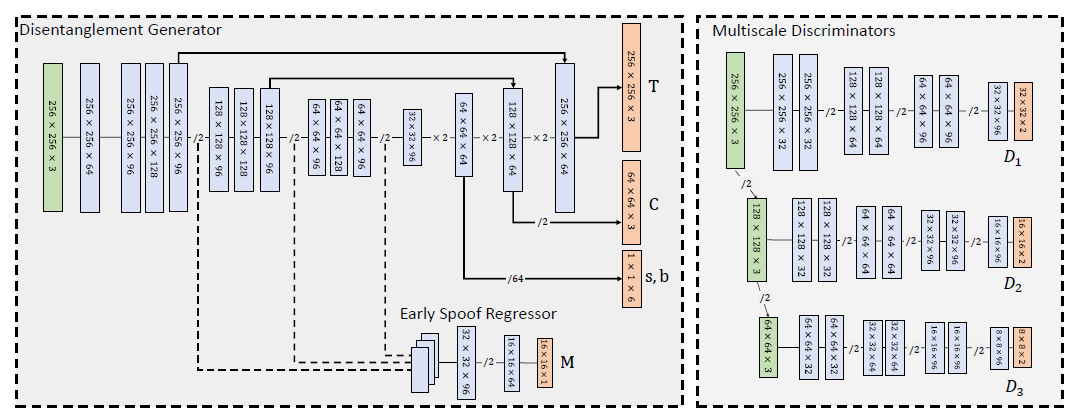
\includegraphics[width=0.7\linewidth]{distang}}
	\caption{ساختار بر پایه استفاده از شبکه مولد برای تخمین علائم تقلب در سطوح مختلف \cite{liu2020disentangling} }
	\label{fig:pixel-wise}
\end{figure}

با وجود اینکه در دو پژوهش اخیر ذکر شده
\cite{jourabloo2018face,liu2020disentangling}
از شبکه مولد تهاجمی برای بهبود دقت در تست درون دیتاست استفاده شده است، توجه پژوهشگران به استفاده از GAN برای تعمیم‌پذیری مدل در دیتاست‌های مختلف جلب شده است
\cite{shao2019multi,jia2020single}.

تعمیم‌پذیری مدل در دیتاست‌های مختلف بدین معناست که برای مثال از بین چهار دیتاست مختلف، سه دیتاست برای آموزش شبکه استفاده می‌گردد و مدل آموزش داده شده روی دیتاست چهارم آزمایش می‌شود. از آنجا که دیتاست‌های مختلف توزیع‌های متفاوتی دارند، رسیدن به دقت خوب در تست روی دیتاست دیده نشده (که توزیع لزوماً یکسانی با توزیع دیتاست‌هایی که برای آموزش استفاده شده است ندارد) یک چالش جدی در این حوزه است. 

همچنین یک روش برای بهبود قابلیت تعمیم‌پذیری، استفاده از تابع هزینه سه‌گانه1 
\cite{schroff2015facenet}
است. در تابع هزینه سه‌گانه هدف این است که استخراج ویژگی به نحوی انجام شود که فاصله ویژگی‌های نمونه‌های مربوط به یک کلاس کوچک و فاصله بین نمونه‌های مربوط به کلاس‌های مختلف زیاد شود.

فرض کنید خروجی شبکه استخراج ویژگی بردار  باشد. در این صورت برای تشکیل تابع هزینه سه‌گانه لازم است که از خروجی‌های شبکه استخراج ویژگی، یک بردار ویژگی لنگر ، یک بردار ویژگی با برچسب یکسان با لنگر  و یک بردار ویژگی با برچسب متفاوت با لنگر   انتخاب شود. تابع هزینه سه گانه به‌صورت رابطه
\ref{eq::tripl}
 تعریف می‌شود.که در آن  یک حاشیه از قبل تعریف شده است. تمام سه‌گانه‌هایی که فاصله درون کلاسی آن‌ها از فاصله برون کلاسی بیشتر از مقدار  است درون مجموع گیری قرار می‌گیرد.که در آن  یک حاشیه از قبل تعریف شده است. تمام سه‌گانه‌هایی که فاصله درون کلاسی آن‌ها از فاصله برون کلاسی بیشتر از مقدار  است درون مجموع گیری قرار می‌گیرد.
 
 \begin{equation}\label{eq:tripl}
L_{trpi} = \sum_{i}{[||f(x_i^a)-f(x_i^p)||_2^2-||f(x_i^a)-f(x_i^n)||_2^2+\alpha]_+}
 \end{equation}

تابع هزینه سه‌گانه به‌صورت رابطه
\ref{eq:tripl1}
نیز قابل بیان است.که در آن زمانی که فاصله درون کلاسی کوچکتر از فاصله برون کلاسی به میزان سطح آستانه  باشد حاصل max صفر خواهد بود و در محاسبات تابع هزینه نقش نخواهد داشت.
 \begin{equation}\label{eq:tripl1}
	L_{trpi} = \sum_{i}{max(0,||f(x_i^a)-f(x_i^p)||_2^2-||f(x_i^a)-f(x_i^n)||_2^2+\alpha)}
\end{equation}

\begin{figure}[t]
	\centerline{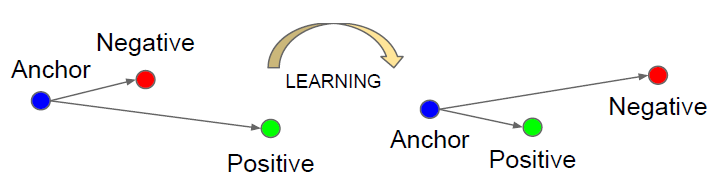
\includegraphics[width=0.7\linewidth]{trip}}
	\caption{نحوه عملکرد تابع هزینه سه‌گانه روی فاصله بردارهای ویژگی \cite{schroff2015facenet} }
	\label{fig:trip}
\end{figure}
شائو و همکاران
\cite{shao2019multi}
از ساختار GAN و ابزار کمکی تخمین عمق و تابع هزینه سه‌گانه برای بهبود تعمیم‌پذیری استفاده کرده‌اند. در این کار یک تابع هزینه بر مبنای تابع هزینه‌ی سه‌گانه توسعه داده شده است که فاصله بین نمونه‌ها با برچسب یکسان در دیتاست‌های مختلف را کوچک‌تر کند و فاصله نمونه‌ها با برچسب متفاوت در یک دیتاست را بیش‌تر کند. با این‌کار توزیع نمونه‌ها در دیتاست‌های مختلف با یک‌دیگر متراکم‌تر خواهد شد. در شکل
\ref{asym} 
به‌کارگیری این تابع هزینه را در بین دو دیتاست مختلف نشان می‌دهد.

\begin{figure}[h]
	\centerline{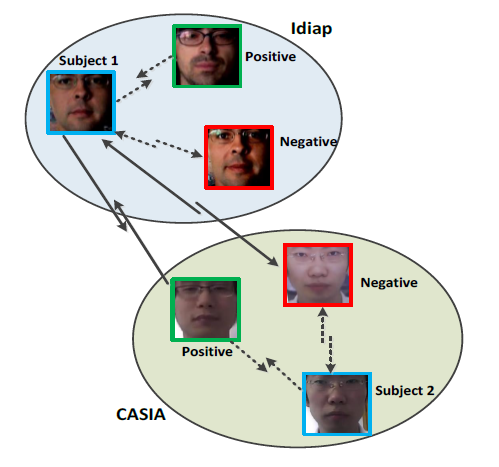
\includegraphics[width=0.4\linewidth]{asym}}
	\caption{نحوه اثر تابع هزینه روی فاصله نمونه‌ها در دیتاست‌های مختلف \cite{shao2019multi} }
	\label{fig:asym}
\end{figure}

همچنین جیا و همکاران
\cite{jia2020single}
 علاوه بر استفاده از GAN صورتی نامتقارنی از تابع هزینه سه‌گانه را پیشنهاد کرده‌اند. به‌گونه‌ای که نمونه‌های زنده در دیتاست‌های مختلف به یک‌دیگر نزدیک‌تر شوند و نمونه‌های تقلبی در دیتاست‌های مختلف از یک دیگر دورتر شده و نمونه‌های واقعی از نمونه‌های تقلبی با فاصله باشند. 
 
 \begin{figure}[h]
 	\centerline{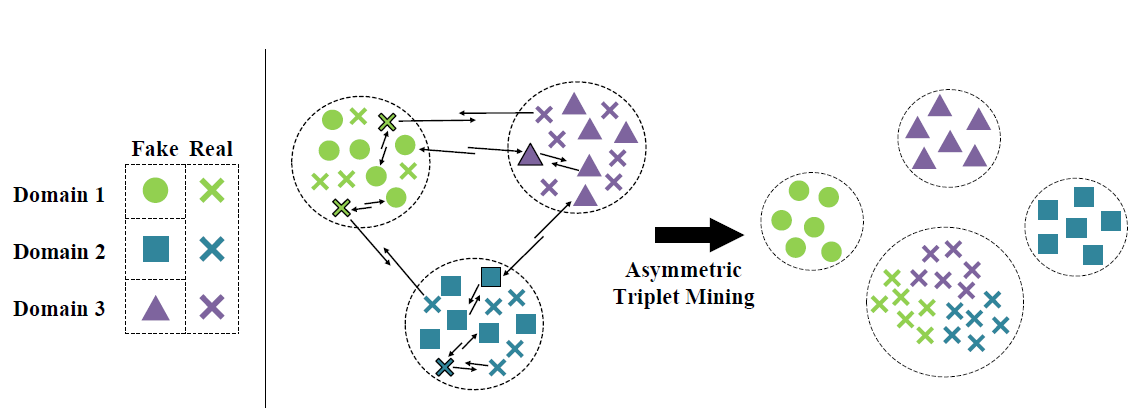
\includegraphics[width=\linewidth]{jia}}
 	\caption{تابع هزینه نامتقارن برای کاهش فاصله نمونه‌های از یک کلاس \cite{jia2020single} }
 	\label{fig:jia}
 \end{figure}

فنگ و همکاران
\cite{feng2020learning}
یک ساختار U-Net
\cite{ronneberger2015u}
به کار برده‌اند و در میان لایه‌های آخر شبکه تولید کننده الگوهای تقلب از تابع هزینه سه‌گانه استفاده کرده‌اند و خروجی این شبکه U-Net را به یک شبکه طبقه بند کمکی داده‌اند.

 \begin{figure}[h]
	\centerline{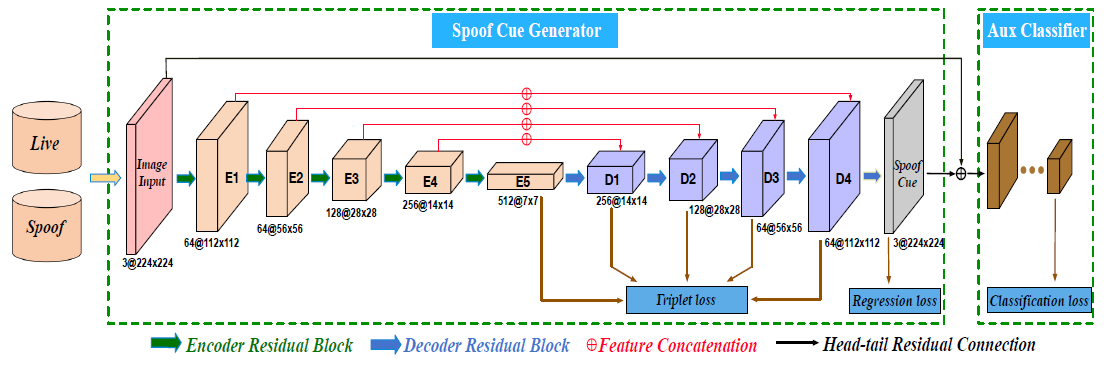
\includegraphics[width=\linewidth]{cue}}
	\caption{ساختار U-net و تابع هزینه سه‌گانه \cite{feng2020learning} }
	\label{fig:cue}
\end{figure}

پرزکابو و همکاران
\cite{perez2019deep}
ابع هزینه سه‌گانه را در فضای نمایی به کار برده‌اند که در رابطه
\ref{eq:ltf}
نشان داده شده است.
 \begin{equation}\label{eq:ltf}
	L_{tf} = \sum_{i}{max(0,e^{\frac{D_{a,p}}{\sigma}}-e^{\frac{D_{a,n}}{\sigma}}+\alpha)}
\end{equation}

که در آن
$D_{a,p}$
فاصله درون‌کلاسی و
$D_{a,n}$
فاصله برون‌کلاسی است و
$\sigma$
یک هایپر پارامتر است.

جرج و مارسل
\cite{george2020learning} 
 تابع هزینه‌ای معرفی کرده‌اند که در فضای n بعدی بردارهای ویژگی، نمونه‌های زنده نزدیک به یک مرکز قرار بگیرند و نمونه‌های تقلبی با یک حاشیه از این مرکز فاصله داشته باشند. مرکز نمونه‌های واقعی در حین آموزش شبکه به‌روزرسانی می‌شود.
فرض کنید مرکز نمونه‌های زنده با  نشان داده شود و فاصله بردار ویژگی نمونه i با مرکز با  تعریف شود. در این صورت تابع هزینه تعریف شده به‌صورت رابطه
\ref{eq:occl}
است.
 \begin{equation}\label{eq:occl}
L_{OCCL}=Y\frac{1}{2}DC^2_W+(1-Y)\frac{1}{2}\max(0,m-DC_W)^2
\end{equation}
که در آن Y برچسب واقعی داده است که برابر با یک است اگر نمونه واقعی باشد و صفر است اگر نمونه تقلبی باشد و m یک حاشیه از قبل تعریف شده است.
 \begin{figure}[h]
	\centerline{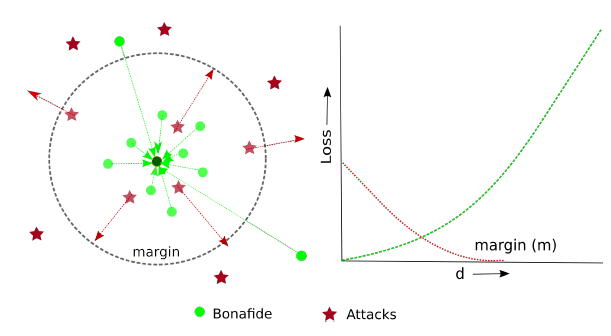
\includegraphics[width=0.5\linewidth]{geo}}
	\caption{کاهش فاصله نمونه‌های واقعی تا مرکز و افزایش فاصله نمونه‌های تقلبی تا مرکز \cite{george2020learning} }
	\label{fig:geo}
\end{figure}

تو و همکاران
\cite{tu2020learning}
 نیز شبکه VGG-face را به‌صورت همزمان با دو هدف شناسایی چهره و تشخیص تقلب آموزش داده‌اند و یک تابع هزینه معرفی کرده‌اند که هدف آن منظم‌سازی1 و جلوگیری از بیش برازش شبکه است. در این تابع فاصله بین هر دو جفت نمونه داده‌ها مستقل از آنکه برچسب آنچه باشد کاهش داده می‌شود. تابع هزینه معرفی شده برای این هدف در رابطه
\ref{eq:tpc}
 بیان شده است. که در آن تابع 
 $\Phi(.)$
  نشان دهنده رابطه بین ورودی تصویر و لایه یکی به آخر شبکه است و M تمام جفت نمونه‌های موجود در دسته آموزش است. 
  \begin{equation}\label{eq:tpc}
 	L_{tpc}=\sum_{i\ne j}^{M}||\Phi(x_i)-\Phi(x_j)||
 \end{equation}

ژنگ و همکاران
\cite{zhang2020face}
علاوه بر تخمین عمق از تخمین LBP به‌عنوان سیگنال کمکی استفاده کرده‌اند که در کنار عمق ساختار LBP تصویر ورودی نیز تخمین زده‌شود. بدین ترتیب که برای تصاویر تقلبی خروجی LBP شبکه باید صفر باشد و برای تصاویر تصاویر واقعی خروجی قسمت LBP باید معادل LBP تصویر ورودی باشد. این شبکه دارای یک شبکه مولد با ساختار U-net و سه شبکه طبقه‌بند برای عمق و LBP و شبکه طبقه بندی بر اساس GAN برای تصویر واقعی و ساختگی است.
 \begin{figure}[h]
	\centerline{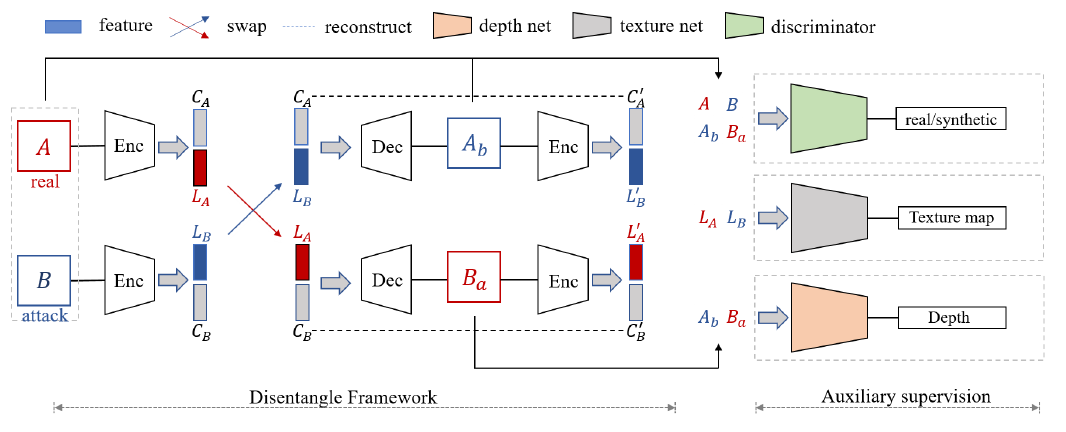
\includegraphics[width=0.7\linewidth]{zhang}}
	\caption{استفاده از LBP در کنار عمق برای یافتن ویژگی‌های خوش ساخت \cite{zhang2020face} }
	\label{fig:zhang}
\end{figure}

ژو و همکاران
\cite{xu2021improving}
روی ثبات فضای ویژگی در بین فریم‌های متوالی یک ویدئو تأکید کرده‌اند. در این کار به‌جای استفاده از الگوریتم‌های تشخیص چهره در هر فریم از الگوریتم دنبال‌کننده‌ی چهره استفاده کرده و چهره‌های تخمین زده شده در فریم‌های متوالی را به شبکه تشخیص تقلب داده‌اند. برای این شبکه تابع هزینه‌ای ارائه معرفی کرده‌اند که فاصله بین بردارهای ویژگی یک ویدئو در دیتاست را کوچک‌تر کند. 
  \begin{equation}\label{eq:xult}
	L_{t}=\frac{1}{m}\sum_{i=0}^{m}\max_{i,j \in v}{||x_i-x_j||^2}
\end{equation}
که در آن m اندازه دسته آموزش است و
$x_i,x_j$
بردارهای فضای ویژگی برای یک ویدئو است. همچنین برای ثبات بردارهای ویژگی در ویدیوهای مختلف، تابع هزینه‌ی دیگری پیشنهاد کرده‌اند که فاصله بین بردارهای ویژگی متعلق به یک برچسب واقعی را نیز کوچک‌تر کند.

  \begin{equation}\label{eq:xule}
	L_{t}=\frac{1}{m}\sum_{i=0}^{m}\max{y_{ij}||x_i-x_j||^2}
\end{equation}

که در آن 
$y_{ij}$
  زمانی که دو بردار ویژگی متعلق به یک کلاس باشند برابر با صفر خواهد بود و در غیر این‌صورت صفر است.
  \section{دیتاست‌های مورد استفاده}
  مانند بسیاری از مسائل بینایی ماشین، دیتاست نقش حیاتی در توسعه الگوریتم و سنجش میزان دقت الگوریتم ایفا می‌کند. از آنجا که تمرکز این پایان‌نامه روی حملات کاغذ چاپ‌شده و بازپخش صفحه نمایش است، به معرفی دیتاست‌هایی که حاوی این نوع حملات هستند پرداخته می‌شود. حملات نظیر استفاده از ماسک، معمولاً براحتی قابل اجرا نیستند و هزینه‌بر هستند اما دو حمله گفته شده از نظر قابلیت اجرا ساده‌تر، کم هزینه و متداول‌تر هستند. 
\subsection{دیتاست Replay}
دیتاست Replay شامل ویدیوهای از 50 شخص مختلف با نمونه‌های واقعی و تقلبی است
\cite{chingovska2012effectiveness}
 نمونه‌های واقعی در شرایط محیطی نوری کنترل‌شده با پس‌زمینه یکنواخت و شرایط محیطی با نور کنترل نشده با پس زمینه غیر یکنواخت گرفته شده‌اند. برای نمونه‌های تقلبی از صفحه کاغذ چاپ‌شده، استفاده از تلفن همراه برای بازپخش ویدئو، و استفاده از تبلت iPAD برای پخش ویدئو با کیفیت بالا استفاده شده است. همچنین نمونه‌های تقلبی در دو حالت استفاده از یک پایه ثابت به‌منظور ثابت ماندن ابزار حمله و استفاده از دست که کمی لغزش خواهد داشت گرفته شده‌اند. رزولوشن تمامی نمونه‌ها واقعی و تقلبی با فرمت QVGA یعنی 320*240 پیکسل است.
\begin{figure}[h]
 	\centerline{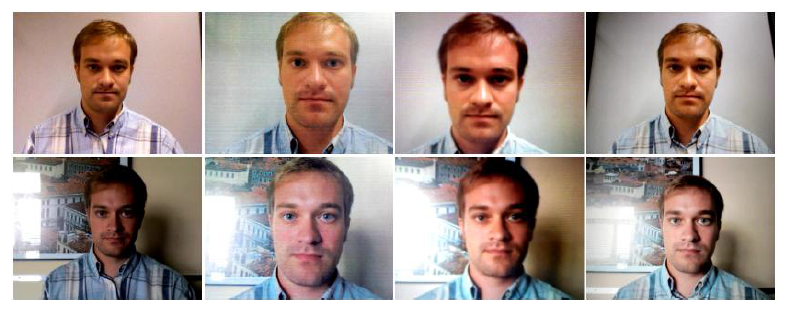
\includegraphics[width=\linewidth]{replay}}
 	\caption{نمونه‌هایی از دیتاست Replay \cite{chingovska2012effectiveness} }
 	\label{fig:replay}
\end{figure}
در
\ref{fig:replay}
نمونه‌هایی از این دیتاست نشان داده شده است. در سطر بالایی نمونه‌ها در محیط کنترل شده از نظر نورپردازی و پس‌زمینه یکنواخت هستند، در حالی که تصاویر سطر پایینی نمونه‌ها دارای نورپردازی غیر کنترل‌شده و پس زمینه غیر یکنواخت هستند. تصاویر از سمت چپ به‌ترتیب تصاویر واقعی، استفاده از کاغذ چاپ‌شده، استفاده از تلفن همراه برای بازپخش و استفاده از تبلت برای بازپخش ویدئو هستند.
\subsection{دیتاست CASIA}
در دیتاست CASIA نیز از 50 شخص مختلف نمونه‌های واقعی و تقلبی گرفته شده است 
\cite{zhang2012face}
. همچنین تصویربرداری با سه نوع دوربین مختلف برای پوشش دادن حالت‌های مختلف در رزولوشن‌های مختلف انجام شده است. در این دیتاست حملات نوع کاغذ چاپ‌شده روی کاغذ گلاسه صورت گرفته است که کیفیت بالاتری نسبت به کاغذ معمولی دارد. همچنین برای حمله بازپخش از تبلت استفاده شده است. در نمونه‌های واقعی دیتاست از کاربر خواسته شده است که پلک و لب بزند تا ویدیوهای ضبط شده دارای اطلاعات حرکتی صورت باشند. در نمونه حمله‌های تقلبی قسمت چشم‌های صورت بریده شده است تا کاربر با پلک زدن بتواند در نمونه‌های تقلبی اطلاعات حرکت به ویدئو بدهد. همچنین در نمونه‌هایی که کاغذ بریده نشده است از کاربر خواسته شده که با حرکت دست کاغذ چاپ شده را حرکت بدهد. نمونه‌هایی از دیتاست CASIA در شکل 
\ref{fig:casia}
نشان داده شده است.

 \begin{figure}[h]
	\centerline{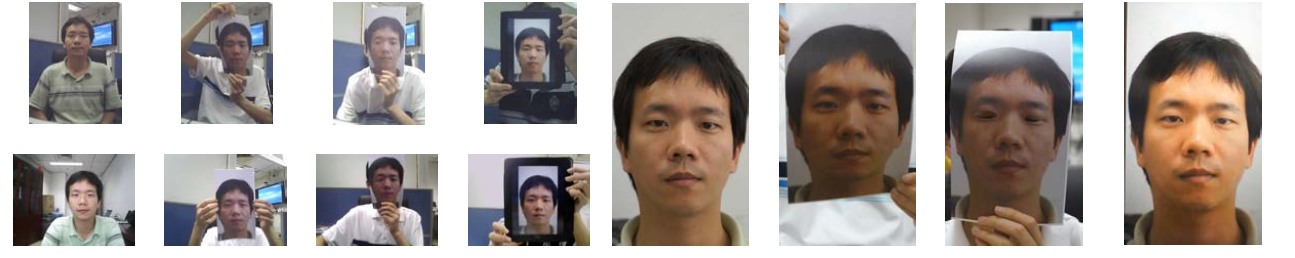
\includegraphics[width=\linewidth]{casia}}
	\caption{نمونه‌هایی از دیتاست CASIA \cite{zhang2012face} }
	\label{fig:casia}
\end{figure}

\subsection{دیتاست MSU}
در دیتاست MSU
\cite{wen2015face}
 از 55 شخص تصویربرداری شده است که ویدیوهای متعلق به 35 فرد در دسترس قرار داده شده است. برای تصویربرداری از دوربین لپ‌تاپ و دوربین تلفن همراه استفاده شده است که دارای رزولوشن 480*640 و 720*480 هستند. استفاده از این نوع دوربین‌ها به‌منظور شبیه‌سازی سناریو احراز هویت از طریق تلفن همراه و لپ‌تاپ انجام شده است. برای حمله باز پخش از صفحه نمایش تبلت و تلفن همراه استفاده شده است. همچنین برای حمله کاغذ چاپ شده از پرینتر با کیفیت استفاده شده است.

 \begin{figure}[h]
	\centerline{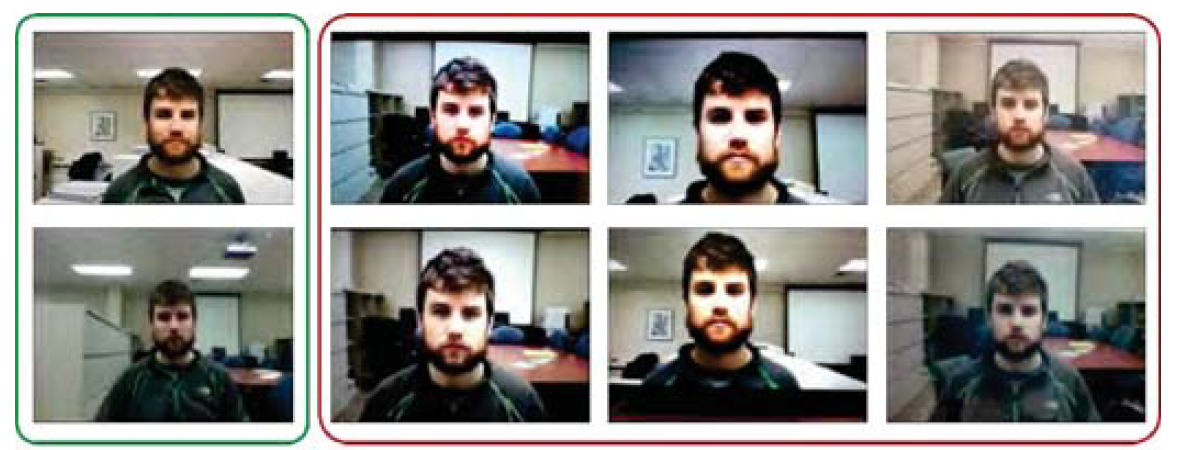
\includegraphics[width=\linewidth]{msu}}
	\caption{نمونه‌هایی از دیتاست MSU \cite{wen2015face} }
	\label{fig:msu}
\end{figure}

\subsection{دیتاست OULU}
در دیتاست OULU
\cite{boulkenafet2017oulu}
از 55 شخص مختلف برای تصویر برداری نمونه‌های واقعی و تقلبی استفاده شده است. تصویربرداری در سه نشست مختلف، با شش تلفن همراه جدید در زمان جمع‌آوری دیتاست استفاده شده است که باعث تنوع در کیفیت تصویر و محیط پس‌زمینه شده است. برای حمله کاغذ چاپ شده از دو نوع چاپگر با کیفیت و برای حمله بازپخش از یک نمایش‌گر و صفحه نمایش لپ‌تاپ استفاده است. ویدیوهای ضبط شده با کیفیت full HD با رزولوشن 1920*1080 گرفته شده است.

این دیتاست در مقایسه با دیتاست‌های قبلی تنوع بیشتر و کیفیت بالاتری دارد که باعث چالشی شدن دیتاست شده‌است. نمونه‌های واقعی در دیتاست OULU در شکل 
\ref{fig:oulureal}
 نشان داده شده است و نمونه‌های حمله در شکل 
 \ref{fig:oulufake}
 نشان داده شده است که دو نمونه‌ی سمت چپ دو نوع حمله کاغذ چاپ‌شده و نمونه‌های سمت راست دو نوع حمله باز پخش را نشان می‌دهد. 
 
  \begin{figure}[h]
 	\centerline{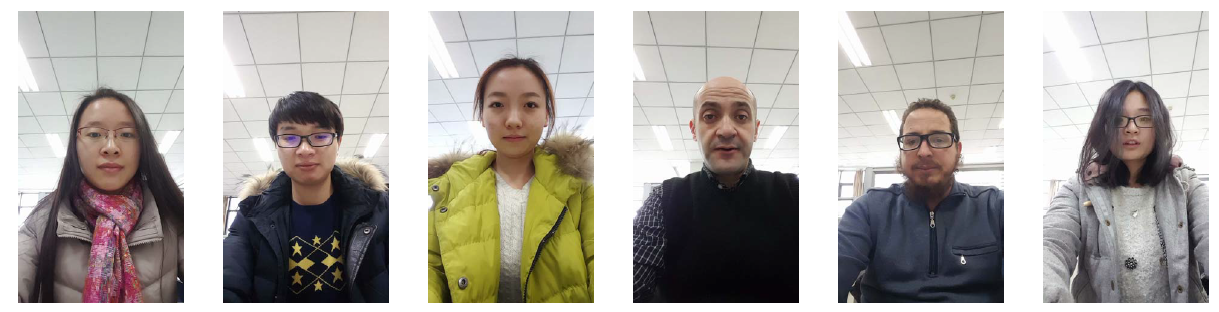
\includegraphics[width=\linewidth]{oulureal}}
 	\caption{نمونه‌های واقعی در دیتاست OULU \cite{boulkenafet2017oulu} }
 	\label{fig:oulureal}
 \end{figure}
 
 
  \begin{figure}[h]
 	\centerline{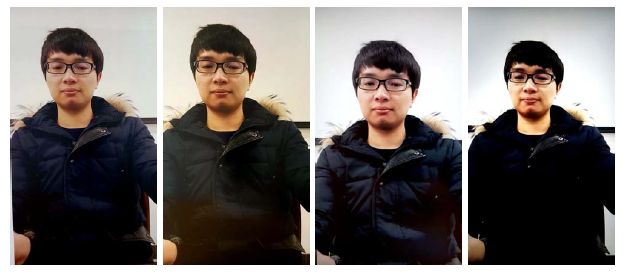
\includegraphics[width=\linewidth]{oulufake}}
 	\caption{نمونه‌های تقلبی در دیتاست OULU \cite{boulkenafet2017oulu} }
 	\label{fig:oulufake}
 \end{figure}
 
همچنین در این دیتاست برای گزارش دقت چهار پروتکل مختلف به‌منظور ارزیابی قابلیت تعمیم‌پذیری مدل ارائه شده در حالت‌های مختلف پیشنهاد شده‌است. پروتکل اول تنوع نشست را در دقت مدل بررسی می‌کند، بدین صورت که مدل باید روی داده‌های دو نشست از سه نشست آموزش ببیند و ارزیابی روی نشست سوم خواهد بود. در پروتکل دوم روی یک نوع از حمله کاغذ چاپ شده و یک نوع حمله‌ی بازپخش آموزش انجام می‌شود و در ارزیابی از نوع دیگر حمله باز پخش و کاغذ چاپ‌شده استفاده می‌شود تا تعمیم پذیری مدل روی حمله از ابزار دیده نشده بررسی شود. در پرتوکل سوم روی 5 نوع دوربین تلفن همراه از شش نوع آموزش انجام می‌شود و روی نوع ششم ارزیابی صورت می‌گیرد که این حالت برای بررسی قابلیت تعمیم پذیری روی نوع سنسور تصویر برداری دیده نشده انجام می‌گردد. پروتکل چهارم هر سه نوع پرتکل قبلی در هم ادغام می‌شوند تا اثر تنوع نشست، تنوع دوربین و تنوع نوع حمله ملاحظه شود.
\subsection{دیتاست SIW}
در دیتاست SIW
\cite{liu2018learning}
از 165 شخص مختلف برای تصویربرداری استفاده شده است. برای تصویربرداری از دو نوع دوربین با کیفیت استفاده شده است. در نمونه‌های واقعی تصویر برداری با فواصل مختلف دوربین تا کاربر انجام شده است تا تنوع فاصله کاربر با دوربین را پوشش دهد. همچنین از کاربر خواسته شده است که حالات مختلف چهره را به خود بگیرد و صورت خود را حرکت بدهد. این موجب تنوع در زاویه چهره نسب به دوربین و تنوع حالات چهره شده است. همچنین شرایط نورپردازی مختلف در این دیتاست دیده شده است. از دو نوع چاپگر برای حمله کاغذ چاپ‌شده استفاده شده‌است و از کاربر خواسته شده‌است که در دو حالت کاغذ را ثابت نگه دارد و آن را حرکت بدهد. همچنین از تبلت و دو نوع گوشی و صفحه نمایش‌گر رایانه برای حمله بازپخش استفاده شده است. نمونه‌های این دیتاست در  شکل 
\ref{fig:siw}
قابل مشاهده است. 
  \begin{figure}[h]
	\centerline{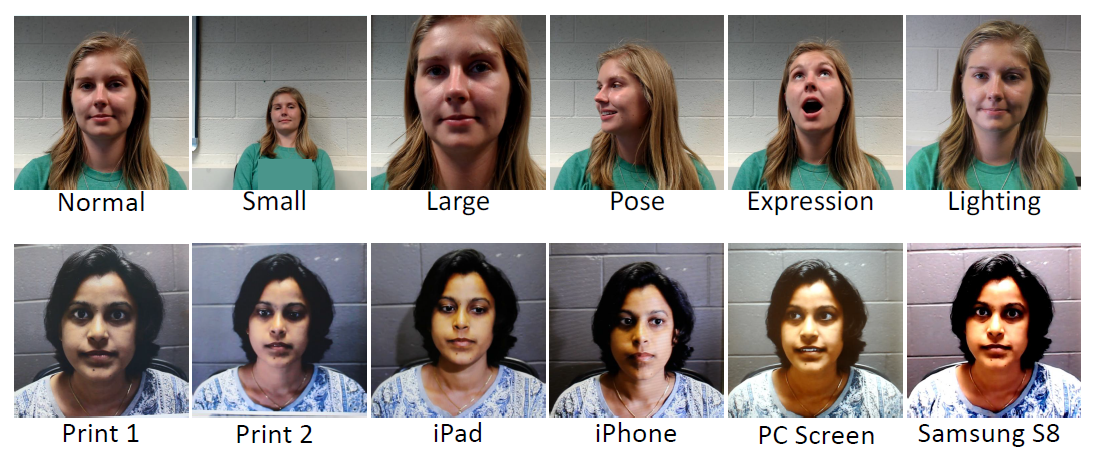
\includegraphics[width=\linewidth]{siw}}
	\caption{نمونه‌های از دیتاست SIW \cite{liu2018learning} }
	\label{fig:siw}
\end{figure}

این دیتاست دارای سه نوع پروتکل مختلف برای ارزیابی است. در پروتکل اول تنها از 60 فریم اول هر ویدئو برای آموزش استفاده می‌شود و از تمامی فریم‌های ویدیوهای تست برای ارزیابی استفاده می‌شود. از آنجا که در فریم‌های ابتدایی ویدئو کاربر صورت خود را حرکت نمی‌دهد این پروتکل به ارزیابی تغییر حالت چهره می‌پردازد. در پروتکل دوم از سه نوع حمله بازپخش استفاده می‌شود و روی حمله چهارم بازپخش ارزیابی می‌شود تا اثر تنوع ابزار حمله در بازپخش بررسی شود. در پروتکل سوم از یکی از انواع حمله بازپخش یا چاپ برای آموزش استفاده می‌شود و از نوع حمله دیگر برای تست استفاده می‌شود که هدف آن ارزیابی نوع حمله دیده نشده است. 





 











 












		% فصول دوم: مروری بر مطالعات انجام شده
% !TeX root=../main.tex

\chapter{روش پیشنهادی}
%\thispagestyle{empty} 
\section{مقدمه} 
در این فصل به توضیح مبانی نظری روش پیشنهادی پرداخته می‌شود. روش پیشنهادی شامل یک عملگر قابل آموزش با فرمول بندی شبیه \lr{LBP} و قرار دادن این عملگر در لایه اول شبکه کانولوشن کلاسیک است. از آنجا که در مسئله کشف تقلب به‌جای تمرکز روی ویژگی‌های ظاهری نظیر گوشه‌ها، لبه‌ها و... اطلاعات بافت تصاویر اهمیت دارد این لایه مبتنی بر \lr{LBP} پیشنهاد شده است. 
ابتدا عملگر \lr{LBP} قابل آموزش بیان خواهد شد. سپس ساختار شبکه تشریح خواهد شد و در ادامه به توضیح تابع هزینه معرفی شده پرداخته می‌شود. 

برای بیان عملگر \lr{LBP} قابل آموزش ابتدا توضیحی کلی از عملگر کانولوشن و شبکه‌های کانولوشنی همراه با شهود استفاده از این شبکه‌ها در مسائل بینایی ماشین، بیان خواهد شد. سپس رابطه ریاضی عملگر کانولوشن و عملگر \lr{LBP} ارائه شده و با همانندسازی این دو عملگر، عملگر \lr{LBP} قابل آموزش به‌دست خواهد آمد.
در ادامه برای بهینه کردن شبکه با هدف بهبود دقت و افزایش قابلیت تعمیم‌پذیری، دو تابع هزینه معرفی خواهد شد. در تابع هزینه اول هدف تفکیک کردن دو کلاس با حاشیه است و در تابع هزینه دوم هدف مجبور کردن شبکه به توجه به ویژگی‌های تقلب به‌جای توجه به ویژگی‌های ظاهری افراد است.
\section{مروری بر عملگر کانولوشن}
یکی از اجزای اصلی شبکه‌های مبتنی بر یادگیری عمیق عملگر کانولوشن است. این عملگر دارای یک هسته‌ی ضرایب است که به‌صورت پیچشی در تصویر ورودی ضرب می‌شود و سپس با لغزش بر کل تصویر ورودی، یک تصویر خروجی به‌دست خواهد آمد. 

اعمال عملگر کانولوشن روی سیگنال معادل ضرب تبدیل فوریه عملگر در تبدیل فوریه تصویر ورودی است و با این ضرب می‌توان برخی از فرکانس‌های تصویر ورودی را تقویت یا تضعیف کرد که فیلتر کردن تصویر ورودی خواهد بود. اعمال وزن‌های مختلف به هسته فیلتر می‌تواند خروجی تصویر با مشخصات خاصی را بدهد.

برای مثال با استفاده از وزن‌های خاص در عملگر می‌توان یک فیلتر پایین‌گذر طراحی کرد و با اعمال عملگر کانولوشن این فیلتر پایین‌گذر، یک تصویر که فرکانس‌های بالای آن حذف شده‌اند به‌دست آورد. طراحی فیلترهای مختلف برای اهداف گوناگونی نظیر یافتن لبه در تصویر یا حذف نویز تصویر می‌تواند کاربرد داشته باشد. اما هر هدف نیازمند یک فیلتر خاص از قبل طراحی شده است. 

ایده شبکه‌های عصبی کانولوشنی
\LTRfootnote{Convolutional neural network} (\lr{CNN}) 
در این است که وزن‌های فیلتر به‌صورت پارامتر در نظر گرفته شود و در طی فرآیند بهینه‌سازی تابع هزینه، ضرایب فیلتر به‌روزرسانی شوند و فیلترهای مد نظر از طریق داده‌های موجود به‌دست آیند. 
هر اعمال یک لایه کانولوشن روی تصویر باعث به‌دست آوردن ویژگی‌ها جدید می‌شود و با اعمال متوالی عملگر پارامتری شده کانولوشن، ویژگی‌های مفهومی‌تر به‌دست خواهد آمد. این ساختار لایه‌ای در صورتی که با تعداد کافی داده، بهینه شود می‌تواند ویژگی‌های معنایی از تصویر را استخراج کند. که این دریافت معنا از تصویر باعث کاربردهای مختلفی نظیر طبقه‌بندی، تشخیص شئ، شناسایی چهره و... شده است.

در مسئله تشخیص تقلب در تشخیص چهره، بیش از آنکه ویژگی‌های معنایی تصویر مد نظر باشد یافتن ویژگی‌هایی در تصویر که شاخصی برای واقعی یا تقلبی بودن چهره است اهمیت دارد. در واقع هدف این است که شبکه‌ای طراحی شود که نشانه‌های تقلب در تصویر را پیدا کند. یکی از ویژگی‌های نشانه‌های تقلب در تصویر وجود در مقیاس ریز تصویر است به‌گونه‌ای که در نگاه اول تشخیص آن دشوار به نظر می‌آید. یکی دیگر از ویژگی‌های نشانه‌ی تقلب در تصویر وجود آن در بیشتر بخش‌های چهره است. بدین منظور در گام اول عملگری ارائه شده است که هدف آن تحلیل بافت تصویر و کمک گرفتن از ایده‌ی شبکه عصبی به‌منظور یافتن بهترین عملگر با توجه به داده‌های ورودی شبکه است.

\section{عملگر \lr{LBP} قابل آموزش}
در این بخش فرمول بندی عملگر 
\lr{LBP}
قابل آموزش بیان می‌شود. بدین منظور ابتدا رابطه عملگر کانولوشن بیان شده و سپس رابطه ریاضی 
\lr{LBP}
کلاسیک بیان خواهد شد. سپس با مقایسه رابطه کانولوشن و رابطه 
\lr{LBP}
کلاسیک، این رابطه به نحوی تغییر داده می‌شود که همانند کانولوشن دارای پارامتر  قابل یادگیری باشد اما بر خلاف کانولوشن به جای فیلتر کردن تصویر یک خروجی متناظر با بافت تصویر مطابق فرمول 
\lr{LBP}
به صورت پارامتری شده بدهد.

رابطه عملگر کانولوشن و تصویر ورودی به‌صورت رابطه 
\ref{eq:cnn}
است. که در آن 
$I_p$
مقدار شدت روشنایی تصویر در پیکسل $p$ در یک همسایگی یا پنچره به ابعاد فیلتر است. و 
 $W_p$
مقدار وزن متناظر فیلتر در مختصات $p$ پنجره عملگر است. و تابع
$\sigma(.)$  
نیز یک تابع غیر خطی است.

\begin{equation}\label{eq:cnn}
	CNN=\sigma(\sum_{p\in N}I_pW_p)
\end{equation}
و همچین رابطه عملگر ریزبافت
\lr{LBP}
 به‌صورت رابطه
\ref{eq:lbp}
 است.که در آن
$I_c$
   مقدار روشنایی پیکسل در مرکز پنجره عملگر است. در واقع در این عملگر در یک همسایگی، مقدار هر پیکسل از پیکسل مرکزی کسر می‌گردد و بر اساس خروجی بزرگ‌تر یا کوچک‌تر بودن از صفر، یک وزن  
$2^p$   
   پیدا می‌کند. این وزن به‌صورت ایستا و طبق تعریف قراردادی عملگر مشخص می‌گردد.
\begin{equation}\label{eq:lbp}
	LBP=\sum_{p\in N}\sigma(I_p-I_c)2^p 
\end{equation}

	\[ \sigma(x) = 
	\begin{cases} 1  & \text{$x \geq 0 $}\,; \\
		0  & \text{\lr{otherwise}}\,.
	\end{cases} \]


به‌منظور آن‌که از ایده یافتن وزن‌های بهینه از طریق داده در این عملگر استفاده شود لازم است که تعریف این عملگر به‌جای تعریف ایستان به تعریف پارامتری شده برسد. بدین منظور وزن
$2^p$
 به‌صورت رابطه
\ref{eq:expon}
 تغییر داده می‌شود.
\begin{equation}\label{eq:expon}
	2^p=e^{p\ln{2}}=e^{w_p}
\end{equation}

که در آن 
$W_p$
 یک پارامتر است که حین بهینه‌سازی تغییر می‌کند تا به بهترین مقدار مناسب برای طبقه‌بندی برسد. با جایگذاری این پارامتر در رابطه \lr{LBP} کلاسیک، عملگر \lr{LBP} قابل آموزش به‌دست خواهد آمد به‌صورت رابطه
\ref{eq:lbptr}
به‌دست خواهد آمد.
\begin{equation}\label{eq:lbptr}
		LBP_{tr}=\sum_{p\in N}\sigma(I_p-I_c)e^{W_p} 
\end{equation}

این عملگر در مقایسه با عملگر کانولوشن نگاه ریزتری به بافت تصویر خواهد داشت. از آن‌جا که در کانولوشن تمامی پیکسل‌های همسایگی در وزن‌های فیلتر ضرب شده و حاصل جمع آنها در تابع غیر خطی قرار می‌گیرند، در عملگر کانولوشن تمامی پیکسل‌های همسایگی تأثیری به‌اندازه وزن متناظر خود در خروجی دارند. اما در عملگر \lr{LBP} از آن‌جا که تابع غیر خطی بین تفاضل هر پیکسل با پیکسل مرکزی اعمال می‌شود نگاه جزئی‌تری به تصویر خواهد داشت و باعث استخراج ویژگی‌های بافتی تصویر خواهد شد. 

تابع 
$\sigma(.)$
 یک تابع غیر خطی است که نقشی مشابه تابع فعالسازی
\LTRfootnote{Activation function}
  در شبکه‌های عصبی را بازی می‌کند. وظیفه این تابع ایجاد روابط غیرخطی برای عملگر است و تفاوت مهم عملگر \lr{LBP} قابل آموزش با کانولوشن در اعمال تابع غیرخطی درون عملگر مجموع‌گیری است در حالی که در کانولوشن‌های شبکه عصبی تابع غیر خطی بیرون عملگر  مجموع‌گیری قرار دارد. هر چند که تعریف کلاسیک برای عملگر \lr{LBP} استفاده از تابع \lr{Heaviside} است اما از توابع غیر خطی دیگری نظیر \lr{Relu} و \lr{Sign} نیز می‌توان استفاده کرد.
  
لازم به ذکر است که نحوه بهینه‌سازی شبکه‌های عصبی که دارای لایه‌های متوالی هستند با استفاده از مشتق‌گیری از تابع هزینه که در انتهای شبکه‌ی عصبی قرار دارد با الگوریتم پس انتشار
\LTRfootnote{Back propagation}
 است. برای آن‌که روال بهینه‌سازی به درستی کار کند لازم است که هر کدام از عملگرهای شبکه عصبی مشتق پذیر باشد. برای بررسی مشتق‌پذیری عملگر پیشنهادی، مشتق این عملگر نسبت به یکی از پارامتر‌های آن یعنی 
$W_{p^*}$
طبق رابطه
\ref{eq:lbptrdif}
بررسی می‌گردد.
 
\begin{align}\label{eq:lbptrdif}
	\frac{\partial LBP_{tr}}{\partial W_{p^*}} 
	&= \frac{\partial (\sum_{p\in N}\sigma(I_p-I_c)e^{W_p}) }{\partial W_{p^*}} 
	= \sum_{p\in N} {\frac{\partial (\sigma(I_p-I_c)e^{W_p}) }{\partial W_{p^*}} }
	\\&= 	\frac{\partial (\sigma(I_{p^*}-I_c)e^{W_{p^*}})}{\partial W_{p^*}}
	= \sigma(I_{p^*}-I_c)e^{W_{p^*}}
	\nonumber
	%LBP_{tr}=\sum_{p\in N}\sigma(I_p-I_c)e^{W_p} 
\end{align}
همانطور که مشاهده می‌شود مشتق عملگر پیشنهادی دارای یک مقدار 
$e^{W_{p^*}}$
درون خود است. برای آنکه فرآیند بهینه‌سازی هموارتر شود می‌توان تعریف عملگر پیشنهادی در رابطه 
\ref{eq:lbptr}
به جای مقدار 
$e^{W_p}$
مقدار 
$W_p$
جایگزین شود در این صورت رابطه عملگر قابل آموزش به صورت رابطه 
\ref{eq:lbptrlin}
خواهد شد و مشتق آن نیز به صورت رابطه 
\ref{eq:lbptrlindif}
خواهد بود.
\begin{equation}\label{eq:lbptrlin}
	LBP_{tr}=\sum_{p\in N}\sigma(I_p-I_c)W_p 
\end{equation}

\begin{equation}\label{eq:lbptrlindif}
	\frac{\partial LBP_{tr}}{\partial W_{p^*}}=
	\sigma(I_{p^*}-I_c)
\end{equation}


\begin{figure}[ht]
	\centerline{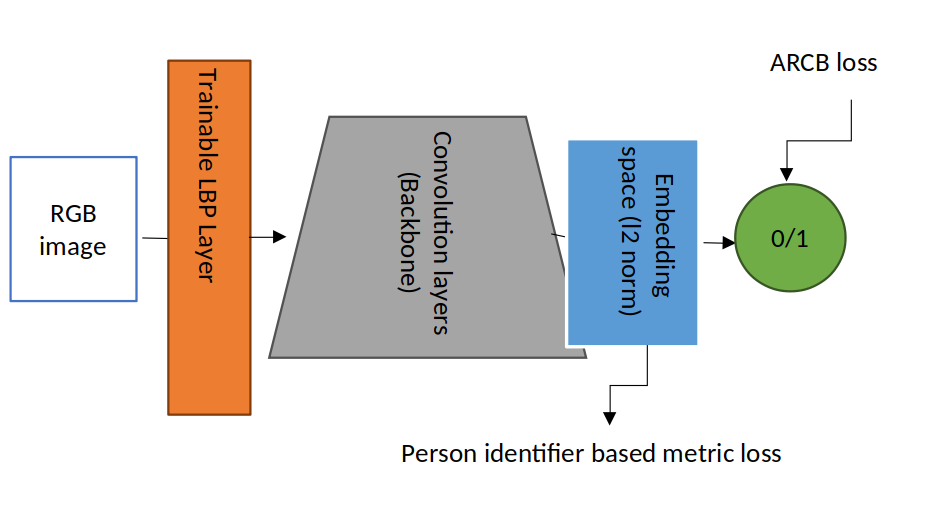
\includegraphics[width=\linewidth]{model}}
	\caption{شمای کلی روش پیشنهادی}
	\label{fig:model}
\end{figure}  
\section{ساختار شبکه}
 از آنجا که عملگر  
$LBP_{tr}$
 یک عملگر تحلیل تصویر در مقیاس ریز است، از این عملگر به‌عنوان لایه اول شبکه عمیق استفاده می‌شود. پس ساختار شبکه به‌صورت شکل 
\ref{fig:model}
 خواهد بود.
 تصویر ورودی به‌صورت سه کانال رنگی وارد عملگر   می‌شود و خروجی آن به یک شبکه متشکل از لایه‌های کانولوشن داده می‌شود که در این پژوهش از شبکه
  \lr{EfficientNet B0} \cite{tan2019efficientnet}
 استفاده شده است. شبکه 
 \lr{EfficientNet}
 دارای هفت نسخه شبیه به هم اما با ابعاد مختلف است که طی یک الگوریتم جست‌و‌جوی معماری شبکه به‌دست آمده است. در این پژوهش از نسخه پایه‌ی آن استفاده می‌شود. نسخه‌های بعدی آن ابعاد بزرگ‌تری دارند که این ابعاد از طریق بهینه سازی به دست آمده است و دقت بهتری نیز ارائه می‌کنند.
 
 جزئیات ساختار ارائه شده در جدول 
 \ref{tab:network}
 گزارش شده است. در لایه‌ی اول از عملگر معرفی شده استفاده می‌شود. در لایه‌های بعدی از بلوک‌های
 \lr{MBConv}
 استفاده شده است که بلوک‌های پایه شبکه 
 \lr{Mobilenetv2} \cite{sandler2018mobilenetv2}
 است با این تفاوت که 
 \lr{squeeze and excitation} \cite{hu2018squeeze}
 نیز به آن اضافه شده است.
 
 پس از اعمال لایه‌های کانولوشنی یک بردار مسطح با بعد 1280 خواهد بود که با توجه به تابع هزینه‌های مورد استفاده این خروجی لازم است نرمالایز شود.این خروجی نرمالایز شده با یک لایه خطی دیگر به یک نورون ختم خواهد شد. تک نورون لایه‌ی آخر مقداری بین صفر و یک خواهد داشت که برحسب مقدار این نورون و انتخاب یک سطح آستانه طبقه‌بندی دو کلاسه صورت خواهد گرفت.
 
  خروجی نرمالایز شده شبکه کانولوشنی در دو تابع هزینه به کار برده می‌شود. تابع هزینه اول که ‌
 \lr{ARCB}
 نام دارد برای طبقه‌بندی با حاشیه در فضای کسینوسی پیشنهاد شده است که با توجه به فرمول‌بندی آن، لازم است که بردار ویژگی نرمالایز باشد. در تابع هزینه دوم که مبتنی بر شناسه اشخاص است از فاصله اقلیدسی بردار‌های ویژگی نرمالایز شده استفاده می‌کند.
 \begin{table}[h]
 	\caption{ساختار شبکه پیشنهادی}
	\label{tab:network}
	\centering
	\onehalfspacing
	
	\begin{tabular}{|c|c|c|c|}
		\hline
		\lr{Stage} & \lr{Operator} & \lr{Resolution} & \lr{\#Channels} \\ \hline
		\lr{0} & \lr{ُTainable LBP} & \lr{224 × 224} & \lr{3} \\ \hline
		\lr{1} & \lr{Conv3x3} & \lr{224 × 224} & \lr{32} \\ \hline
		\lr{2} & \lr{MBConv1, k3x3} & \lr{112 × 112} & \lr{16} \\ \hline
		\lr{3} & \lr{MBConv6, k3x3} & \lr{112 × 112} & \lr{24} \\ \hline
		\lr{4} & \lr{MBConv6, k5x5} & \lr{56 × 56}  & \lr{40} \\ \hline
		\lr{5} & \lr{MBConv6, k3x3} & \lr{28 × 28} & \lr{80} \\ \hline
		\lr{6} & \lr{MBConv6, k5x5} & \lr{14 × 14} & \lr{112} \\ \hline
		\lr{7} & \lr{MBConv6, k5x5} & \lr{14 × 14} & \lr{192} \\ \hline
		\lr{8} & \lr{MBConv6, k3x3} & \lr{7 × 7} & \lr{320} \\ \hline
		\lr{9} &\lr{Conv1x1 \& Pooling}  & \lr{7 × 7} & \lr{1280} \\ \hline
		\lr{10} & \lr{Normalization \& Linear} & \lr{1280} & \lr{1} \\ \hline
	\end{tabular}
\end{table}
 
 تابع هزینه متداول در شبکه عصبی برای طبقه‌بندی دو کلاسه تابع آنتروپی متقاطع دودویی
\LTRfootnote{Binary cross entropy} 
   (\lr{BCE}) است. اما تحقیقات پیشین در حوزه کشف تقلب نشان داده است که این تابع 
   هزینه به تنهایی مؤثر واقع نخواهد شد. به همین منظور تابع هزینه جدیدی برای طبقه‌بندی معرفی می‌گردد که یک حاشیه امن برای طبقه بندی ایجاد کند که باعث افزایش قابلیت تعمیم‌پذیری شبکه خواهد شد.
\section{تابع هزینه \lr{ARCB}}
در شبکه‌های عصبی زمانی که خروجی یک طبقه‌بندی چند کلاسه (بیشتر از دو) باشد از تابع فعالسازی سافتمکس
\LTRfootnote{SoftMax}
 در لایه‌ی آخر استفاده می‌شود و در طبقه بندی دو کلاسه از تابع فعالسازی سیگموید 
\LTRfootnote{Sigmoid} 
 استفاده می‌شود. دنگ و همکاران در حوزه تشخیص چهره
 \LTRfootnote{Face recognition}
  که یک طبقه‌بندی چند کلاسه است تابع هزینه آنتروپی متقاطع
 \LTRfootnote{Cross entropy}
   (\lr{CE}) را به فضای کسینوسی برده‌اند و یک حاشیه به تابع هزینه در این فضا اضافه کرده‌اند
\cite{deng2019arcface}.

با الهام از این کار که \lr{ArcFace} نام‌گذاری شده است در این پایان‌نامه، تابع هزینه \lr{BCE} با هدف اعمال حاشیه در فضای کسینوسی بازنویسی می‌شود. فرض کنید خروجی شبکه استخراج ویژگی یک بردار  باشد. در تصمیم‌گیری کلاسیک این بردار با بعد $d$ وارد یک لایه شبکه عصبی با ورودی $d$ نورون و خروجی یک نورون خواهد شد. و نهایتاً از تابع سیگموید برای بردن مقدار خروجی به مقدار بین یک و صفر استفاده خواهد شد.
در تصمیم‌گیری دو کلاسه رابطه تابع هزینه آنتروپی متقاطع دودویی به‌صورت رابطه
\ref{eq:bce}
است.
\begin{equation}\label{eq:bce}
	L_{BCE} = -y_i \log{P(y_i)} - (1-y_i)\log{( 1-P(y_i) )}
\end{equation}

 که در آن 
$y_i$
  برچسب صحیح متناظر با بردار ویژگی   است. و 
$P(y_i)$
   مقدار نورون لایه آخر است، در واقع این مقدار از نوع احتمال است یعنی مقداری بین صفر و یک دارد و هر چه به یک نزدیک‌تر باشد می‌توان با احتمال بیشتری تصمیم‌گیری کرد که خروجی طبقه‌بندی عدد یک است.
رابطه بین نورون خروجی و بردار ویژگی   به‌صورت رابطه
\ref{eq:pyi}
است.
\begin{equation}\label{eq:pyi}
	P(y_i) = sigmoid(W^TX_i+b)
\end{equation}

که در آن  
$W_p \in R^d$
وزن لایه‌ی آخر و $b$ مقدار بایاس است. برای سادگی فرض می‌شود که بایاس صفر است.  تابع سیگموید به‌صورت رابطه
$sigmoid(x) = \frac{1}{1+e^{-x}}$
 تعریف می‌شود.پیش از لایه آخر شبکه عصبی مقدار وزن‌های 
$W_p$
 نرمالایز کرده بردار ویژگی 
 $X_i$
  را نرمالایز کرده و سپس مقیاس $s$ به آن داده می‌شود. این مقیاس‌گذاری برای پایدار کردن فرآیند بهینه سازی صورت گرفته است.
  با نرمالایز کردن مقدار ضرب داخلی بین وزن و بردار ویژگی معادل کسینوس زاویه بین این دو بردار خواهد شد.
 \begin{equation}\label{eq:wti}
	W^TX_i = |W^T||X_i| \cos{\theta_i}=s\cos{\theta_i}
 \end{equation}
حال با جاگذاری این مقدار در تابع هزینه \lr{BCE} به‌صورت رابطه
\ref{eq:bcenorm}
 بازنویسی می‌شود.
\begin{equation}\label{eq:bcenorm}
	L_{BCE} = -y_i \log{\frac{1}{1+e^{-s\cos{\theta_i}}}} - (1-y_i)\log{(1-\frac{1}{1+e^{-s\cos{\theta_i}}} )}
\end{equation}

با توجه به مقداری برچسب واقعی  که صفر یا یک است دو حالت رخ می‌دهد.

حالت اول. زمانی که برچسب یک باشد در این صورت تنها عبارت اول در رابطه 
\ref{eq:bcenorm}
 ظاهر می‌شود. در این حالت مطلوب این است که مقدار داخل لگاریتم بیشینه شود که این معادل این است که زاویه بین بردار ویژگی و وزن لایه آخر به صفر نزدیک شود. برای آنکه بهینه‌سازی با یک حاشیه انجام شود یک مقدار حاشیه $m$ را به آن افزوده می‌شود.
  \begin{equation}\label{eq:st1}
 	y_i=1 \to \theta_i= \theta_i + m
 \end{equation}

حالت دوم. زمانی که مقدار برچسب واقعی صفر باشد در این صورت عبارت دوم در رابطه 
\ref{eq:bcenorm}
 ظاهر می‌گردد. بدین منظور لازم است که عبارت داخل لگاریتم کمینه شود که معادل این است که زاویه بین وزن و بردار ویژگی به مقدار 
$\pi$
  نزدیک شود. برای آنکه بهینه‌سازی با حاشیه انجام شود یک مقدار ثابت حاشیه $m$ از زاویه بین دو بردار کم می‌شود.
   \begin{equation}\label{eq:st2}
 	y_i=0 \to \theta_i= \theta_i - m
 \end{equation}

با جایگذاری زاویه‌های حاشیه دار شده در روابط 
\ref{eq:st1}
 و 
 \ref{eq:st2}
 در رابطه تابع هزینه \lr{BCE} بازنویسی شده در فضای کسینوسی 
 \ref{eq:bcenorm}
 تابع هزینه \lr{ARCB} به‌صورت رابطه
\ref{eq:arcb}
  به‌دست خواهد آمد.
\begin{equation}\label{eq:arcb}
	L_{BCE} = -y_i \log{\frac{1}{1+e^{-s\cos{(\theta_i+m)}}}} - (1-y_i)\log{(1-\frac{1}{1+e^{-s\cos{(\theta_i-m)}}} )}
\end{equation}

این تابع هزینه نه تنها ویژگی‌های بین دو کلاس را جدا می‌کند بلکه یک حاشیه به‌اندازه  
$2*m$
نیز به ویژگی‌های دو کلاس مختلف در فضای کسینوسی اضافه می‌کند. این حاشیه باعث می‌شود که در فرآیند بهینه‌سازی، وزن‌های شبکه به‌گونه‌ای تغییر کنند که قابلیت تعمیم‌پذیری شبکه بیشتر شود.
در شکل
\ref{fig:arcb}
تفاوت بین تابع هزینه کلاسیک و تابع هزینه با حاشیه نشان داده شده است. در صورتی که تابع هزینه به‌درستی بهینه شود باعث می‌شود که در لایه آخر بردارهای ویژگی در فضای کسینوسی به نحوی قرار بگیرند که زاویه بین نمونه‌ی جدید با بردار وزن در حالتی که برچسب یک است به سمت صفر میل کند و در حالتی که برچسب صفر است زاویه به سمت  میل کند. و همچنین اثر افزودن حاشیه در تقسیم پذیری بین دو کلاس قابل مشاهده است. در شکل
\ref{fig:arcb}
در سمت چپ نتیجه جداسازی بردارهای ویژگی در حالت استفاده از تابع هزینه \lr{BCE} را نشان می‌دهد و در سمت راست تابع هزینه \lr{ARCB} باعث جدا شدن بردارهای ویژگی با یک حاشیه در فضای کسینوسی شده است. 
\begin{figure}[h]
	\centerline{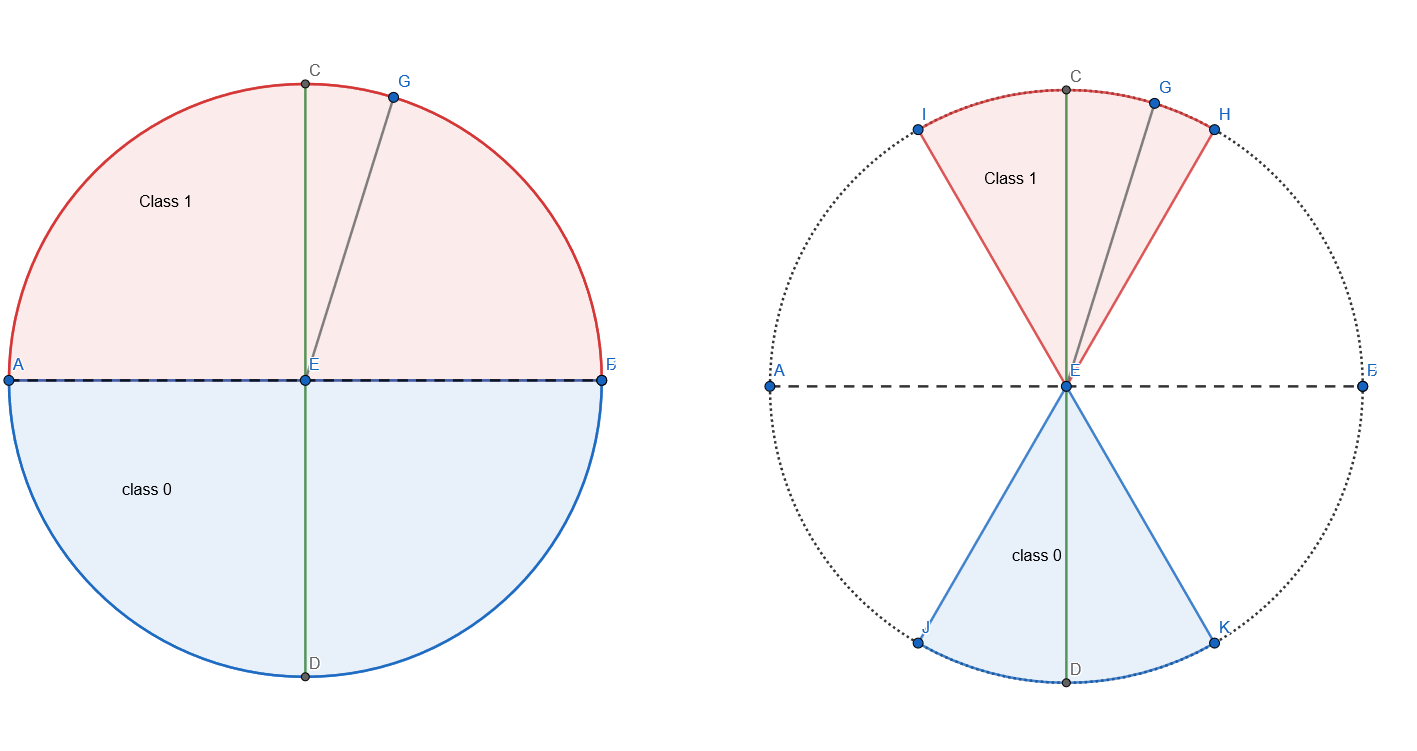
\includegraphics[width=0.8\linewidth]{arcb}}
	\caption{مقایسه تابع هزینه
		 \lr{BCE} 
		کلاسیک با نسخه‌ی حاشیه‌دار
	\lr{ARCB} }
	\label{fig:arcb}
\end{figure}

\section{تابع هزینه بر اساس شناسه‌ی شخص}
در دیتاست‌های موجود در حوزه کشف تقلب در چهره، برای هر فرد چند نمونه‌ی زنده و چند نمونه تقلبی وجود دارد. یعنی یک فرد که از چهره او برای جمع‌آوری داده استفاده شده است نمونه فیلم زنده و تقلبی او ضبط شده است. در ویدیو واقعی و تقلبی فرد در دیتاست یک ویژگی ظاهری یکسان شامل مشخصه‌های چهره‌ی وی وجود دارد که این مشخصه‌ها با فرد دیگر متفاوت است. از طرفی در فرآیند آموزش شبکه مطلوب این است که شبکه به‌جای تمرکز روی ویژگی‌های ظاهری چهره‌ی افراد روی علائم مربوط به وجود یا عدم وجود تقلب در چهره تأکید داشته باشد.

از آنجا که عمده تصویر ورودی به شبکه شامل چهره و مشخصات چهره می‌شود شبکه برای نمونه‌های مختلف از یک فرد دچار چسبندگی به روی ویژگی‌های چهره او خواهد شد که این امر مطلوب نیست.       
بدین جهت در این بخش یک جریمه برای این مورد در تابع هزینه قرار داده می‌شود که هدف شبکه این باشد که به ویژگی‌های ظاهری افراد توجه نکند و توجه آن به ویژگی‌های مربوط به تقلب باشد. فرض کنید بردار ویژگی خروجی قسمت استخراج ویژگی برای فرد $k$ ام با برچسب $l$ به‌صورت 
$X_k^l \in R^d , I \in \{0,1\}, K \in \{1,2,...,M\}$
 باشد.
در حین آموزش در هر گام تعداد دسته
\LTRfootnote{Batch size} $N$ 
فرض می‌شود. در میان این $N$ بردار ویژگی تعداد 
${N\choose 2}$
  جفت بردار ویژگی وجود دارد که در میان این تعداد جفت دو حالت مهم است.
  
  حالت اول زمانی که دو بردار ویژگی در جفت، متعلق به یک فرد ولی دارای برچسب مختلف هستند. یعنی 
  $k_1=k_2 , l_1 \ne l_2 $
  . در این حالت با توجه به اینکه مشخصه‌های ظاهری فرد که عمده تصویر ورودی است یکسان است لازم است که فاصله این دو نمونه بیشینه شود. با بیشینه کردن این فاصله شبکه مجبور می‌شود توجه خود را به‌جای مشخصه‌های ظاهری افراد به سمت ویژگی‌ای که تفاوت این دو نمونه است ببرد و این یعنی تفاوت برچسب این دو بردار ویژگی که یکی واقعی و یکی تقلبی است. 
  
  این حالت در شکل
\ref{fig:pid1}
  نشان داده شده است. در این شکل تصویر بالایی یک تصویر زنده و تصویر دومی تقلبی است. از آنجا که این دو تصویر شبیه هستند لذا خروجی بردارهای ویژگی آنها ممکن است که نزدیک هم باشند. بردارهای ویژگی به‌صورت ستاره در فضای $d$ بعدی نشان داده شده‌اند. لازم است که این فاصله بیشینه شود.
  
 \begin{figure}[ht]
 	\centerline{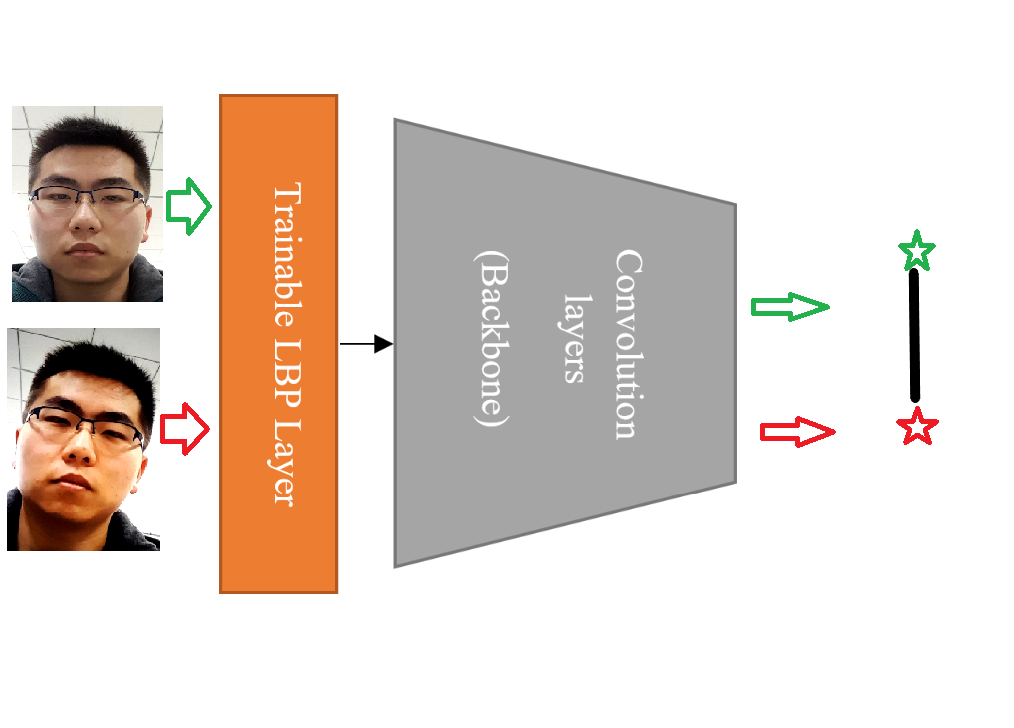
\includegraphics[width=\linewidth]{pid1}}
 	\caption{حالتی که دو نمونه متعلق به یک شخص ولی یکی واقعی و دیگری تقلبی است}
 	\label{fig:pid1}
 \end{figure}

پس در حالت اول هدف شبکه به‌صورت رابطه
\ref{eq:pid1obj}
است.
\begin{equation}\label{eq:pid1obj}
	\max_{\Theta} {d( X_{k_1}^{l_1},X_{k_2}^{l_2} )} = \min_{\Theta}{\max(0,M-d( X_{k_1}^{l_1},X_{k_2}^{l_2} ))}
\end{equation}

که در آن 
$\Theta$
 مجموعه وزن‌های شبکه را نشان می‌دهد و تابع $d$ فاصله اقلیدسی بین دو بردار ویژگی نرمالایز شده است و به‌صورت رابطه 
\ref{eq:dfunc}
  تعریف می‌شود.
  \begin{equation}\label{eq:dfunc}
  	d(X_1,X_2) = ||\frac{X_1}{||X_1||}-\frac{X_2}{||X_2||}||
  \end{equation}

از آنجا که باید در بهینه‌سازی تابع هزینه کمینه شود بیشینه‌سازی فاصله دو بردار ویژگی معادل کمینه سازی مقدار 
$\max(0,M-d( X_{k_1}^{l_1},X_{k_2}^{l_2} ))$
 خواهد بود. در این رابطه $M$ یک هایپر پارامتر است که در صورتی که فاصله دو بردار ویژگی از این مقدار بیشتر باشد مقدار خروجی صفر خواهد بود و در صورتی که کمتر باشد میزان فاصله تا این مقدار $M$ به عنوان مقدار هزینه خواهد بود.
با توجه به نامساوی رابطه
\ref{eq:ne}
بیشترین فاصله‌ای که دو بردار ویژگی در فضای نرمالایز شده خواهند داشت عدد 2 خواهد بود و در پیاده سازی این تابع هزینه مقدار $M$ عدد 2 در نظر گرفته شده است.
  \begin{equation}\label{eq:ne}
	||\frac{X_1}{||X_1||}-\frac{X_2}{||X_2||}|| \le ||\frac{X_1}{||X_1||}||+||\frac{X_2}{||X_2||}||   \to d(X_1,X_2) \le 2
\end{equation}

حالت دوم زمانی که دو بردار ویژگی در جفت دارای یک برچسب ولی متعلق به اشخاص مختلفی هستند. به بیان ریاضی یعنی  
  $k_1 \ne k_2 , l_1 = l_2 $
. در این حالت با توجه به تفاوت مشخصه‌های ظاهری اشخاص این دو بردار ویژگی ممکن است فاصله محسوسی در فضای ویژگی داشته باشند. در این حالت مطلوب این است که فاصله این دو بردار ویژگی کم شود. در این صورت شبکه مجبور خواهد شد که به‌گونه‌ای از تصویر ویژگی انتخاب کند که فاصله این دو بردار ویژگی کم باشد و با رسیدن به این هدف ویژگی‌های استخراج شده بیشتر روی ویژگی‌های کشف تقلب تا ویژگی‌های ظاهری افراد تأکید دارند.

در شکل
\ref{fig:pid2}
این حالت نشان داده شده است. در این مثال دو تصویر ورودی هر دو از نوع تقلبی هستند ولی متعلق به اشخاص مختلفی هستند. در این شکل ستاره نشان‌گر موقعیت بردار ویژگی متناظر با این دو ورودی در فضای
 $d$ 
بعدی است. از آنجا که دو فرد ویژگی‌های ظاهری متفاوتی دارند ممکن است فاصله بردارهای ویژگی متناظر با آن‌ها فاصله محسوسی داشته باشد. در این حالت کم کردن این فاصله مد نظر است. 
 \begin{figure}[ht]
	\centerline{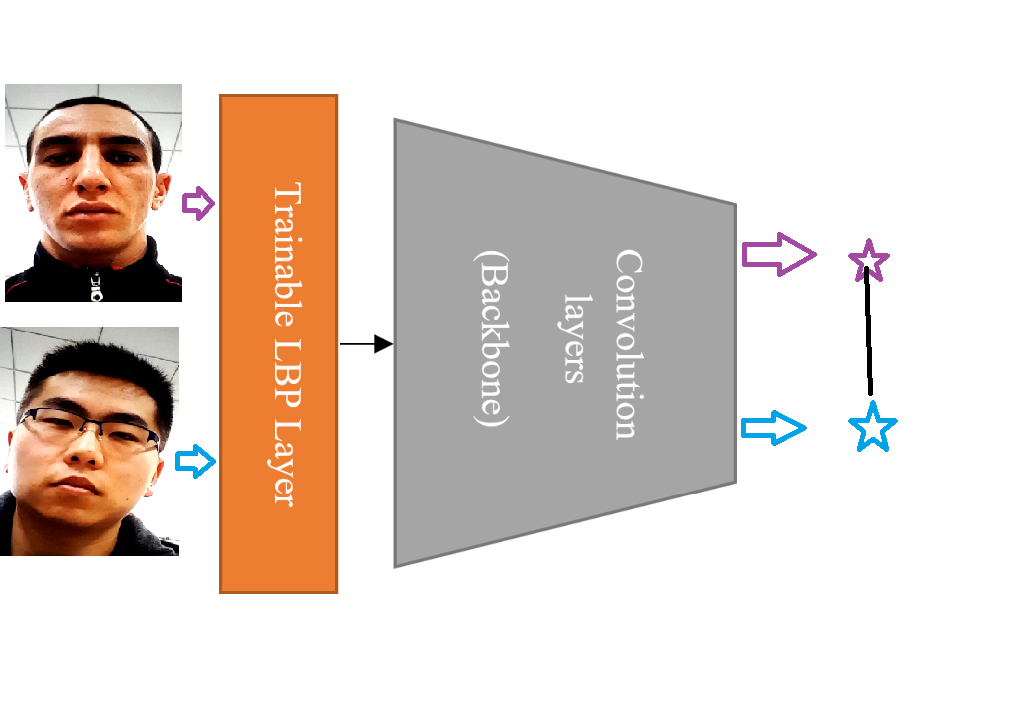
\includegraphics[width=\linewidth]{pid2}}
	\caption{حالتی که دو نمونه متعلق به اشخاص مختلف ولی برچسب یکسان هستند}
	\label{fig:pid2}
\end{figure}
پس به بیان ریاضی در این حالت تابع هزینه به‌صورت رابطه
\ref{eq:pid2obj}
خواهد بود.
\begin{equation}\label{eq:pid2obj}
\min_{\Theta} {d( X_{k_1}^{l_1},X_{k_2}^{l_2} )} 
\end{equation}

  و در نهایت تابع هزینه بر اساس شناسه اشخاص موجود در دیتاست به‌صورت رابطه
\ref{eq:pid}
  خواهد بود. که در آن  
 $N_i$
   تعداد جفت نمونه‌ها با ویژگی برچسب یکسان و شخص متفاوت در دسته است و 
   $N_j$
       تعداد جفت نمونه با ویژگی برچسب متفاوت و شناسه یکسان است.
\begin{equation}\label{eq:pid}
  	L_{PiD} = \sum_{l_1 \ne l_2,k_1 \ne k_2}{\frac{1}{N_i}d( X_{k_1}^{l},X_{k_2}^{l})+\frac{1}{N_j}\max(0,M-d( X_{k}^{l_1},X_{k}^{l_2} ))}
\end{equation}

 نحوه تشکیل این تابع هزینه بدین صورت است که در هر گام آموزش از میان $N$ نمونه‌ی موجود در دسته تمامی جفت‌هایی که شرط شناسه متفاوت برچسب یکسان و یا شرط شناسه یکسان و برچسب متفاوت دارند انتخاب شده و فاصله اقلیدسی آن‌ها در رابطه
\ref{eq:pid}
 قرار داده می‌شود. این تابع هزینه وقتی کمینه شود شبکه به سمتی حرکت می‌کند که ویژگی‌های مطلوب برای کشف تقلب شناسایی شده و ویژگی‌هایی مرتبط به چهره افراد نادیده گرفته شود.
 
 تابع هزینه معرفی شده در این قسمت بر خلاف تابع هزینه
 \lr{ARCB}
 وظیفه‌ی طبقه‌بندی ندارد و تنها به عنوان یک نقش کمکی در کنار طبقه‌بندی کمک می‌کند. لذا هرچند که تابع هزینه 
  \lr{ARCB}
  به تنهایی قابل استفاده است اما تابع هزینه مبتنی بر شناسه‌ی اشخاص به تنهایی قابل استفاده نیست. این تابع یک تابع هزینه متریک است که با استفاده از شناسه اشخاص محدودیت خاصی روی فاصله‌ی جفت نمونه‌های خاص ارائه می‌کند. تابع هزینه متریک به صورت غیر مستقیم باعث افزایش دقت طبفه‌بندی و بهبود قابلیت تعمیم‌پذیری شبکه خواهد شد. در واقع این تابع هزینه باعث می‌شود که شبکه‌ی استخراج ویژگی به نحوی عمل کند که بردار‌های ویژگی به نحو مناسبی قرار بگیرند که دقت طبقه‌بندی بیشتر شود و شبکه ویژگی‌های اساسی برای تقلب را فارغ از ویژگی‌های ظاهری افراد استخراج کند. لازم به ذکر است که ایده استفاده از تابع هزینه متریک در کنار طبقه‌بندی روشی کارآمد است که در حوزه کشف تقلب در چهره نیز با فرمول‌بندی‌های مختلف استفاده شده است
\cite{shao2019multi,jia2020single,feng2020learning,perez2019deep,tu2020learning,xu2021improving}.
اما تابع هزینه پیشنهادی در این پایان‌نامه از شناسه اشخاص برای انتخاب جفت نمونه استفاده می‌کند که از این نظر با روش‌های قبلی متفاوت است.
  
  در نهایت تابع هزینه کلی برای آموزش شبکه شامل ترکیب خطی از دو تابع هزینه‌ی معرفی شده و به‌صورت رابطه
\ref{eq:ltot}
 خواهد بود. که در آن 
 $\lambda_1$
 و
 $\lambda_2$
   هایپر پارامتر هستند که میزان تأکید بر هر کدام را نشان خواهند داد.
\begin{equation}\label{eq:ltot}
	L_{overal} = \lambda_1L_{ArcB} + \lambda_2L_{PiD}
\end{equation}

\section{مقایسه‌ی روش پیشنهادی با پژوهش‌های قبلی}
ایده استفاده از 
\lr{LBP}
در مقایسه با سایر روش‌های کلاسیک اهمیت ویژه‌ای در حوزه کشف تقلب دارد
\cite{maatta2011face,chingovska2012effectiveness,freitas2012lbp,rehman2020enhancing,li2019face,yu2020searching,zhang2020face}.
روش \lr{LBP} قابل آموزش در این پژوهش، در مقایسه با روش‌هایی که از ترکیب کانولوشن و عملگر \lr{LBP} استفاده کرده‌اند
\cite{li2019face,rehman2020enhancing}
از این نظر متفاوت است که در روش‌های قبلی عملگر \lr{LBP} به‌صورت ایستا و بدون پارامتر بوده است اما روش پیشنهادی، یک عملگر قابل آموزش است که دارای پارمترهای یادگیری می‌باشد و در طول آموزش این پارامترها با توجه به داده‌های آموزش بهینه خواهند شد.

در
\cite{juefei2017local} 
از ایده عملگر \lr{LBP} قابل آموزش برای کاهش تعداد وزن‌های شبکه استفاده شده است. در واقع روش
\cite{juefei2017local} 
روی خاصیت تنک بودن
\LTRfootnote{Sparsity}
 عملگر \lr{LBP} تمرکز کرده است و قسمتی از وزن‌های شبکه را به‌صورت ثابت و با الهام از عملگر \lr{LBP} در نظر گرفته است و با این روش تعداد وزن‌های قابل آموزش را در شبکه کاهش داده است و نشان داده است که سرعت اجرای شبکه بهبود می‌یابد و دقت شبکه افت کمی خواهد کرد. روش ارائه شده در این پایان‌نامه تعداد وزن‌ها را کم نمی‌کند و دارای فرمول بندی به‌گونه‌ای است که از تفاوت تمامی پیکسل‌های مجاور با پیکسل مرکزی استفاده شود.
رابطه ارائه شده در 
\cite{juefei2017local} 
 به‌صورت رابطه
\ref{eq:deeplocal}
  است. که در آن 
  $b_i^{st}$
  وزن‌های ثابت به‌صورت تنک هستند و 
  $V_{l,i}^t$
  پارامترهای قابل آموزش است.
\begin{equation}\label{eq:deeplocal}
	X_{l+1}^t=\sum_{i=1}^{m}{\sigma(\sum_{s}{b_i^{st}*X_l^s })V_{l,i}^t}
\end{equation}

در 
\cite{yu2020searching}
نیز عملگر کانولوشن با الهام از عملگر \lr{LBP} تغییر داده شده است به گونه که در رابطه نهایی وزن متفاوتی به پیکسل مرکزی پنجره کانولوشن داده می‌شود و اعمال تابع غیرخطی بیرون مجموع‌گیری است. که به کلی از نظر فرمول بندی با عملگر ارائه شده در این پایان‌نامه متفاوت است. 
\begin{equation}\label{eq:central-dif4}
	y(p_0) = \sum_{p \in R} {w(p_n).x(p_0+p_n)} +
	\theta(-x(p_0))\sum_{p \in R}{w(p_n)}
\end{equation}




 

  




		% فصل سوم: روش تحقیق
% !TeX root=../main.tex
\chapter{نتایج}
%\thispagestyle{empty} 
\label{chap:results}
\section{مقدمه} 
در این فصل ابتدا ملاحظات پیاده‌سازی روش پیشنهادی بیان می‌شود. سپس معیارهای ارزیابی که در پژوهش‌های مرتبط در این حوزه برای توصیف میزان دقت شبکه وجود دارد تعریف می‌گردد. و در ادامه ابتدا هر قسمت از روش‌های پیشنهادی شامل عملگر
\lr{LBP}
قابل آموزش، تابع هزینه 
\lr{ARCB}
و تابع هزینه‌ی مبتنی بر شناسه‌ی اشخاص روی یک دیتاست کوچک اجرا می‌گردد تا میزان تأثیر هر روش به تنهایی مشخص گردد. در انتها از تمام روش پیشنهادی برای دیتاست‌های بزرگ‌تر استفاده شده و دقت‌های به‌دست آمده با دقت برخی از معروف‌ترین روش‌های موجود در این حوزه مقایسه شود.
\section{ملاحظات پیاده‌سازی}
در این پایان‌نامه از زبان برنامه‌نویسی پایتون و کتابخانه
 \lr{Pytorch} \LTRfootnote{\href{https://pytorch.org}{https://pytorch.org}}
 استفاده شده است. این کتابخانه ابزاری قدرتمند برای مدل‌سازی شبکه‌های عمیق است. از آنجا که \lr{Pytorch} انعطاف‌پذیری بیشتری نسبت به ابزارهای مشابه دارد، پیاده‌سازی توابع جدید و عملگرهای غیر متداول در آن راحت‌تر است. در این پایان‌نامه یک عملگر جدید \lr{LBP} و تابع هزینه‌ی خاصی معرفی شده است که مشابه آن در ابزارهای یادگیری عمیق به‌صورت ماژول آماده وجود ندارد؛ اما توسط جریان محاسباتی \lr{Pytorch} قابل پیاده سازی است. 
\subsection{پیاده سازی \lr{LBP} قابل آموزش}
برای پیاده‌سازی یک عملگر جدید که دارای پارامتر قابل یادگیری باشد لازم است که یک کلاس با ارث‌بری از \lr{nn.Module} نوشته شود. با این‌کار این کلاس دارای قابلیت \lr{forward} و \lr{backward} خواهد بود و قابل استفاده در جریان محاسباتی شبکه عمیق خواهد بود.
برای آنکه این کلاس دارای پارامترهای یادگیرنده باشد لازم است که متغیر پارامترهای کلاس با استفاده از \lr{nn.Parameter} نوشته شود. با این کار در صورت استفاده از این عملگر به‌عنوان یک لایه در شبکه، پارامترهای عملگر \lr{LBP} در میان پارامترهای شبکه قرار می‌گیرند و بهینه‌سازی، منجر به به‌روزرسانی این پارامترها در کنار سایر پارامتر‌های شبکه به صورت خودکار خواهد شد.
\subsection{پیاده‌سازی تابع هزینه}
در هر بار \lr{forward} داده‌ها به شبکه پس از بلوک استخراج ویژگی یک بردار به‌دست خواهد آمد که لازم است این بردار در هر مرحله برای استفاده در دو تابع هزینه معرفی شده نرمالایز شوند. در حین تست شبکه از آنجا که تغییری در وزن‌ها رخ نخواهد داد یک بار نرمالایز کردن کافی خواهد بود. پیاده‌سازی تابع \lr{َARCB} با استفاده از توابع \lr{Pytorch} برای پایدار بودن محاسبات انجام شده است. پارامتر 
$s$
در تابع هزینه
\lr{ARCB}
در رابطه 
\ref{eq:arcb}
برابر با 64 در نظر گرفته شده است. مقادیر 
$\lambda_1$
و
$\lambda_2$
 در رابطه 
\ref{eq:ltot}
 هر کدام برابر با 
5.0
 در نظر گرفته شده‌اند.
 به‌منظور جلوگیری از بیش برازش داده‌ها از \lr{drop out}
\cite{srivastava2014dropout}
در لایه آخر پس از نرمالایز کردن بردار ویژگی و پیش از طبقه‌بند استفاده شده است. 
برای پیاده سازی تابع هزینه مبتنی بر شناسه اشخاص نیاز است به غیر از تصویر ورودی و برچسب تصویر، یک عدد به‌عنوان شناسه نیز در اختیار باشد. در دیتاست‌های موجود یافتن عدد شناسه از روی نام فایل ویدیو قابل تشخیص است. برای بهینه‌سازی شبکه از الگوریتم آدام 
\cite{kingma2014adam}
استفاده شده است.
\subsection{بارگذاری داده‌ها برای آموزش}
برای بارگذاری و آماده‌سازی داده‌ها، توابع و کلاس‌های آماده در کتابخانه \lr{Pythoch} وجود دارد که به‌صورت خودکار تصاویر موجود در یک پوشه استفاده خواهد کرد اما به‌دلیل ماهیت ویدیویی داده‌ها و همچنین تابع هزینه خاص معرفی شده نمی‌توان از توابع آماده استفاده کرد.
در برخی دیتاست‌ها فایلی برای مختصات چهره وجود دارد که می‌توان در هر فریم ویدیو، قسمت مربوط به چهره را برش زد و به‌جای استفاده از کل فریم تنها قسمت چهره به همراه کمی از قسمت پس‌زمینه تصویر به‌عنوان ورودی به شبکه داده شود. در دیتاست‌هایی که این فایل مختصات وجود ندارد با استفاده از روش \lr{MTCCN}
\cite{zhang2016joint}
 چهره فریم‌ها پیدا شده و در یک فایل متنی ذخیره شده است.
 
دیتاست‌های معرفی شده همگی به‌صورت ویدیو هستند. از آنجا که روش ارائه شده روی تک تصویر کار می‌کند یکی از نکات عملی در خصوص آموزش روی داده‌های ویدیویی، نحوه آماده‌سازی داده‌ها برای آموزش است. یک روش تبدیل ویدیو به تصویر و ذخیره آن روی دیسک است. اما این کار موجب مصرف شده حجم زیادی از دیسک خواهد شد و از آنجا که در حین آموزش لازم است که تصاویر مجدداً از دیسک به حافظه \lr{RAM} بارگذاری شوند روال آموزش کند خواهد شد.
از طرفی از آنجا که نمونه‌های موجود در دو کلاس با یک دیگر برابر نیستند به‌منظور پایدار شدن تابع هزینه \lr{ARCB} لازم است که در هر دسته به تعداد نزدیک هم تصویر از هر کلاس وجود داشته باشد. از طرفی برای آنکه تابع هزینه مبتنی بر شناسه اشخاص به‌درستی عمل کند لازم است که پراکندگی تصاویر در هر دسته به‌اندازه کافی باشد تا حالت‌های مختلف از اشخاص با شناسه‌های متفاوت و برچسب متفاوت در دسته وجود داشته باشد. همچنین لازم است که ترتیب داده‌ها تا حد ممکن تصادفی باشند تا غیر یقینی بیشتری در حین آموزش، برای شبکه وجود داشته باشد. 

در پیاده‌سازی روش این پایان‌نامه ابتدا به تعداد دسته، ویدیو در حافظه \lr{RAM} بارگذاری خواهد شد و در هر مرحله یک فریم به‌صورت تصادفی از هر ویدیو انتخاب می‌شود که در نهایت به تعداد دسته، فریم برای آموزش وجود خواهد داشت. با این کار این فریم‌ها هر کدام از ویدیوهای متفاوتی هستند که موجب می‌شود تصاویر موجود در دسته پراکندگی لازم را داشته باشند. در مراحل بعدی از همین ویدیوها که در حافظه \lr{RAM} بارگذاری شده‌اند استفاده خواهد شد و این روال تا زمانی که فریم در ویدیوها وجود داشته باشد ادامه خواهد داشت. سپس دسته ویدئو دیگری انتخاب خواهد شد و آموزش روی همه ویدیوها ادامه دارد. 

از آنجا که پس از انتخاب تعدادی ویدیو، به تعداد فریم‌های آن و به‌صورت متوالی مرحله‌های آموزش تکرار می‌شود و فریم‌های متوالی یک ویدئو از نظر ظاهری نزدیک به هم هستند لازم است که غیر یقینی داده‌ها بیشتر شود بدین منظور از روش‌های افزایش داده 
\LTRfootnote{Data augmentation}
به‌صورت تصادفی استفاده می‌شود. بدین منظور از تبدیلاتی که هر تصویر ورودی را به‌صورت تصادفی چرخش می‌دهند استفاده می‌شود. 

به‌منظور جلوگیری از بیش برازش از روش پاک کردن تصادفی قسمتی از تصویر ورودی استفاده شده است 
\cite{zhong2020random}
. همچنین هنگامی که قرار است قسمت چهره به همراه پس زمینه برش زده شود این کار به‌صورت یک پنجره تصادفی انجام می‌شود؛ بدین ترتیب در هر بار بارگذاری داده‌ها موقعیت چهره در تصویر برش زده تصادفی خواهد بود و لزوماً همیشه در مرکز تصویر نخواهد بود.
در شکل  
\ref{fig:aug}
نحوه برش زدن تصادفی چهره به همراه پس زمینه نشان داده شده است. در این تصویر مستطیل آبی چهره فرد را نشان می‌دهد و مستطیل‌های رنگی به‌صورت تصادفی برای هر بار انتخاب چهره انتخاب می‌شوند. و در انتها تصویر انتخابی به 224*224 تغییر اندازه می‌شود.
\begin{figure}[ht]
	\centerline{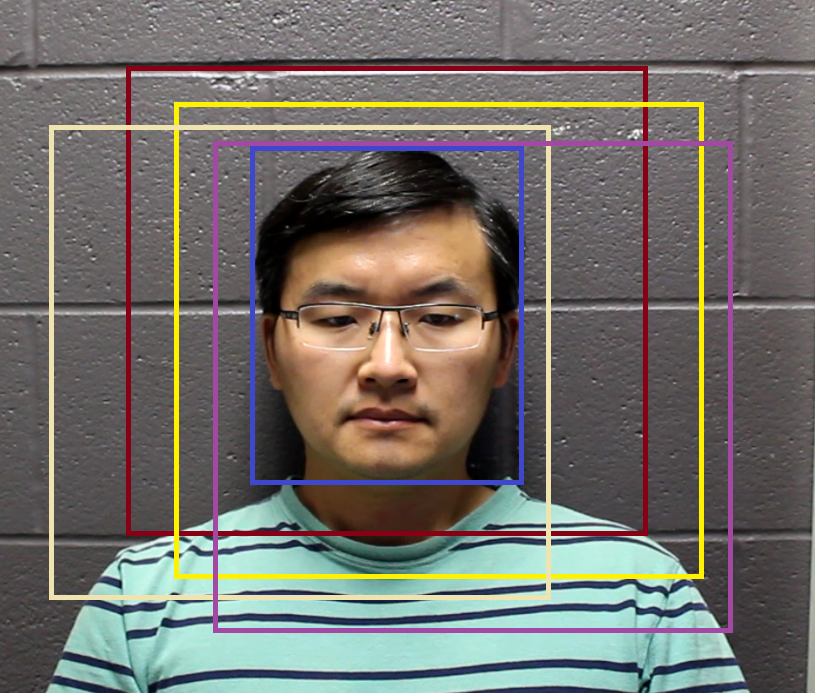
\includegraphics[width=0.7\linewidth]{aug}}
	\caption{نحوه برش زدن تصادفی چهره با مقداری از پس‌زمینه}
	\label{fig:aug}
\end{figure}

برای پیاده سازی کلاس بارگذاری داده یک
 \lr{Data loader} 
سفارشی نوشته شده است و همچنین برای آنکه استراتژی ترتیب تصادفی انتخاب ویدیو و استفاده مجدد از فریم‌های ویدیو متوالی پیاده شود یک تابع \lr{Batch sampler} سفارشی نوشته شده است. در پیاده‌سازی این تابع از مفهوم \lr{Iteration} در زبان برنامه‌نویسی پایتون استفاده شده است.
\section{معیارهای ارزیابی}
مسئله کشف تقلب یک مسئله طبقه‌بندی دو کلاسه است که در هنگام آزمون، معمولاً تعداد نمونه‌های واقعی و تقلبی یکسان نیستند. به همین دلیل معیار دقت شبکه یعنی تعداد نمونه‌های درست پیش‌بینی شده تقسیم بر تعداد کل نمونه‌ها ملاک خوبی برای قضاوت در مورد عملکرد شبکه نیست. 

بدین منظور از معیاری به نام نرخ خطای برابر 
\LTRfootnote{Equal Error Rate} ($EER$)
و ترسیم آن به ازای آستانه‌های مختلف، در قالب نمودار نرخ خطای برابر استفاده می‌شود. 
دو حالت برای تشکیل این نمودار مهم است. نرخ خطای قبول کردن
\LTRfootnote{False acceptance rate} ($FAR$)
 نمونه، که به معنی این است که برچسب واقعی چهره زنده بوده است اما به‌عنوان چهره تقلبی پیش‌بینی شده است. و نرخ خطای رد کردن
 \LTRfootnote{False rejection rate} ($FRR$)
  که به معنی این است که نمونه برچسب تقلبی دارد ولی به‌عنوان چهره زنده پیش‌بینی شده است.
\begin{equation} \label{eq:far}
	FAR = \frac{number\; of\; false\; accepted\; samples}{total\; number\; of\; fake\; samples}
\end{equation}
\begin{equation} \label{eq:frr}
	FAR = \frac{number\; of\; false\; rejected\; samples}{total\; number\; of\; real\; samples}
\end{equation}

معمولاً این مقدار بر اساس یک آستانه که یک پارامتر است محاسبه می‌گردد. برای مثال در شبکه‌ی عصبی مقدار تک نورون لایه آخر با تابع فعالسازی سیگموید، مقداری بین صفر و یک خواهد داشت. و با انتخاب یک سطح آستانه و مقایسه مقدار نورون لایه‌ی آخر با این سطح آستانه تصمیم‌گیری در مورد پیش‌بینی برچسب نمونه انجام می‌شود. نرخ خطای برابر، برابر با مقداری است که $FAR$ با $FRR$ برابر شود.

\begin{equation}\label{eq:taueer}
	\tau_{EER} = \argmin_{\tau}|FAR(\tau)-FRR(\tau)|
\end{equation}
\begin{equation}\label{eq:eer}
	EER=FAR(\tau_{EER})=FRR(\tau_{EER})
\end{equation}

در شکل
\ref{fig:eer}
این معیار را در قالب نمودار به ازای سطوح مختلف آستانه نشان می‌دهد. در دیتاست‌هایی که داده دارای سه قسمت آموزش، توسعه و آزمون است، معمولاً روی داده‌های آموزش وزن‌های شبکه به‌دست می‌آید و روی قسمت توسعه، پارامتر  
$\tau_{EER}$
 به دست خواهد آمد. و روی قسمت آزمون معیار نصف کل نرخ خطا
\LTRfootnote{Half total error rates}
  به‌صورت رابطه
\ref{eq:hter}
تعریف می‌شود.

\begin{equation}\label{eq:hter}
	HTER=\frac{FAR(\tau_{EER})+FRR(\tau_{EER})}{2}
\end{equation}

 \begin{figure}[ht]
	\centerline{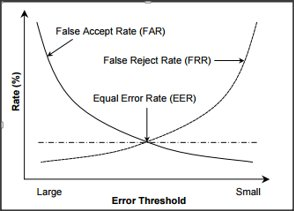
\includegraphics[width=0.5\linewidth]{eer}}
	\caption{نمودار میزان خطای برابر}
	\label{fig:eer}
\end{figure}

با تحلیل نمودار نرخ خطای برابر، می‌توان در مورد میزان عملکرد شبکه بحث کرد. هر چه که مقدار تقاطع منحنی $FRR$ و
$FAR$

پایین‌تر باشد، شبکه دقت بهتری دارد. همچنین مقدار
 $FRR$ و $FAR$
در نزدیکی‌های محل تقاطع نشان می‌دهد که شبکه چه میزان دو کلاس را از هم جدا کرده است. این یعنی نه تنها مقدار نرخ خطای برابر اهمیت دارد بلکه مطلوب این است که با تغییرات جزئی میزان سطح آستانه، نرخ خطا در اطراف آن نیز کم باشد. هر چه مقدار خطا در اطراف محل تقاطع دو منحنی کوچکتر باشد شبکه قابلیت تعمیم‌پذیری بیشتری روی داده‌های دیده نشده خواهد داشت.

یک معیار دیگر برای ارزیابی استفاده از استاندارد
 \lr{ISO/IEC 30107-3} 
است که در آن از نرخ خطای طبقه‌بندی ارائه حمله
\LTRfootnote{Attack Presentation Classification Error Rate}  ($APCER$) 
و نرخ خطای طبقه بندی ارائه خوب
\LTRfootnote{Bona Fide Presentation Classification Error Rate} ($BPCER$) 
تعریف می‌شود که در آن
$BPCER$
 معادل
$FRR$ 
است ولی
$APCE$
معادل بیشترین
$FAR$ 
به ازای ابزارهای حمله مختلف است.
منظور از ابزار حمله، حمله کاغذ چاپ‌شده یا حمله بازپخش است. رابطه 
\ref{eq:apcer}
نحوه محاسبه 
$APCER$
را نشان می‌دهد که در آن 
$PAI$
معادل ابزار حمله ارائه
\LTRfootnote{Presentation Attack Instrument}
است. در دیتاست‌های مورد استفاده در این پایان‌نامه 
$PAI$
پارامتر دو مقدار خواهد داشت که یکی برای حمله کاغذ چاپ‌شده و دیگری برای حمله بازپخش است.
همچنین متوسط نرخ خطای طبقه‌بندی 
\LTRfootnote{Average Classification Error Rate} $APCER$
به‌صورت میانگین 
$APCER$
 و 
$BPCER$ 
تعریف می‌شود.
\begin{equation}\label{eq:apcer}
	APCER=\max_{PAI=1,...,C}{FAR_{PAI}}
\end{equation}
\begin{equation}\label{eq:ACER}
	ACER=\frac{APCER+BPCER}{2}
\end{equation}
\section{عملکرد مدل در دیتاست‌ها}
این بخش به بررسی دقت روش پیشنهادی روی دیتاست‌های مختلف می‌پردازد. در ابتدا برای بررسی اثر بخشی روش پیشنهادی روی دیتاست \lr{Replay} که دیتاست نسبتاً کوچکی است، روش پیشنهادی بررسی می‌شود. این کار با هدف اثبات مفهوم
\LTRfootnote{Proof of concept}
 انجام می‌شود. و سپس روی دیتاست‌های دیگر دقت گزارش می‌شود.
\subsection{اثر عملگر \lr{LBP} قابل آموزش در دیتاست \lr{Replay}}
به‌منظور مقایسه‌ی روش‌های پیشنهادی و تأثیر آنها در بهبود دقت ابتدا یک شبکه \lr{ALEXNET} بدون عملگر \lr{LBP} با تابع هزینه \lr{BCE} به کار برده می‌شود. نمودار نرخ خطای برابر، برای این مورد به‌صورت شکل 
\ref{fig:eer-alex-bce} 
است. 
\begin{figure}[h]
	\centerline{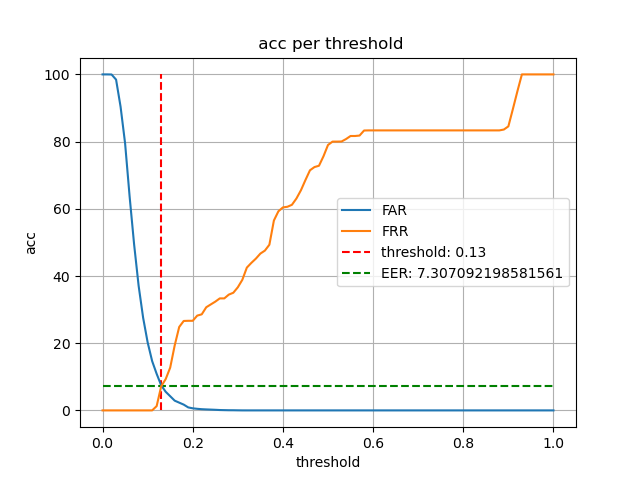
\includegraphics[width=0.65\linewidth]{eer-alex-bce}}
	\caption{نمودار خطای برابر برای شبکه \lr{ALEXNET} و تابع هزینه \lr{BCE}}
	\label{fig:eer-alex-bce}
\end{figure}

همانطور که مشاهده می‌شود با سطح آستانه متناظر با محل تقاطع دو نمودار برابر  
$\tau_{EER} = 0.13$
برای نورون آخر است که در این سطح آستانه نرخ خطای برابر  
$EER = 7.3 \%$
 روی داده دیده نشده به دست می‌آید. اما لازم است توجه شود تنها مقدار خطا مهم نیست و عملکرد نمودار در سایر مقادیر سطح آستانه نیز مهم است و در سطح آستانه 
 $\tau = 0.6$
  مقدار خطا 
$FRR=80\%$  
   است که بسیار زیاد است. هر چند که در این ناحیه خطا
  $FAR =0$
است. این تفاوت بین دو مقدار خطا نشان می‌دهد که دو کلاس  از یک دیگر جدا نشده اند و استخراج ویژگی به درستی صورت نگرفته است. همچنین در اطراف سطح آستانه 
  $\tau_{EER} = 0.13$
  با کمی تغییر در سطح آستانه مقدار خطا بزرگ می‌شود.


با استفاده از عملگر \lr{LBP} قابل آموزش پیش از \lr{ALEXNET} و تابع هزینه نیز کماکان \lr{BCE} باشد نمودار شکل
\ref{fig:eer-lbp}
به‌دست می‌آید.
\begin{figure}[h]
	\centerline{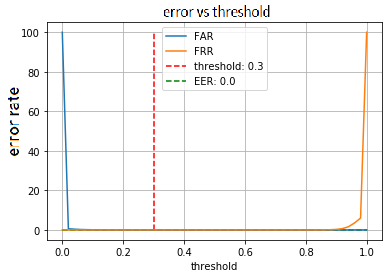
\includegraphics[width=0.65\linewidth]{eer-lbp}}
	\caption{نمودار خطای برابر هنگام استفاده از عملگر \lr{LBP} پیشنهادی}
	\label{fig:eer-lbp}
\end{figure}
همانطور که مشاهده می‌شود استفاده از تنها یک لایه 
\lr{LBP}
 پیش از \lr{ALEXNET} مقدار خطا را به صفر درصد رسانده است. همچنین وضعیت خطا در اطراف آستانه نیز بهبود یافته است.
از آنجا که افزودن یک لایه عملگر \lr{LBP} قابل آموزش، بار محاسباتی به شبکه اضافه می‌کند برای مقایسه دیگر نمودار آموزش شبکه با تابع هزینه \lr{BCE} و شبکه
 \lr{EfficientNet B0} 
با شروع از وزن‌های تصادفی، به صورت شکل 
\ref{fig:eer-eff}
است.
\begin{figure}[h]
	\centerline{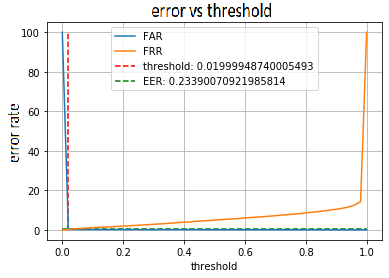
\includegraphics[width=0.65\linewidth]{eer-eff}}
	\caption{نمودار خطای برابر هنگام استفاده از شبکه \lr{EfficientNet B0}}
	\label{fig:eer-eff}
\end{figure}

این نمودار نشان می‌دهد لزوماً استفاده از شبکه پیچیده نمی‌تواند به نتیجه مطلوب برساند. 
لازم است توجه شود این نمودار بدین معنی نیست که لایه \lr{LBP} به همراه \lr{ALEXNET} قدرت بیشتری نسبت به شبکه \lr{Efficient net} دارد. بلکه در این کاربرد خاص و دیتاست \lr{Replay} که حجم داده کمی دارد استفاده از شبکه ساده‌تر اما هوشمندانه با توجه به مسئله، دقت بهتری را ایجاد می‌کند.
\subsection{اثر تابع هزینه \lr{ARCB} در دیتاست \lr{Replay}}
اکنون تنها از شبکه \lr{ALEXNET} بدون عملگر \lr{LBP} استفاده می‌شود ولی تابع هزینه \lr{ARCB} معرفی شده به‌جای تابع \lr{BCE} استفاده می‌شود. نمودار شکل
\ref{fig:eer-arcb}
نشان می‌دهد تغییر تابع هزینه بدون تغییری در ساختار می‌تواند تاثیرگذار باشد. نمودار در مقایسه با نمودارهای قبلی متقارن‌تر شده است .در این شکل میزان خطا در اطراف سطح آستانه صفر است ولی با دور شدن از سطح آستانه و نزدیک شدن به مقدار 0 و 1 خطا بیشتر می‌شود. این تأثیر حاشیه در تابع هزینه \lr{ARCB} است که موجب شده است دو کلاس با یک حاشیه از یک دیگر جدا شوند. در این حالت اگر مقدار آستانه در اطراف 
$\tau_{EER} = 0.67$
و در بازه 
$ 0.39\le \tau \le 0.75$
قرار داشته باشد مقدار خطا
 $FRR$ و $FAR$
 هر دو صفر خواهد بود. این باند اطمینان حاصل افزودن 
 $m$
در رابطه تابع هزینه
\lr{ARCB}
است که موجب جداسازی دو کلاس شده است. همچنین این تابع هزینه در مقایسه با تابع هزینه
\lr{BCE}
میزان خطای برابر را نیز کاهش داده است که بدین معناست که تابع هزینه، شبکه استخراج ویژگی را مجبور کرده است که به دنبال ویژگی‌های اساسی برای جداسازی دو کلاس با حاشیه باشد.
\begin{figure}[h]
	\centerline{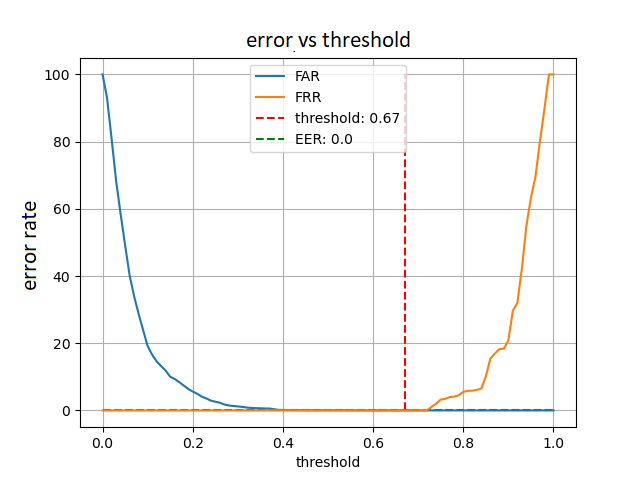
\includegraphics[width=0.65\linewidth]{eer-arcb}}
	\caption{نمودار خطای برابر هنگام استفاده از تابع هزینه \lr{ARCB} پیشنهادی}
	\label{fig:eer-arcb}
\end{figure}

\subsection{اثر تابع هزینه بر پایه شناسه‌ی اشخاص در دیتاست \lr{Replay}}
اکنون از ساختار ساده \lr{ALEXNET} استفاده می‌شود و تابع هزینه برای طبقه‌بند تابع \lr{BCE} است ولی تابع هزینه مبتنی بر شناسه اشخاص نیز به آن افزوده شده‌است. نمودار این حالت به‌صورت شکل 
\ref{fig:eer-pid}
است. همانطور که مشاهده می‌شود خطا در آستانه‌های 
$ 0.01\le \tau \le 0.8$
به‌صورت مطلق صفر است. این خطای صفر در این باند آستانه، نشان دهنده تاثیر تابع هزینه مبتنی بر شناسه اشخاص است. با به کار بردن این تابع هزینه و بدون هیچ تغییری در ساختار شبکه، وزن‌های شبکه به گونه‌ای تغییر یافته‌اند که ویژگی‌های اساسی مربوط به تقلب را پیدا کنند و به ویژگی‌های ظاهری چهره افراد توجه نکنند. 
\begin{equation}\label{eq:pid2}
	L_{PiD} = \sum_{l_1 \ne l_2,k_1 \ne k_2}{\frac{1}{N_i}d( X_{k_1}^{l},X_{k_2}^{l})+\frac{1}{N_j}\max(0,M-d( X_{k}^{l_1},X_{k}^{l_2} ))}
\end{equation}
چنان که در رابطه 
\ref{eq:pid2}
مشاهده می‌شود  عبارت اول این تابع هزینه باعث می‌شود جفت نمونه‌های دارای یک برچسب و شناسه شخص متفاوت به یک‌دیگر نزدیک‌تر شوند و در عبارت دوم جفت نمونه‌های یک شخص و متعلق به کلاس‌های متفاوت از یک‌دیگر به مقدار ‌
$M$
در فضای نرمالایز شده دور شوند.
\begin{figure}[!h]
	\centerline{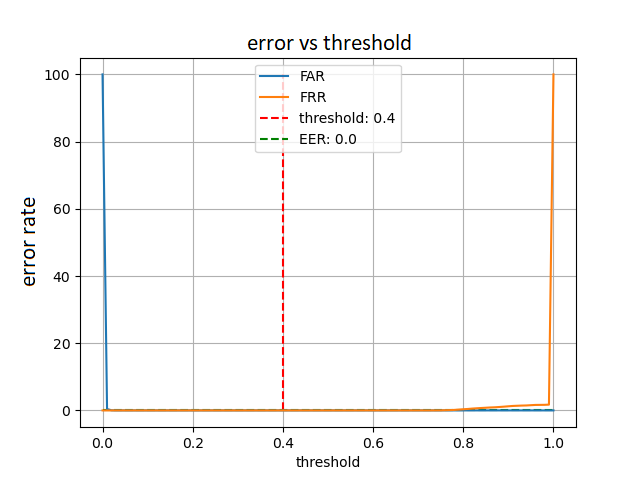
\includegraphics[width=0.65\linewidth]{eer-pid}}
	\caption{نمودار خطای برابر با استفاده از تابع هزینه مبتنی بر شناسه اشخاص}
	\label{fig:eer-pid}
\end{figure}

تا این قسمت اثر هر کدام از روش‌های پیشنهادی به تنهایی بررسی شده‌اند. برای ادامه فصل تمامی روش‌ها در کنار یک‌دیگر استفاده می‌شود. و شبکه استخراج ویژگی
\lr{EfficientNet B0} 
است. همچنین به‌منظور تسریع در همگرا شدن شبکه، قسمت استخراج ویژگی از وزن‌های آموزش دیده روی دیتاست
 \lr{ImageNet} \cite{deng2009imagenet}
استفاده می‌شود ولی این وزن‌ها حین آموزش تغییر می‌کند.


\subsection{نتایج روی دیتاست‌های \lr{CASIA} و \lr{MSU}}
دیتاست‌های \lr{MSU} و \lr{CASIA} نسبت به دیتاست \lr{Replay} دارای رزولوشن تصویر بیشتری هستند. این دیتاست‌ها بر خلاف دیتاست \lr{replay} که دارای سه قسمت آموزش، توسعه و آزمون است تنها دارای دو قسمت آموزش و آزمون می‌باشد. در جدول
\ref{tab:eercasiamsu}
 مقدار نرخ خطای برابر در قسمت آزمون دیتاست گزارش شده است.
\begin{table}[!h]
	\caption{خطای برابر روی دیتاست‌های \lr{CASI‌A} و ‌\lr{MSU}}
	\label{tab:eercasiamsu}
	\centering
	\onehalfspacing
	\begin{tabular}{|c|c|}
		\hline \lr{Dataset} &\lr{ EER (\%)}   \\
		\hline \lr{CASIA}   & \lr{0.54}     \\
		\hline \lr{MSU}     & \lr{0.0} \\
		   \hline
	\end{tabular} 
\end{table}

از آنجا که این دو دیتاست کمی قدیمی هستند رسیدن به نرخ خطای صفر چندان دشوار نیست. در پژوهش‌های اخیر در این حوزه، عمده گزارش‌های دقت روی دیتاست‌های \lr{SIW} و \lr{OULU} است. این دو دیتاست نسبت به دیتاست‌های قبلی جدیدتر و دارای حجم بیشتری هستند. به همین دلیل در پژوهش‌های اخیر بیشتر از این دو دیتاست استفاده شده است. هر کدام از این دو دیتاست دارای پروتکل‌های مختلفی هستند که حالت‌های مختلف برای بررسی تعمیم‌پذیری مدل را نشان می‌دهد.
\subsection{دقت در دیتاست \lr{SIW}}
در پروتکل اول دیتاست \lr{SIW} به بررسی تغییر حالت چهره می‌پردازد. بدین منظور برای آموزش از 60 فریم اول هر ویدیو استفاده می‌شود ولی برای آزمون از تمامی فریم‌های ویدیوهای تست استفاده می‌شود. از آنجا که در فریم­‌های ابتدایی هر ویدیو، کاربر صورت خود را تکان نمی‌دهد پس داده‌های آموزش تنها شامل تصاویر صورت با موقعیت ثابت در مقابل دوربین است. ولی داده‌های تست شامل همه حالت‌های حرکت چهره در ویدئو است. این پروتکل قابلیت تعمیم‌پذیری مدل ارائه شده را در حالت‌های مختلف چهره نشان می‌دهد. نتایج این حالت در جدول
\ref{tab:siw1}
همراه با مقایسه با برخی روش‌های معروف ذکر شده است.
\begin{table}[h]
	\caption{نرخ در پروتکل اول دیتاست \lr{SIW}}
	\label{tab:siw1}
	\centering
	\onehalfspacing
	\begin{tabular}{|c|c|c|l|}
	\hline \lr{ACER} & \lr{BPCER} & \lr{APCER} & \lr{Method}                \\
	\hline \lr{3.58} & \lr{3.58}  & \lr{3.58}  & \cite{liu2018learning} \lr{Auxiliary}    \\
	\hline \lr{0.25} & \lr{0.50}  & \lr{0}     & \cite{feng2020learning} \lr{LGSC}         \\
	\hline \lr{1}    & -     & -     & \cite{yang2019face} \lr{STASN}       \\
	\hline \lr{0.12} & \lr{0.17}  & \lr{0.07}  & \cite{yu2020searching} \lr{CDCN}             \\
	\hline \lr{0.4}  & \lr{0.17}  & \lr{0.64}  & \cite{wang2020deep} \lr{SGTD}      \\
	\hline \lr{0.4}  & \lr{0.17}  & \lr{0.69}  & \cite{li20203dpc}   \lr{3DPC-NET}   \\
	\hline \lr{0.13} & \lr{0.12}  & \lr{0.14}  & \lr{ARCB+PID}    \\ 
	 \hline         
	\end{tabular}
\end{table}

در پروتکل دوم از چهار نوع حمله‌ی بازپخش، هر بار یک حمله برای تست کنار گذاشته می‌شود و آموزش شبکه روی سه حمله‌ی بازپخش دیگر انجام می‌شود. پس برای این پروتکل چهار حالت مختلف وجود دارد که میانگین و واریانس دقت روی چهار حالت گزارش می‌شود. این پروتکل با هدف بررسی عمکرد روش پیشنهادی روی نوع حمله بازپخش دیده نشده طراحی شده است. نتایج در جدول 
\ref{tab:siw1}
گزارش شده است.
\begin{table}[!h]
	\caption{نرخ در پروتکل دوم دیتاست \lr{SIW}}
	\label{tab:siw2}
	\centering
	\onehalfspacing
	\begin{tabular}{|c|c|c|l|}
		\hline \lr{ACER}          & \lr{BPCER}       & \lr{APCER}         & \lr{Method}                  \\
		\hline \lr{0.57 ±0.69}    & \lr{0.57 ±0.69}  & \lr{0.57 ±0.69}    & \cite{liu2018learning} \lr{Auxiliary}     \\
		\hline \lr{0±0}           & \lr{0±0}         & \lr{0±0}           & \cite{feng2020learning} \lr{LGSC}           \\
		\hline \lr{0.28±0.05}     & -           & -             & \cite{yang2019face} \lr{STASN}           \\
		\hline \lr{0.04±0.5}      & \lr{0±0.09}      & \lr{0±0}           & \cite{yu2020searching} \lr{CDCN}            \\
		\hline \lr{0.02±0.04}     & \lr{0.04±0.08}   & \lr{0.0±0.0}       & \cite{wang2020deep} \lr{SGTD}        \\
		\hline \lr{0.45±0.14}     & \lr{0.43±0.06}   & \lr{0.46±0.28}     & \cite{li20203dpc}   \lr{3DPC-NET}   \\
		\hline \lr{0.0087±0.0151} & \lr{0.01±0.0173} & \lr{0.0075±0.0129} & \lr{ARCB+PID}                \\
		\hline         
	\end{tabular}
\end{table}

\subsection{دقت در دیتاست \lr{OULU}}
دیتاست \lr{OULU} نیز دارای چهار پروتکل مختلف است که در این پایان‌نامه دقت روی پروتکل اول و دوم گزارش شده است. 
دیتاست \lr{OULU} در سه مکان مختلف تصویر برداری شده است. در پروتکل اول روی ویدیوهای مربوط به مکان اول و دوم آموزش صورت می‌گیرد و در ویدیوهای مکان سوم آزمون انجام می‌گیرد. این پروتکل با این هدف ارائه شده است که قابلیت روش پیشنهادی با تغییر مکان تصویربرداری ارزیابی شود. نتایج به دست آمده به همراه مقایسه با روش‌هایی که روی این دیتاست روش خود را ارزیابی کرده‌اند در جدول
\ref{tab:oulu1}
گزارش شده است.
\begin{table}[h]
	\caption{دقت در پروتکل اول  دیتاست \lr{OULU}}
	\label{tab:oulu1}
	\centering
	\onehalfspacing	\begin{tabular}{|c|c|c|l|}
		\hline               
		\lr{ACER} & \lr{BPCER}          & \lr{APCER} & \lr{Method}                  \\
		\hline \lr{5.7}  & \lr{8.9}            & \lr{2.5}     & \cite{tu2020learning}\lr{GFA}  \\
		\hline \lr{1.6}  & \lr{1.6}            & \lr{1.6}      & \cite{liu2018learning} \lr{Auxiliary}  \\
		\hline \lr{1.5}  & \lr{1.7}            & \lr{1.2}      & \cite{jourabloo2018face} \lr{FaceDs}    \\
		\hline \lr{0.4}  & \lr{0}              & \lr{0.8}      & \cite{feng2020learning} \lr{LGSC}       \\
		\hline \lr{1.9}  & \lr{2.5}            & \lr{1.2}     & \cite{yang2019face} \lr{STASN}       \\
		\hline \lr{0.2}  & \lr{0}              & \lr{0.4}      & \cite{yu2020searching} \lr{CDCN}       \\
		\hline \lr{1.0}  & \lr{0.0}            & \lr{2.0}      & \cite{wang2020deep} \lr{SGTD}       \\
		\hline \lr{0.42} & \lr{0}              & \lr{0.83}    & \cite{george2019deep} \lr{DeepPixBis}\\
		\hline \lr{1.1}  & \lr{1.3}            & \lr{0.8}      & \cite{liu2020disentangling}\lr{STDN}     \\
		\hline \lr{1.2}  & \lr{0}              & \lr{2.3}     & \cite{li20203dpc}   \lr{3DPC-NET}   \\
		\hline \lr{2.29} & \lr{2}              & \lr{2.58}    & \lr{ARCB+PID} \\              
		\hline         
	\end{tabular}
\end{table}

در پروتکل دوم از دو حمله کاغذ چاپ شده و دو حمله بازپخش موجود در دیتاست یک حمله چاپ و یک حمله بازپخش برای آموزش و حمله چاپ و بازپخش دیگر برای تست استفاده می‌شود. هدف این پروتکل ارزیابی ابزار حمله دیده نشده در آموزش است. نتایج مربوط به دقت مدل ارائه شده در این پروتکل در جدول
\ref{tab:oulu2}
آورده شده است.


\begin{table}[ht]
	\caption{دقت در پروتکل‌ دوم دیتاست \lr{OULU}}
	\label{tab:oulu2}
	\centering
	\onehalfspacing
	\begin{tabular}{|c|c|c|l|}
		\hline             
		\lr{ACER} & \lr{BPCER}          & \lr{APCER} & \lr{Method}                  \\
		\hline     \lr{1.9}  & \lr{1.3}            & \lr{2.5}   & \cite{tu2020learning}\lr{GFA}  \\
		\hline     \lr{2.7}  & \lr{2.7}            & \lr{2.7}   & \cite{liu2018learning} \lr{Auxiliary}  \\
		\hline    \lr{4.3}  & \lr{4.4}            & \lr{4.2}   & \cite{jourabloo2018face} \lr{FaceDs}    \\
		\hline   \lr{0.7}  & \lr{0.6}            & \lr{0.8}   & \cite{feng2020learning} \lr{LGSC}       \\
		\hline     \lr{2.2}  & \lr{0.3}            & \lr{4.2}   & \cite{yang2019face} \lr{STASN}       \\
		\hline    \lr{1.3}  & \lr{0.8}            & \lr{1.8}   & \cite{yu2020searching} \lr{CDCN}       \\
		\hline  \lr{1.9}  & \lr{1.3}            & \lr{2.5}   & \cite{wang2020deep} \lr{SGTD}       \\
		\hline \lr{6.0}  & \lr{0.6}            & \lr{11.4}  & \cite{george2019deep} \lr{DeepPixBis}\\
		\hline \lr{1.9}  & \lr{1.6}            & \lr{2.3}   & \cite{liu2020disentangling}\lr{STDN}     \\
		\hline  \lr{3.0}  & \lr{2.8}            & \lr{3.1}   & \cite{li20203dpc}   \lr{3DPC-NET}   \\
		\hline  \lr{0.97} & \lr{0.97}           & \lr{0.97}  & \lr{ARCB+PID} \\              
		\hline         
	\end{tabular}
\end{table}

\subsection{نتایج در آزمون بین دیتاست}
همانطور که در قسمت‌های قبلی مشاهده شده است با روش‌های جدید یادگیری عمیق، رسیدن به نرخ خطای نزدیک صفر، دور از انتظار نیست. اما نحوه عملکرد مدل ارائه شده روی داده‌های دیده نشده با توزیع متفاوت همچنان موضوع چالشی و مهم در تحقیقات دانشگاهی است. یک مدل ممکن است روی یک دیتاست با توزیع خاص به دقت بسیار بالایی برسد ولی هنگام استفاده از این مدل در دنیای واقعی، ضعیف عمل کند.

نتایج ارائه شده تا اینجا دقت مدل درون دیتاست بوده است. یکی دیگر از مسائل مهم در حوزه کشف تقلب، بررسی دقت در آزمون بین دو دیتاست مختلف است. بدین منظور مدل روی یک دیتاست آموزش داده می‌شود و روی دیتاست دیگر ارزیابی می‌شود. 
برای بررسی دقت مدل در تست بین دیتاست، شبکه روی دیتاست \lr{CASIA} آموزش داده شده است و روی دیتاست \lr{Replay} ارزیابی شده است. نتایج این حالت در جدول
\ref{tab:cross}
به همراه دقت پژوهش‌های دیگر گزارش شده است. 
\begin{table}[!h]
	\caption{نتایج روی آزمون بین دیتاست}
	\label{tab:cross}
	\centering
	\onehalfspacing
	\begin{tabular}{|c|l|}
		\hline \lr{HTER \%}& \lr{Method}                  \\
		\hline \lr{31.5} & \cite{yang2019face} \lr{STASN}      \\
		\hline \lr{17}   & \cite{wang2020deep} \lr{SGTD}      \\
		\hline \lr{27.6} & \cite{liu2018learning} \lr{Auxiliary}   \\
		\hline \lr{28.5} & \cite{jourabloo2018face} \lr{FaceDs}     \\
		\hline \lr{21.4} & \cite{tu2020learning}\lr{GFA}       \\
		\hline \lr{27.4} & \cite{feng2020learning} \lr{LGSC}      \\
		\hline \lr{23.4} & \cite{li20203dpc}   \lr{3DPC-NET} \\
		\hline \lr{21.25} & \lr{ARCB+PID} \\ 
		\hline
	\end{tabular}
\end{table}

با مقایسه نتایج دقت در آزمون بین دیتاست و درون دیتاست تفاوت قابل ملاحظه خطا، دیده می‌شود.





		% فصل چهارم: نتایج
% !TeX root=../main.tex
\chapter{نتیجه‌گیری و کارهای آینده}
%\thispagestyle{empty} 
\section{نتیجه‌گیری}
در این پایان‌نامه به بررسی روش‌های موجود در حوزه امنیت سیستم‌های احراز هویت با استفاده از چهره پرداخته شد. روش‌های موجود به‌صورت عمده از سیگنال‌های کمکی نظیر عمق استفاده کرده‌اند. همچنین در بسیاری از روش‌ها از فریم‌های متوالی ویدئو برای استنتاج در مورد زنده یا تقلبی بودن چهره استفاده شده است. در این پایان‌نامه روشی مبتنی بر استفاده از تنها یک فریم توسعه داده شده است. همچنین روش پیشنهادی نیازی به عمق به‌عنوان سیگنال کمکی ندارد. با این وجود روش پیشنهادی در پروتکل‌های اول و دوم در دو دیتاست بزرگ و جدید در این حوزه به دقت‌های رقابتی با روش‌های دیگر رسیده است.

از آنجا که قسمت اصلی پردازش در روش پیشنهادی بر پایه شبکه \lr{efficient net} است حجم محاسباتی روش پیشنهادی بهینه است. از نظر زمان پاسخ، به‌دلیل استفاده از یک فریم، سریع است.
در این پایان‌نامه عملگری جدید بر پایه \lr{LBP} پیشنهاد شده است که خاصیت آموزش پذیری شبکه‌های \lr{CNN} را دارد. همچنین به‌علت توسعه تابع هزینه با حاشیه، قابلیت تفکیک‌پذیری شبکه بیشتر شده است. و استفاده از تابع هزینه مبتنی بر شناسه اشخاص موجب افزایش تعمیم‌پذیری شبکه شده است. مزیت استفاده از تابع هزینه در این است که افزایش دقت بدون افزودن بار محاسباتی به شبکه حاصل می‌شود. لذا در روش پیشنهادی با وجود آنکه زمان آموزش بیشتری نیاز دارد اما زمان تست شبکه تغییری نمی‌کند
\section{پیشنهاد کارهای آینده}
در این پژوهش از \lr{efficient net} استفاده شده است. پژوهش‌های بعدی می‌تواند شامل استفاده از ساختار از ابتدا طراحی شده باشد. همچنین به‌منظور افزایش دقت استفاده از ساختار توجه1 در شبکه می‌تواند مفید باشد. استفاده از دنباله ویدیویی به‌جای یک فریم برای افزایش دقت با یک ساختار جدید می‌تواند به افزایش دقت کمک کند. به‌منظور آنالیز بهتر بافت در تصویر، عملگر \lr{LBP} می‌تواند توسعه بیشتری داده شود به‌گونه‌ای که در تمامی لایه‌های شبکه به‌جای کانولوشن قرار بگیرد. همچنین تابع هزینه \lr{ARCB} می‌تواند مشابه روش
\cite{george2019deep}
روی یک صفحه مسطح به‌جای یک نورون نوشته شود. تابع هزینه مبتنی بر شناسه اشخاص می‌تواند به‌جای استفاده از شناسه اشخاص روی ویژگی‌های دیگر نظیر ابزار حمله باز نویسی شود. همچنین استفاده از عمق در کنار روش پیشنهادی ممکن است دقت بهتری به‌دست آورد.

در این پایان‌نامه تمرکز روی حملات چاپ و بازپخش بوده است. در این حوزه دیتاست‌هایی وجود دارند که شامل حملات استفاده از ماسک هستند. استفاده از روشی مشابه روش پیشنهادی روی دیتاست‌هایی که دارای تصاویر \lr{RGB} و \lr{IR} هستند نیز می‌تواند پژوهش بعدی باشد.

علاوه بر این، در این پایان‌نامه به‌منظور افزایش سرعت همگرایی، از آدام و شبکه با وزن‌های آموزش دیده شده استفاده شده است. پژوهش بعدی می‌تواند شامل استفاده از بهینه سازی \lr{SGD} و شروع با وزن‌های تصادفی و آموزش روی تعداد ایپاک زیاد باشد که ممکن است نقطه بهینه بهتری را پیدا کند.
		% فصل پنجم: بحث و نتیجه‌گیری

% مراجع
% اگر از استیل‌های natbib استفاده می‌کنید باید دو خط را در فایل commands.tex تغییر دهید.
\pagestyle{empty}
{
\small
\onehalfspacing
% \bibliographystyle{plain-fa} % or plainnat-fa for author-date
\bibliographystyle{IEEEtran}
\bibliography{./tex/MyReferences}
}

\pagestyle{fancy}

% \appendix
% فصلهای پس از این قسمت به عنوان ضمیمه خواهند آمد.

% دستورات لازم برای تبدیل «فصل آ» به «پیوست آ» در فهرست مطالب
\addtocontents{toc}{
    \protect\renewcommand\protect\cftchappresnum{\appendixname~}%
    \protect\setlength{\cftchapnumwidth}{\mylenapp}}
    
% دستورات لازم برای شماره‌گذاری صفحات پیوست‌ها بشکل آ-۱ (فعلا با glossaries سازگار نیست)
% \let\Chapter\chapter
%\pretocmd{\chapter}{
%  \clearpage
%  \pagenumbering{arabic}
%  \renewcommand*{\thepage}{\rl{\thechapter-\arabic{page}}}}{}{}
%%%%%%%%%%%%%%%%%%%%%%%%%%%%%%%%%%%%%
        

% !TeX root=../main.tex

\chapter{آشنایی سریع با برخی دستورات لاتک}
\label{app:latexIntro}
%\thispagestyle{empty}
در این فصل ویژگی‌های مهم و پرکاربرد زی‌پرشین و لاتک معرفی می‌شود. برای راهنمایی بیشتر و به‌کاربردن ویژگی‌های پیشرفته‌تر به راهنمای زی‌پرشین و راهنمای لاتک مراجعه کنید. برای آگاهی از دستورات لاتک که این خروجی را تولید کرده‌اند فایل \lr{appendix1.tex} را ملاحظه فرمایید.
\footnote{بیشتر مطالب این بخش از مثال 
\lr{xepersian\_example.tex}
گرفته شده‌اند که توسط آقای امیرمسعود پورموسی آماده شده است.}

\section{بندها و زیرنویس‌ها}
هر جایی از نوشتهٔ خود، اگر می‌خواهید به سر سطر بروید و یک بند (پاراگراف) تازه را آغاز کنید، باید یک خط را خالی بگذارید%
\footnote{یعنی دوبار باید کلید \lr{Enter} را بزنید.}
 مانند این:

حالا که یک بند تازه آغاز شده است، یک زیرنویس انگلیسی%
\LTRfootnote{English Footnote!}
 هم می‌نویسیم!
\section{فرمول‌های ریاضی}
\label{formula}

اینجا هم یک فرمول می‌آوریم که شماره دارد:
\begin{equation}\label{eq:yek}
A=\frac{c}{d}+\frac{q^2}{\sin(\omega t)+\Omega_{12}}
\end{equation}
در لاتک می‌توان به کمک فرمان 
\lr{\textbackslash label\{\}}
به هر فرمول یک نام نسبت داد. در فرمول بالا نام \lr{eq:yek} را برایش گذاشته‌ایم (پروندهٔ \lr{tex} همراه با این مثال را ببینید). این نام ما را قادر می‌کند که بعداً بتوانیم با فرمان
\lr{\textbackslash ref\{eq:yek\}}
به آن فرمول با شماره ارجاع دهیم. یعنی بنویسیم فرمول \ref{eq:yek}. 
لاتک خودش شمارهٔ این فرمول‌ها را مدیریت می‌کند.\footnote{یعنی اگر بعداً فرمولی قبل از این فرمول بنویسیم، خودبه‌خود شمارهٔ این فرمول و شمارهٔ ارجاع‌ها به این فرمول یکی زیاد می‌شود. دیگر نگران شماره‌گذاری فرمول‌های خود نباشید!} این هم یک فرمول که شماره ندارد:
$$A=|\vec{a}\times \vec{b}| + \sum_{n=0}^\infty C_{ij}$$

این هم عبارتی ریاضی مانند 
$\sqrt{a^2+b^2}$
 که بین متن می‌آید.
\subsection{یک زیربخش}
\label{zirbakhsh}

این زیربخش \ref{zirbakhsh} است؛ یعنی یک بخش درون بخش \ref{formula} است.
\subsubsection{یک زیرزیربخش}
این هم یک زیرزیربخش است. در لاتک می‌توانید بخش‌های تودرتو در نوشته‌تان تعریف کنید تا ساختار منطقی نوشته را به خوبی نشان دهید. می‌توانید به این بخش‌ها هم با شماره ارجاع دهید، مثلاً بخش فرمول‌های ریاضی شماره‌اش \ref{formula} است.
\section{نوشته‌های فارسی و انگلیسی مخلوط}
نوشتن یک کلمهٔ انگلیسی بین متن فارسی بدیهی است، مانند Example در این جمله.\footnote{هرچند بهتر است باز هم آن کلمه را مانند \lr{Example} در این جمله بنویسید.}
نوشتن یک عبارت چندکلمه‌ای مانند
 \lr{More than one word} کمی پیچیده‌تر است.

اگر ناگهان تصمیم بگیرید که یک بند کاملاً انگلیسی را بنویسید، باید:
\begin{latin}
This is an English paragraph from left to right. You can write as much as you want in it.
\end{latin}
\section{افزودن تصویر به نوشته}
پروندهٔ تصویر دلخواه خود را در کنار پروندهٔ \lr{tex} قرار دهید. سپس به روش زیر تصویر را در نوشتهٔ خود بیاورید:
\begin{latin}
\begin{verbatim}
\includegraphics{YourImageFileName}
\end{verbatim}
\end{latin}
به تصویرها هم مانند فرمول‌ها و بخش‌ها می‌توان با شماره ارجاع داد. مثلاً تصویر \ref{fig:shir} یک شیر علاقه‌مند به لاتک را در حال دویدن نشان می‌دهد. برای جزئیات بیشتر دربارهٔ روش گذاشتن تصویرها در نوشته باید راهنماهای لاتک را بخوانید.
\begin{figure}[ht]
\centerline{
\includegraphics[width=5cm]{lion}}
\caption{در این تصویر یک شیر علاقه‌مند به لاتک را در حال دویدن می‌بینید.}
\label{fig:shir}
\end{figure}

به تصویرها هم مانند فرمول‌ها و بخش‌ها می‌توان با شماره ارجاع داد. مثلاً تصویر بالا شماره‌اش \ref{fig:shir} است. برای جزئیات بیشتر دربارهٔ روش گذاشتن تصویرها در نوشته باید راهنماهای لاتک را بخوانید.

\section{محیط‌های شمارش و نکات}
برای فهرست‌کردن چندمورد، اگر ترتیب برایمان مهم نباشد:
\begin{itemize}
\item مورد یکم
\item مورد دوم
\item مورد سوم
\end{itemize}
و اگر ترتیب برایمان مهم باشد:
\begin{enumerate}
\item مورد یکم
\item مورد دوم
\item مورد سوم
\end{enumerate}
می‌توان موردهای تودرتو داشت:
\begin{enumerate}
\item مورد ۱
\item مورد ۲
\begin{enumerate}
\item مورد ۱ از ۲
\item مورد ۲ از ۲
\item مورد ۳ از ۲
\end{enumerate}
\item مورد ۳
\end{enumerate}
شماره‌گذاری این موردها را هم لاتک انجام می‌دهد.

\section{تعریف و قضیه}
برای ذکر تعریف، قضیه و مثال مثالهای ذیل را ببینید.
\begin{definition}
مجموعه همه ارزیابی‌های  (پیوسته)  روی $(X,\tau)$، دامنه توانی احتمالی
\index{دامنه توانی احتمالی}
$ X $
نامیده می‌شود.
\end{definition}
\begin{theorem}[باناخ-آلااغلو]
\index{قضیه باناخ-آلااغلو}
اگر $ V $ یک همسایگی $ 0 $ در فضای برداری 
\index{فضای!برداری}
 توپولوژیکی $ X $ باشد و 
\begin{equation}\label{eq1}
K=\left\lbrace \Lambda \in X^{*}:|\Lambda x|\leqslant 1 ; \ \forall x\in V\right\rbrace,
\end{equation}
آنگاه $ K $،  ضعیف*-فشرده است که در آن، $ X^{*} $ دوگان
\index{فضای!دوگان}
 فضای برداری توپولوژیکی $ X $ است به ‌طوری که عناصر آن،  تابعی‌های 
خطی پیوسته
\index{تابعی خطی پیوسته}
 روی $X$ هستند.
\end{theorem}
تساوی \eqref{eq1} یکی از مهم‌ترین تساوی‌ها در آنالیز تابعی است که در ادامه، به وفور از آن استفاده می‌شود.
\begin{example}
برای هر فضای مرتب، گردایه 
$$U:=\left\lbrace U\in O: U=\uparrow U\right\rbrace $$
از مجموعه‌های بالایی باز، یک توپولوژی تعریف می‌کند که از توپولوژی اصلی، درشت‌تر  است.
\end{example}
حال تساوی 
\begin{equation}\label{eq2}
\sum_{n=1}^{+\infty} 3^{n}x+7x=\int_{1}^{n}8nx+\exp{(2nx)}
\end{equation}
را در نظر بگیرید. با مقایسه تساوی \eqref{eq2} با تساوی \eqref{eq1} می‌توان نتیجه گرفت که ...


\section{چگونگی نوشتن و ارجاع به مراجع}
\label{Sec:Ref}


در لاتک به راحتی می‌توان مراجع خود را نوشت و به آنها ارجاع داد. به عنوان مثال برای معرفی کتاب گنزالس \cite{Gonzalez02book} به عنوان یک مرجع می‌توان آنرا به صورت زیر معرفی نمود:

\singlespacing
\begin{LTR}
\begin{verbatim}
\bibitem{Gonzalez02book}
Gonzalez, R.C., and Woods, R.E. {\em Digital Image Processing}, 3rd ed..
Prentice-Hall, Inc., Upper Saddle River, NJ, USA, 2006.
\end{verbatim}
\end{LTR}
\doublespacing

در دستورات فوق \lr{Gonzalez02book}  برچسبی است که به این مرجع داده شده است و با استفاده از دستور 
\verb!\cite{Gonzalez02book}!
می‌توان به آن ارجاع داد؛ بدون این که شماره‌اش را در فهرست مراجع‌مان بدانیم.

اگر این اولین مرجع ما باشد در قسمت مراجع به صورت زیر خواهد آمد:\\
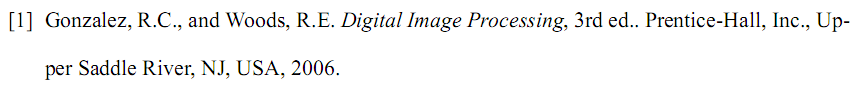
\includegraphics[width=\textwidth]{gonzalez.png}

این شیوهٔ تعریف مراجع بسیار ابتدایی است و اگر فرمت مراجع، ترتیب یا تعداد آنها را خواسته باشید تغییر دهید، به عنوان مثال ابتدا حرف اول نام نویسنده بیاید و سپس نام خانوادگی، باید همه کارها را به صورت دستی انجام دهید!
چون در یک \پ یا مقاله باید کنترل کاملی بر مراجع خود داشته باشید و به راحتی بتوانید قالب مراجع را عوض کنید، بنابراین می‌بایست از \lr{Bib\TeX} استفاده کنید که درپیوست  \ref{app:refMan} به  آن پرداخته خواهد شد.
		% پیوست اول: آشنایی مقدماتی با لاتک
% !TeX root=../main.tex

\chapter{‌جدول، نمودار و الگوریتم در لاتک}
\label{app:latex:more}
%\thispagestyle{empty}

در این بخش نمونه مثالهایی از جدول، شکل، نمودار، الگوریتم و معادلات ریاضی را در لاتک خواهیم دید.
دقت کنید که در پایان‌نامه‌ها و مقالات، باید قاعدهٔ «ارجاع به جلو%
\LTRfootnote{Forward Referencing}»
رعایت شود؛ یعنی ابتدا در متن به شمارهٔ شکل، جدول یا معادله اشاره شود و بعد از آن (زیر آن) خود شکل، جدول یا معادله رسم شود. (توضیحات بیشتر در قسمت
\ref{sec:floatObjs}).

\section{جدول}
دستور اصلی برای رسم جدول در لاتک 
\verb|tabular|
می‌باشد که جدول
\eqref{tab:motionModels}
با استفاده از آن کشیده شده است؛ در
\verb|tabular|
عرض جدول برابر با مجموع عرض ستون‌ها و حداکثر مساوی عرض متن است.
\begin{table}[ht]
\caption{مدلهای تبدیل.}
\label{tab:motionModels}
\centering
\onehalfspacing
\begin{tabular}{|r|c|l|r|}
	\hline نام مدل & درجه آزادی & تبدیل مختصات & توضیح \\ 
	\hline انتقالی & ۲ & $\begin{aligned} x'=x+t_x \\ y'=y+t_y \end{aligned}$  &  انتقال دوبعدی\\ 
	\hline اقلیدسی & ۳ & $\begin{aligned} x'=x\cos\theta - y\sin\theta+t_x \\ y'=x\sin\theta+y\cos\theta+t_y \end{aligned}$  &  انتقالی+دوران \\ 
	\hline 
\end{tabular} 
\end{table}

برای اینکه عرض جدول قابل کنترل باشد، باید از دستورات
\verb|tabularx|،
\verb|tabulary| یا
\verb|tabu|
استفاده کرد که راهنمای آنها در اینترنت وجود دارد.
مثلاً جدول
\ref{tab:motionModelsCont}
با
\verb|tabularx|
رسم شده که عرض جدول در آن ثابت بوده و ستون‌های از نوع
\verb|X|
عرض خالی جدول را پر می‌کنند.
\begin{table}[ht]
	\caption{مدلهای تبدیل دیگر.}
	\label{tab:motionModelsCont}
	\centering
	\onehalfspacing
	\begin{tabularx}{\textwidth}{|r|c|l|X|}
		\hline نام مدل & درجه آزادی & تبدیل مختصات & توضیح \\ 
		\hline مشابهت & ۴ & $\begin{aligned} x'=sx\cos\theta - sy\sin\theta+t_x \\ y'=sx\sin\theta+sy\cos\theta+t_y  \end{aligned}$  & اقلیدسی+تغییرمقیاس \\ 		
		\hline آفین & ۶ & $\begin{aligned} x'=a_{11}x+a_{12}y+t_x \\ y'=a_{21}x+a_{22}y+t_y \end{aligned}$  & مشابهت+اریب‌شدگی \\
		\hline
	\end{tabularx}
\end{table}

\section{معادلات ریاضی و ماتریس‌ها}
تقریباً هر آنچه دانشجویان برای نوشتن فرمول‌های ریاضی لازم دارند، در کتاب 
\lr{mathmode}
آمده است. کافیست در خط فرمان، دستور زیر را وارد کنید:
\begin{latin}
	\texttt{texdoc mathmode}
\end{latin}
متن زیر شامل انواعی از اشیاء ریاضی است که با ملاحظه کدش می‌توانید با دستورات آن آشنا شوید.\\
شناخته‌شده‌ترین روش تخمین ماتریس هوموگرافی الگوریتم تبدیل خطی مستقیم (\lr{DLT\LTRfootnote{Direct Linear Transform}}) است.  فرض کنید چهار زوج نقطهٔ متناظر در دو تصویر در دست هستند،  $\mathbf{x}_i\leftrightarrow\mathbf{x}'_i$   و تبدیل با رابطهٔ
  $\mathbf{x}'_i = H\mathbf{x}_i$
  نشان داده می‌شود که در آن:
\[\mathbf{x}'_i=(x'_i,y'_i,w'_i)^\top  \]
و
\[ H=\left[
\begin{array}{ccc}
h_1 & h_2 & h_3 \\ 
h_4 & h_5 & h_6 \\ 
h_7 & h_8 & h_9
\end{array} 
\right]\]
رابطه زیر را برای الگوریتم  \eqref{alg:DLT} لازم داریم.
\begin{equation}
\label{eq:DLT_Ah}
\left[
\begin{array}{ccc}
	0^\top & -w'_i\mathbf{x}_i^\top & y'_i\mathbf{x}_i^\top \\ 
	w'_i\mathbf{x}_i & 0^\top & -x'_i\mathbf{x}_i^\top \\ 
	- y'_i\mathbf{x}_i^\top & x'_i\mathbf{x}_i^\top & 0^\top
\end{array} 
\right]
\left(
\begin{array}{c}
	\mathbf{h}^1 \\ 
	\mathbf{h}^2 \\ 
	\mathbf{h}^3
\end{array} 
\right)=0
\end{equation}

\section{الگوریتم}

\subsection{الگوریتم ساده با دستورهای فارسی}
با مفروضات فوق، الگوریتم \lr{DLT} به صورت نشان داده شده در الگوریتم \eqref{alg:DLT}  خواهد بود.
\begin{algorithm}[ht]
\onehalfspacing
\caption{الگوریتم \lr{DLT} برای تخمین ماتریس هوموگرافی.} \label{alg:DLT}
\begin{algorithmic}[1]
\REQUIRE $n\geq4$ زوج نقطهٔ متناظر در دو تصویر 
${\mathbf{x}_i\leftrightarrow\mathbf{x}'_i}$،\\
\ENSURE ماتریس هوموگرافی $H$ به نحوی‌که: 
$\mathbf{x}'_i = H \mathbf{x}_i$.
  \STATE برای هر زوج نقطهٔ متناظر
$\mathbf{x}_i\leftrightarrow\mathbf{x}'_i$ 
ماتریس $\mathbf{A}_i$ را با استفاده از رابطهٔ \ref{eq:DLT_Ah} محاسبه کنید.
  \STATE ماتریس‌های ۹ ستونی  $\mathbf{A}_i$ را در قالب یک ماتریس $\mathbf{A}$ ۹ ستونی ترکیب کنید. 
  \STATE تجزیهٔ مقادیر منفرد \lr{(SVD)}  ماتریس $\mathbf{A}$ را بدست آورید. بردار واحد متناظر با کمترین مقدار منفرد جواب $\mathbf{h}$ خواهد بود.
  \STATE  ماتریس هوموگرافی $H$ با تغییر شکل $\mathbf{h}$ حاصل خواهد شد.
\end{algorithmic}
\end{algorithm}

\subsection{الگوریتم پیچیده و تودرتو با دستورهای فارسی}
الگوریتم \ref{alg:simulation-random}، یک الگوریتم ترکیبی و تودرتو است که با کمک دستورهای بستهٔ \lr{algorithmic} نوشته شده است.

\begin{algorithm}[p]
    \onehalfspacing
    \caption{الگوریتم اجرای برنامهٔ شبیه‌سازی}
    \label{alg:simulation-random}
    \begin{algorithmic}[1]
        \REQUIRE زمان $t_{max}$ به عنوان زمان لازم برای انجام شبیه سازی،\\
        \REQUIRE  گراف شبکه برای شبیه سازی،
        \ENSURE جدول تغییرات گراف از لحظهٔ ۰ تا t.
        \FOR {تمام لحظات در بازهٔ ۰ تا $t_{max}$}
            \FOR {تمام پیوند‌ها}
                \STATE محاسبهٔ ضریب و نرخ انتقال پیوند
                \STATE محاسبهٔ کیفیت و نرخ یادگیری
            \ENDFOR
            \FOR {تمام گره‌ها}
                \STATE محاسبهٔ نرخ انتقال گره
                \STATE محاسبهٔ وضعیت جدید
            \ENDFOR
            \IF {تغییرات از مقدار $\delta$ کمتر است}
                \STATE شکستن حلقه
                \COMMENT{این شرط برای پایان قبل از رسیدن به محدودیت زمانی است، اگر تغییرات کمتر از $\delta$ باشد}
            \ELSIF {زمان اجرای برنامه بیش از حد طول کشیده \AND $t>100$}
                \STATE شکستن حلقه
            \ENDIF
        \ENDFOR
        \PRINT {زمان اجرای برنامه}
        \RETURN {ماتریس تغییرات زمانی}
    \end{algorithmic}
\end{algorithm}

\subsection{الگوریتم با دستورهای لاتین}
الگوریتم \ref{alg:RANSAC} یک الگوریتم با دستورهای لاتین است.

\begin{algorithm}[ht]
\onehalfspacing
\caption{الگوریتم \lr{RANSAC} برای تخمین ماتریس هوموگرافی.} \label{alg:RANSAC}
\begin{latin}
\begin{algorithmic}[1]
\REQUIRE $n\geq4$ putative correspondences, number of estimations, $N$, distance threshold $T_{dist}$.\\
\ENSURE Set of inliers and Homography matrix $H$.
\FOR{$k = 1$ to $N$}
  \STATE Randomly choose 4 correspondence,
  \STATE Check whether these points are colinear, if so, redo the above step
  \STATE Compute the homography $H_{curr}$ by DLT algorithm from the 4 points pairs,
  \STATE $\ldots$ % الگوریتم کامل نیست
  \ENDFOR
  \STATE Refinement: re-estimate H from all the inliers using the DLT algorithm.
\end{algorithmic}
\end{latin}
\end{algorithm}

\section{کد}
درج کد به زبان‌های مختلف به سادگی امکان‌پذیر است. برنامه
\ref{code:matlabEx}
یک قطعه کد
\lr{MATLAB}
را نشان می‌دهد.
\begin{figure}[ht]
	\begin{LTR}
        \singlespacing
		\lstinputlisting[language=MATLAB, caption={نمونه کد \lr{MATLAB}}, label={code:matlabEx}]{MatlabExample.m}
        % \doublespacing
	\end{LTR}
\end{figure}

\section{تصویر}
نمونهٔ یک تصویر را در فصل قبل دیدیم. دو تصویر شیر کنار هم را نیز در شکل
\ref{fig:twoLion}
مشاهده می‌کنید.
\begin{figure}[ht]
\centering 
\subfloat[شیر ۱]{ \label{fig:twolion:one}

\includegraphics[width=0.3\textwidth]{lion}}
%\hspace{2mm}
\subfloat[شیر ۲]{ \label{fig:twolion:two}

\includegraphics[width=0.3\textwidth]{lion}}%
\caption{دو شیر}
\label{fig:twoLion} %% label for entire figure
\end{figure}

\section{نمودار}
لاتک بسته‌هایی با قابلیت‌های زیاد برای رسم انواع مختلف نمودارها دارد. مانند بسته‌های \lr{Tikz} و  \lr{PSTricks}. توضیح اینها فراتر از این پیوست کوچک است.%
\footnote{
مثال‌هایی از بکارگیری بسته
\lr{Tikz}
را می‌توانید در
\url{http://www.texample.net/tikz/examples/}
ببینید. توصیه می‌شود دانشجویانی که قصد درج اشکالی مانند گراف را در سند خود دارند، مثالهایی از سایت مذکور را ملاحظه فرمایند.
}
یک نمودار رسم شده با بستهٔ 
\lr{TikZ}
 در شکل 
\ref{fig:parabola}
نشان داده شده است.
\begin{figure}[t]
\centering
\begin{tikzpicture}[scale=2.5]
  \shade[top color=blue,bottom color=gray!50] 
      (0,0) parabola (1.5,2.25) |- (0,0);
  \draw (1.05cm,2pt) node[above] 
      {$\displaystyle\int_0^{3/2} \!\!x^2\mathrm{d}x$};

  \draw[style=help lines] (0,0) grid (3.9,3.9)
       [step=0.25cm]      (1,2) grid +(1,1);

  \draw[->] (-0.2,0) -- (4,0) node[right] {$x$};
  \draw[->] (0,-0.2) -- (0,4) node[above] {$f(x)$};

  \foreach \x/\xtext in {1/1, 1.5/1\frac{1}{2}, 2/2, 3/3}
    \draw[shift={(\x,0)}] (0pt,2pt) -- (0pt,-2pt) node[below] {$\xtext$};

  \foreach \y/\ytext in {1/1, 2/2, 2.25/2\frac{1}{4}, 3/3}
    \draw[shift={(0,\y)}] (2pt,0pt) -- (-2pt,0pt) node[left] {$\ytext$};

  \draw (-.5,.25) parabola bend (0,0) (2,4) node[below right] {$x^2$};
\end{tikzpicture}
\caption{یک نمودار زیبا با ارقام فارسی و قابلیت بزرگ‌نمایی بسیار، بدون از دست دادن کیفیت.}
\label{fig:parabola}
\end{figure}

\section{نحوه قرارگیری اشیای شناور}
\label{sec:floatObjs}
شکل‌ها، جداول و الگوریتم‌ها در لاتک اشیای شناور محسوب می‌شوند؛ یعنی خود لاتک تصمیم می‌گیرد آنها را در کجای صفحه ترسیم کند تا زیباتر باشد. اما می‌توان به لاتک توصیه کرد که آن را در قسمت خاصی از صفحه رسم کند. برای اینکه قاعدهٔ «ارجاع به جلو» رعایت شود باید فقط از پرچم
\verb|[ht]|
استفاده کرد، که می‌گوید اگر جا شد شکل را دقیقاً در همین مکان و در غیراینصورت در بالای صفحه بعد رسم کن.
بنابراین دستورات درج تصویر، جدول و الگوریتم به صورت زیر باید باشند:

\begin{latin}
\begin{verbatim}
	\begin{figure/table/algorithm}[ht]
		...
	\end{figure/table/algorithm}
\end{verbatim}
\end{latin}
		% پیوست دوم: جدول، نمودار و الگوریتم در لاتک
% !TeX root=../main.tex
\chapter{مراجع، واژه‌نامه و حاشیه‌نویسی}
\label{app:refMan}
%\thispagestyle{empty}

\section{مراجع و نقل‌قول‌ها}
\label{sec:refUsage}
منابعِ پایان‌نامه، پایه و اساس تحقیق شما به حساب می‌آیند و ضرورت انجام مطالعه و روش‌های به کار رفته در بسیاری از قسمت‌های آن، به کمک منابع صورت می‌گیرد. در استفاده از مراجع علمی در پایان‌نامه، باید سعی کنید بیشتر از
\textbf{منابع چاپ‌شده و مهم}
استفاده کنید و
\emph{ارجاع به داده‌های چاپ نشده، خلاصه‌ها و پایان‌نامه‌ها، سبب به‌هم‌خوردگی و کاهش اعتبار قسمت ارجاع منابع می‌شود.}
استفاده از منابع و نقل قول‌هایی به تحقیق شما ارزش می‌دهند که
\textbf{در راستای هدف تحقیق بوده و به آن اعتبار ببخشند.}
برخی از دانش‌جویان تصوّر می‌کنند که کثرت نقل‌قول‌ها و ارجاعات زیاد، مهم‌ترین معیار علمی شدن پایان‌نامه است؛ حال آنکه استناد به تعداد کثیری از منابع بدون مطالعه دقیق آنها و استفادهٔ مستقیم در پایان‌نامه، می‌تواند نشان‌دهندهٔ عدم احساس امنیت نویسنده باشد!

دو روش برای استفاده از نتایج، جملات، داده‌ها و روش‌های دیگران وجود دارد. یکی نقل‌قول مستقیم و دقیق است و دیگری استفاده غیرمستقیم در متن مقاله، که در ادامه به قواعد این دو نوع نقل‌قول و ارجاع‌دهی اشاره می‌کنیم:
\begin{description}
	\item[نقل‌قول مستقیم:]
	نقل‌قول مستقیم باید دقیق و بدون هیچ تغییری در جملات باشد. بهتر است این‌گونه نقل‌قول‌ها تا حد امکان کوتاه باشد. جملات کوتاه داخل گیومه قرار می‌گیرند و باید به منبع دقیق آن، طبق روش ارجاع‌دهی به منابع، اشاره شود. به عنوان مثال در
	\cite{persianbib87userguide}
	آمده است که:
	\begin{quote}
		«با استفاده از فیلد
		\lr{AUTHORFA}
		می‌توان معادل فارسی نام نویسندگان مقالات لاتین را در متن داشت. معمولاً در اسناد فارسی خواسته می‌شود که پس از ذکر معادل فارسی نام نویسنده، نام لاتین نویسنده(ها) به عنوان پاورقی درج شود
		\citep{persianbib87userguide}.»
	\end{quote}
	\item[نقل‌قول غیرمستقیم:]
	نقل‌قول غیرمستقیم به معنی استفاده از ایده‌ها، نتایج، روش‌ها و داده‌های دیگران در درون متنِ پایان‌نامه، ولی به سبک خودتان و متناسب و هماهنگ با روند پایان‌نامهٔ شماست. در این حالت نیز باید متناسب با شیوهٔ ارجاع‌دهی به آن استناد شود.
\end{description}

با توجه به وجود سبک‌های مختلف ارجاع‌دهی، باید
\textbf{روش قابل قبول و یکسانی}
در طول پایان‌نامه برای اشاره به مراجع در متن و همچنین تهیه فهرست مراجع در انتهای پایان‌نامه بکار رود. مثلاً برای پایان‌نامه‌های مهندسی می‌توان از سبک ارجاع‌دهی
\lr{IEEE}%
\LTRfootnote{\url{http://www.ieee.org/documents/ieeecitationref.pdf}}
یا
\lr{acm}
استفاده کرد. طبیعتاً باید تناظر یک‌به‌یک بین فهرست مراجع در انتهای گزارش و مراجع مورد استفاده در متن باشد%
\footnote{البته گاهی ممکن است محقق مرجعی را مورد مطالعه قرار داده لیکن در متن به آن اشاره نکرده باشد؛ برخی معتقدند در این موارد نیز آوردن آن در فهرست مراجع، اشکالی ندارد، به این شرط که از عنوان «فهرست منابع» به جای «فهرست مراجع» استفاده شود.}.

برای سهولت مدیریت مراجعِ \پ%
، اکیداً توصیه می‌شود از یک ابزار «مدیریت منابع» (با خروجی
\texorpdfstring{\lr{Bib\TeX}}{Bib\TeX}%
) همچون
\lr{Mendeley}،
\lr{Zotero},
\lr{EndNote}
یا
\lr{Citavi}
استفاده کنید.

\subsection{ مدیریت مراجع با  \texorpdfstring{\lr{Bib\TeX}}{Bib\TeX}}
در بخش \ref{Sec:Ref} اشاره شد که با دستور 
 \lr{\textbackslash bibitem}
  می‌توان یک مرجع را تعریف نمود و با فرمان
 \lr{\textbackslash cite}
  به آن ارجاع داد. این روش برای تعداد مراجع زیاد و تغییرات آنها مناسب نیست. برای مدیریت منابع زیاد، سه بستهٔ
\lr{BibTeX} (پیش‌فرض),
\lr{natbib}
(ارجاع‌دهی در متن به صورت نویسنده-سال)
و \lr{BibLaTeX} (جدید و منعطف‌پذیر)
وجود دارند. در ادامه توضیحاتی در مورد مدیریت منابع با \lr{BibTeX} و \lr{natbib} در زی‌پرشین خواهیم آورد که همراه با توزیع‌های معروف تِک عرضه می‌شوند
\footnote{روش \lr{BibLaTeX} هنوز برای متون فارسی به درستی ترجمه نشده است.}.

یکی از روش‌های قدرتمند و انعطاف‌پذیر برای نوشتن مراجعِ مقالات و مدیریت مراجع در لاتک، استفاده از  \lr{BibTeX} است.
 روش کار با بیب‌تک به این صورت است که مجموعهٔ همهٔ مراجعی را که در \پ استفاده کرده یا خواهیم کرد، 
در پروندهٔ جداگانه‌ای با پسوند
\lr{bib}
نوشته و به آن فایل در سند خودمان به صورت مناسب لینک می‌دهیم.
 کنفرانس‌ها یا مجله‌های گوناگون برای نوشتن مراجع، قالب‌ها یا قراردادهای متفاوتی دارند که به آنها استیل‌های مراجع گفته می‌شود.
 در این حالت به کمک ‌استیل‌های بیب‌تک خواهید توانست تنها با تغییر یک پارامتر در پروندهٔ ورودی خود، مراجع را مطابق قالب موردنظر تنظیم کنید. 
 بیشتر مجلات و کنفرانس‌های معتبر یک فایل سبک
 (\lr{BibTeX Style})
با پسوند \lr{bst} در وب‌گاه خود می‌گذارند که برای همین منظور طراحی شده است.

به جز نوشتن مقالات، این سبک‌ها کمک بسیار خوبی برای تهیهٔ مستندات علمی همچون پایان‌نامه‌هاست که فرد می‌تواند هر قسمت از کارش را که نوشت مراجع مربوطه را به بانک مراجع خود اضافه نماید. با داشتن چنین بانکی از مراجع، وی خواهد توانست به راحتی یک یا چند ارجاع به مراجع و یا یک یا چند بخش را حذف یا اضافه ‌نماید؛ 
مراجع به صورت خودکار مرتب شده و
\textbf{فقط مراجع ارجاع داده شده در قسمت کتاب‌نامه خواهندآمد.}
قالب مراجع به صورت یکدست مطابق سبک داده شده بوده و نیازی نیست که کاربر درگیر قالب‌دهی به مراجع باشد. 

\subsection{سبک‌های مورد تأیید دانشگاه تهران}
طبق «دستورالعمل نگارش و تدوین پایان‌نامه» دانشگاه تهران در
\cite{UTThesisGuide}،
ارجاع در متن می‌تواند مطابق با هر یک از دو الگوی هاروارد یا ونکوور باشد:
\singlespacing
\begin{description}
	\item[سیستم نویسنده-سال (هاروارد):]
	ذکر نام نویسنده و سال نشر در متن. در این الگو مراجع بر اساس حروف الفبا تنظیم می‌گردند.
	\item[سیستم شماره‌دار (ونکوور):]
	ارجاع به مراجع به کمک شماره در متن. در این الگو شماره هر مرجع به ترتیب ظاهر شدن آن در متن در داخل کروشه قرار می‌گیرد. فهرست مراجع نیز بر اساس شماره مرجع (نه حروف الفبا) تنظیم می‌گردد.
\end{description}
\doublespacing

در مدیریت منابع با
\lr{\textbf{BibTeX}}،
ارجاع‌ها در متن تنها به شکل
\textbf{شماره‌دار (ونکوور)}
امکان‌پذیر است، گرچه فهرست مراجع می‌تواند با روش‌های مختلف مرتب شود. اگر بخواهیم ارجاع‌ها در متن به صورت
\textbf{نویسنده-سال (هاروارد)}
باشد باید از بستهٔ
\lr{\textbf{natbib}}\LTRfootnote{Natural Sciences Citations \& References}
و استیل‌های مختلف آن استفاده کنیم.

هنگام استفاده از روش نویسنده-سال نوع پرانتزگذاری‌ها در وسط و انتهای جمله با هم فرق خواهد داشت. به مثال زیر مطابق با دستورالعمل
\cite{UTThesisGuide}
توجه کنید:

\textit{
ابتدا
\cite{Khalighi87xepersian}
بستهٔ زی‌پرشین را برای حروف‌چینی فارسی اختراع کرد. بعدها سبک‌های ارجاع‌دهی فارسی و قالب‌های پایان‌نامه نیز مبتنی بر آن ساخته شد
\citep{persianbib87userguide}.
ارجاع‌دهی به مراجع لاتین نیز در زی‌پرشین امکان‌پذیر است. مثلاً
\citelatin{Gonzalez02book}
یک کتاب انگلیسی است و به راحتی به مقالات انگلیسی نیز می‌توان ارجاع داد
\citeplatin{kim2016integrated}.}

در این مثال، ۴ ارجاع در وسط و انتهای جمله به مراجع فارسی و انگلیسی آمده است. وقتی از سیستم نویسنده-سال استفاده می‌کنید، بهتر است ارجاع‌های آخر جمله کلاً داخل پرانتر بیاید؛ بدین منظور باید به جای
\verb|\cite|
از
\verb|\citep|
استفاده کنید. اما در سیستم شماره‌دار چون تمام ارجاع‌ها داخل کروشه می‌آیند این امر اهمیت ندارد.\\
نمی‌توانید در متن فارسی، اسم لاتین محقق خارجی را بیاورید و برای جلوگیری از ایجاد ابهام، صرف‌نظر از نام لاتین هم مجاز نیست! توصیه می‌شود که نام محقق خارجی در متن با حروف فارسی و در پاورقی اسم تمام نویسندگان به صورت انگلیسی آورده شود. نحوهٔ رعایت این نکته را می‌توانید در کد مثال بالا ببینید.

گرچه در تمپلت ورد
\cite{UTThesisGuide}،
به صراحت ذکر شده که بهتر است برای پایان‌نامه‌های مهندسی از سبک 
\lr{IEEE}
استفاده شود (که از سیستم ونکوور تبعیت می‌کند)، اما ترتیب فهرست مراجع در
\lr{IEEE}
بر اساس ترتیب ارجاع در متن بوده و
\emph{مراجع انگلیسی و فارسی از هم تفکیک نمی‌شوند}
که متضاد با دستورالعمل
\cite{UTThesisGuide}
و نیز متضاد عرف اکثر پایان‌نامه‌های فارسی است.
بنابراین دقیقاً نمی‌توان سبک خاصی را برای مراجع پایان‌نامه‌های دانشگاه تهران اجبار کرد. مهم این است که
\textbf{سبک ارجاع‌دهی در تمام طول یک کتابچه}
(مثلاً پایان‌نامه، مقالات یک مجله یا کل یک کتاب) یکسان باشد. بهتر است
\textbf{بسته به حوزه پایان‌نامه}،
در این مورد با استاد راهنمای خود مشورت کنید.

\subsection{سبک‌های فارسی قابل استفاده در زی‌پرشین}
تعدادی از سبک‌های فارسی بسته
\lr{Persian-bib}%
\footnote{ برای اطلاع بیشتر به راهنمای بستهٔ
\lr{Persian-bib}
مراجعه فرمایید.}
که برای  زی‌پرشین آماده شده‌اند، عبارتند از:

\singlespacing
\begin{itemize}
\item \emph{سبک‌های شماره‌دار}:
	\begin{description}
	\item [unsrt-fa.bst] این سبک متناظر با \lr{unsrt.bst} می‌باشد. مراجع به ترتیب ارجاع در متن ظاهر می‌شوند.
	\item [plain-fa.bst] این سبک متناظر با \lr{plain.bst} می‌باشد. مراجع بر اساس نام‌خانوادگی نویسندگان، به ترتیب صعودی مرتب می‌شوند.
	 همچنین ابتدا مراجع فارسی و سپس مراجع انگلیسی خواهند آمد.
	\item [acm-fa.bst] این سبک متناظر با \lr{acm.bst} می‌باشد. شبیه \lr{plain-fa.bst} است.  قالب مراجع کمی متفاوت است. اسامی نویسندگان انگلیسی با حروف بزرگ انگلیسی نمایش داده می‌شوند. (مراجع مرتب می‌شوند)
	\item [ieeetr-fa.bst] این سبک متناظر با \lr{ieeetr.bst} می‌باشد. (مراجع مرتب نمی‌شوند)
	\end{description}
	
\item \emph{سبک‌های نویسنده-سال}:
	\begin{description}
	\item [plainnat-fa.bst] این سبک متناظر با \lr{plainnat.bst} می‌باشد. نیاز به بستهٔ \lr{natbib} دارد. (مراجع مرتب می‌شوند)
	\item [chicago-fa.bst] این سبک متناظر با \lr{chicago.bst} می‌باشد. نیاز به بستهٔ \lr{natbib} دارد. (مراجع مرتب می‌شوند)
	\item [asa-fa.bst] این سبک متناظر با \lr{asa.bst} می‌باشد. نیاز به بستهٔ \lr{natbib} دارد. (مراجع مرتب می‌شوند)
	\end{description}
\end{itemize}
\doublespacing

با استفاده از استیل‌های فوق می‌توانید به انواع مختلفی از مراجع فارسی و لاتین ارجاع دهید.
به عنوان مثال‌هایی از
\textbf{مراجع انگلیسی}،
مرجع
\cite{Baker02limits}\footnote{چون فیلد \lr{authorfa} برای این مرجع تعریف نشده در سبک نویسنده-سال با حروف لاتین به آن در متن ارجاع می‌شود که غلط است.}
مقالهٔ یک ژورنال، مرجع
\cite{Amintoosi09video}
مقالهٔ یک کنفرانس، مرجع
\citelatin{Gonzalez02book}
یک کتاب، مرجع
\cite{Khalighi07MscThesis}
پایان‌نامهٔ کارشناسی ارشد و مرجع
\citelatin{Borman04thesis}
یک رسالهٔ دکتری می‌باشد.\\
همچنین در میان
\textbf{مراجع فارسی},
مرجع
\cite{Vahedi87}
مقالهٔ یک مجله، مرجع
\cite{Amintoosi87afzayesh}
مقالهٔ یک کنفرانس، مرجع
\cite{Pedram80osool}
یک کتاب ترجمه‌شده با ذکر مترجمان و ویراستاران، مرجع
\cite{Pourmousa88mscThesis}
پایان‌نامهٔ کارشناسی ارشد%
\footnote{همان‌طور که در بخش
\ref{sec:refUsage}
اشاره شد، بهتر است زیاد از پایان‌نامه‌ها در مراجع استفاده نکنید.}،
مرجع
\cite{Omidali82phdThesis}
یک رسالهٔ دکتری و مراجع
\cite{persianbib87userguide, Khalighi87xepersian}
نمونه‌های متفرقه هستند.

\subsection{ساختار فایل مراجع}
برای استفاده از بیب‌تک باید مراجع خود را در یک فایل با پسوند \lr{bib} ذخیره نمایید. یک فایل \lr{bib} در واقع یک پایگاه داده از مراجع%
\LTRfootnote{Bibliography Database}
شماست که هر مرجع در آن به عنوان یک رکورد از این پایگاه داده
با قالبی خاص ذخیره می‌شود. به هر رکورد یک مدخل%
\LTRfootnote{Entry}
گفته می‌شود. یک نمونه مدخل برای معرفی کتاب \lr{Digital Image Processing} در ادامه آمده است:

\singlespacing
\begin{LTR}
\begin{verbatim}
@BOOK{Gonzalez02image,
  AUTHOR     = {Gonzalez,, Rafael C. and Woods,, Richard E.},
  TITLE      = {Digital Image Processing},
  PUBLISHER  = {Prentice-Hall, Inc.},
  YEAR       = {2006},
  ISBN       = {013168728X},
  EDITION    = {3rd},
  ADDRESS    = {Upper Saddle River, NJ, USA}
}
\end{verbatim}
\end{LTR}
\doublespacing

در مثال فوق، \lr{@BOOK} مشخصهٔ شروع یک مدخل مربوط به یک کتاب و \lr{Gonzalez02book} برچسبی است که به این مرجع منتسب شده است.
 این برچسب بایستی یکتا باشد. برای آنکه بتوان
\textbf{برچسب مراجع}
 را به راحتی به خاطر سپرد و حتی‌الامکان برچسب‌ها متفاوت با هم باشند، معمولاً از قوانین خاصی به این منظور استفاده می‌شود. یک قانون می‌تواند
\textbf{فامیل نویسنده اول + دورقم سال نشر + اولین کلمهٔ عنوان اثر}
باشد. به
\lr{AUTHOR}، \lr{TITLE}، $\dots$ و \lr{ADDRESS}
فیلدهای این مدخل گفته می‌شود، که هر یک با مقادیر مربوط به مرجع پر شده‌اند. ترتیب فیلدها مهم نیست. 

انواع متنوعی از مدخل‌ها برای اقسام مختلف مراجع همچون کتاب، مقالهٔ کنفرانس و مقالهٔ ژورنال وجود دارد که برخی فیلدهای آنها با هم متفاوت است. 
نام فیلدها بیانگر نوع اطلاعات آن می‌باشد. مثالهای ذکر شده در فایل \lr{MyReferences.bib} کمک خوبی برای شما خواهد بود. 
%این فایل یک فایل متنی بوده و با ویرایشگرهای معمول همچون \lr{Notepad++} قابل ویرایش می‌باشد. برنامه‌هایی همچون 
%\lr{TeXMaker}
% امکاناتی برای نوشتن این مدخل‌ها دارند و به صورت خودکار فیلدهای مربوطه را در فایل \lr{bib}  شما قرار می‌دهند.  
با استفاده از سبک‌های فارسی آماده شده، محتویات هر فیلد می‌تواند به فارسی نوشته شود؛ ترتیب مراجع و نحوهٔ چینش فیلدهای هر مرجع را سبک مورد استفاده  مشخص خواهد کرد.

\textbf{در فایل 
\lr{MyReferences.bib}
 که همراه با این \پ هست، مثال‌های مختلفی از مراجع آمده‌اند که برای درج مراجع خود، تنها کافیست مراجع‌تان را جایگزین موارد مندرج در آن نمایید.
}

برای بسیاری از مقالات لاتین حتی لازم نیست که مدخل مربوط به آنرا خودتان بنویسید. با جستجوی 
\textbf{نام مقاله + کلمه
\lr{bibtex}}
در اینترنت سایت‌های بسیاری همچون
\lr{ACM} و \lr{ScienceDirect}
را خواهید یافت که مدخل
\lr{bibtex}
مربوط به مقاله شما را دارند و کافیست آنرا به انتهای فایل
\lr{MyReferences.bib}
اضافه کنید.

\subsection{نحوه اجرای \texorpdfstring{\lr{Bib\TeX}}{Bib\TeX}}
پس از قرار دادن مراجع خود، برای ساخت فایل خروجی می‌توانید دستور زیر را (در ترمینال یا از طریق \lr{Texmaker}) اجرا کنید:%
\footnote{فایل \lr{latexmkrc} باید در کنار \lr{main.tex} وجود داشته باشد.}

\singlespacing
\begin{LTR}
	\begin{verbatim}
		latexmk -bibtex -pdf main.tex
	\end{verbatim}
\end{LTR}
\doublespacing
ابزار \lr{latexmk} مراحل مختلف ساخت خروجی لاتک را به طور خودکار و بهینه انجام می‌دهد و هر بار فقط مراحلی را که لازم باشد تکرار می‌کند.
روش دستی‌تر این است که یک بار \lr{XeLaTeX} را روی سند خود اجرا نمایید، سپس \lr{bibtex} و پس از آن هم ۲ بار \lr{XeLaTeX} را. در \lr{TeXMaker} کلید \lr{F11} و در \lr{TeXWorks} هم گزینهٔ \lr{BibTeX} از منوی \lr{Typeset}، \lr{BibTeX} را روی سند شما اجرا می‌کنند.

\section{واژه‌نامه‌ها و فهرست اختصارات}
\gls{Gloss}
یا فرهنگ لغات، مجموعه‌ای از اصطلاحات و تعاریف خاص و فنی است که معمولاً در انتهای یک کتاب می‌آید. چون پایان‌نامه خود یک متن تخصصی بلند محسوب می‌شود، استفاده از فرهنگ لغات در انتهای آن به شدت توصیه می‌شود، خصوصاً که احتمال استفاده از لغات تخصصی لاتین در آن بالاست.
واژه‌نامه‌هایی که در انتهای کتاب‌های انگلیسی می‌آیند معمولاً تک‌زبانه هستند و معنی یک اصطلاح تخصصی در آنها، عمدتاً به صورت یک
\gls{Description}
طولانی آورده می‌شود. اما چون در متون فارسی، آوردن لغات انگلیسی مجاز نیست و باید معادل فارسی آنها وارد شود، جهت رفع ابهام معمولاً واژه‌نامهٔ فارسی به انگلیسی (و برعکس) در انتهای کتاب درج شده و  
\glspl{Description}
در صورت نیاز در متن آورده می‌شوند.

فهرست
\glspl{Acronym}
شامل نمادهای کوتاهی است که اغلب از حروف ابتدایی کلمات یک عبارت طولانی ساخته شده‌اند. با اینکه
\glspl{Acronym}
با حروف (بزرگ) لاتین نوشته می‌شوند، اما چون کوتاهند استفاده از آنها در میان متن فارسی مجاز است. با این حال برای رفع ابهام، عرف است که فهرستی از آنها شامل معنی هر نماد، در کنار دیگر فهرست‌ها در ابتدای متن درج شود.

در این قالب پایان‌نامه، برای ساخت و مدیریت واژه‌نامه و فهرست اختصارات از بستهٔ پیشرفتهٔ
\lr{glossaries}
با موتور واژه‌نامه‌سازی
\lr{xindy}
استفاده می‌شود. تنظیمات بهینهٔ این بسته در فایل
\lr{glossaries-settings.tex}
عبارتند از:
\begin{itemize}
	\item
قبل از درج واژه‌ها در متن، باید مدخل آنها با دستور زیر (ترجیحاً در فایل جدای \lr{words.tex}) تعریف شود:
	\begin{LTR}
	\verb|\newword{Label}{Word}|\{واژه\}\{واژه‌ها\}
	\end{LTR}
	
	\item
قبل از وارد کردن علائم اختصاری در متن، باید مدخل آنها نیز (ترجیحاً در فایل \lr{acronyms.tex}) به صورت زیر تعریف شود:
	\begin{LTR}
	\verb|\newacronym{Label}{Acr}|\{معنی‌اختصار\}
	\end{LTR}

	\item
جهت درج یک علامت اختصاری یا معادل یک واژه تخصصی، کافی است از دستور
	\verb|gls{Label}|
در متن استفاده کنید. دستور
	\verb|glspl{Label}|
نیز برای آوردن معادل یک لغت در حالت جمع ساخته شده است.
	
	\item
هنگام اولین استفاده از یک معادل فارسی یا اختصار در متن، معادل انگلیسی یا معنی آن در پاورقی آورده می‌شود. در صورتی که هر یک از این پیش‌فرض‌ها را دوست ندارید با ویرایش فایل
	\lr{glossaries-settings.tex}
می‌توانید آن را تغییر دهید.

	\item
در انتهای پایان‌نامه با دستور
\verb|\printglossary|
فهرست کلمات استفاده‌شده به ترتیب الفبای فارسی (واژه‌نامه فارسی به انگلیسی) و الفبای انگلیسی (واژه‌نامه انگلیسی به فارسی) درج می‌شود.
\end{itemize}

به عنوان مثال، با مشاهدهٔ کد این نوشته، نحوهٔ درج معادل فارسی
\gls{RandomVariable}
را در متن مشاهده می‌کنید.
در نمایش واژهٔ
\gls{RandomVariable}
برای بار دوم، معادل لاتین در پاورقی نمی‌آید.
در مورد درج علائم اختصاری، مثلاً می‌توان به رابطهٔ
\gls{F}
اشاره کرد.

\section{حاشیه‌نویسی در نسخه پیش‌نویس}
اصلاح و بازبینی چندین و چندبارهٔ یک پایان‌نامه یا مقاله، از معمول‌ترین امور در نگارش آن می‌باشد. فرض کنید دانشجو پایان‌نامه یا مقالهٔ خود را (کامل یا ناقص) نوشته و می‌خواهد نظر استاد راهنما، اعضای آزمایشگاه یا دیگر متخصصین را در مورد آن جویا شود. به جز مشاورهٔ حضوری، تلفنی یا از طریق ایمیل، برای اظهارنظر دقیق بر نوشته، می‌توان از ابزارهای حاشیه‌نویسی در فایل
\lr{PDF}
یا \lr{tex}
نیز استفاده کرد.

یک راهکار مناسب برای حاشیه‌نویسی در فایل \lr{tex}، استفاده از بسته 
\lr{todonotes}
می‌باشد که آقای خلیقی به تازگی امکان استفاده از آن را برای فارسی‌زبانان نیز فراهم آورده‌اند.
بدین منظور، هر جایی که خواستید نکته یا نکاتی را در حاشیه متن یادداشت کنید، کافی است دستور زیر را وارد نمایید:
\begin{latin}
\verb|\todo{NOTE}|
\end{latin}
مثلاً استاد راهنما می‌تواند از دانشجو بخواهد که در بخشی توضیح بیشتری دهد.
\todo{
توضیح بیشتری لازم است.
}
استاد راهنما یا داور حتی می‌تواند محل پیشنهادی برای درج یک تصویر را نیز به راحتی برای دانشجو مشخص کند.
\missingfigure[figwidth=\textwidth,figcolor=white]{یک تصویر از خروجی الگوریتم 
\ref{alg:RANSAC}
را در اینجا قرار دهید.}
یکی دیگر از امکانات این بسته آن است که می‌توان فهرست نکات را در ابتدای سند داشت. بسته 
\lr{todonotes}
امکانات بسیاری دارد
\todo[fancyline,color=green!30]{مرجع این مطلب؟}
که در راهنمای آن معرفی شده است و با اجرای دستور زیر در خط فرمان می‌توانید آنها را مشاهده کنید:
\begin{latin}	
	\texttt{texdoc todonotes}
\end{latin}	
دقت کنید که توضیحات حاشیه‌ای و فهرست کارهای باقیمانده (نکات)،
\textbf{فقط در نسخه
\gls{Draft}}
قابل دیدن هستند و در نسخه نهایی، نمایش داده نخواهند شد.
برای استفاده از حالت
\gls{Draft}
باید گزینه 
\lr{draft}
به دستور 
\verb|\documentclass|
در ابتدای فایل 
\lr{main.tex}
اضافه شود.
هنگامی‌که سند شما در حالت 
\gls{Draft}
باشد:

\singlespacing
\begin{enumerate}
\item 
هیچ یک از صفحات آغازین پایان‌نامه، تا فهرست مطالب نمایش داده نمی‌شود (به جز صفحه اول).
\item
روی صفحه اول عبارت «پیش‌نویس» به صورت درشت و کم‌رنگ نمایش داده می‌شود.
\item
فهرست نکات درج شده توسط
\lr{todo}،
پس از فهرست اصلی و با عنوان «فهرست کارهای باقیمانده» نمایش داده می‌شود.
\item
شماره صفحاتی که به هر مرجع ارجاع داده شده است در بخش مراجع نمایش داده می‌شود
\footnote{اعمال گزینهٔ
\lr{pagebackref}
برای بستهٔ
\lr{hyperref}.
}.
\end{enumerate}
\doublespacing
هر یک از موارد بالا تا زمانی که نسخه نهایی \پ نیاز نباشد بسیار مورد توجه و مفید واقع می‌شوند.
   	% پیوست سوم: مراجع، واژه‌نامه و حاشیه‌نویسی

% برگرداندن شماره‌بندی صفحات فصول
% \let\chapter\Chapter
\pagenumbering{tartibi} % اول، دوم، ...
%\baselineskip=.75cm

% چاپ واژه‌نامه‌ها و نمایه 
\onehalfspacing
\cleardoublepage
\printglossary
\cleardoublepage
\printindex

\begin{latin}
\baselineskip=.6cm
\latinabstract
\latinTitlePage
\end{latin}
\label{LastPage}

\end{document}